\documentclass{beamer}
\usepackage[utf8]{inputenc}

\newcommand{\listingssize}{\normalsize}
%\newcommand{\titulek}{C++ - Dědičnost a polymorfizmus}
%\newcommand{\titulek}{C++ - Výjimky a jmenné prostory}
%\newcommand{\titulek}{C++ - Šablony}
%\newcommand{\titulek}{C++ - Přetěžování operátorů}
%\newcommand{\titulek}{C++ - STL}
%\newcommand{\titulek}{C++ - Datové proudy}
%\newcommand{\titulek}{C++ - Kontejnery}
%\newcommand{\titulek}{C++ - Iterátory}
\newcommand{\titulek}{C++ - Algoritmy}
\newcommand{\autor}{Ing. Roman Diviš}
\newcommand{\predmet}{\titulek}

\usepackage[czech]{babel} 
%\usepackage[IL2,T1,T2A]{fontenc} 
\usepackage[T1]{fontenc} 

%\usetheme{JuanLesPins}
\usetheme{Boadilla}

%%%%%%%%%%%%%%%%%%%%%%%%%%%%%%%%%%%%%%%%%%%%%%%%%%%
\setbeamertemplate{footline}[frame number]{}
\setbeamertemplate{navigation symbols}{}
%\setbeamertemplate{blocks}[rounded][shadow=false]
\setbeamertemplate{blocks}[default]
%\setbeamertemplate{background canvas}[vertical shading][bottom=white,top=structure.fg!5]


% pro vkládání obrázků
\usepackage{graphicx} 
% pro použití víceřádkových komentářů
\usepackage{verbatim} 
% H modifikátor figure
\usepackage{float}
% barvičky
\usepackage{xcolor,colortbl}
\usepackage{subfig}


\newcommand{\rc}{\cellcolor{red!25}}
\newcommand{\bc}{\cellcolor{blue!25}}
\newcommand{\gc}{\cellcolor{gray!25}}
\newcommand{\grc}{\cellcolor{green!25}}

\newcommand{\cpp}[1]{{\footnotesize$^{C++#1}$}}

\newcommand{\thisse}{\color{blue}\textbf{{\tiny this}}$\searrow$}
\newcommand{\thise}{\color{blue}\textbf{{\tiny this}}$\rightarrow$}

\usepackage{tikz}
\usetikzlibrary{arrows,shapes}
\newcommand{\tikzmark}[1]{\tikz[remember picture] \node[coordinate] (#1) {#1};}

% listingy
\usepackage{listings}

\newcommand{\commentcolor}{\color[rgb]{0.133,0.545,0.133}}
\lstset{
  tabsize=2,
  language=matlab,
  basicstyle=\listingssize,% \ttfamily,
  %upquote=true,
  mathescape=true,
  aboveskip=0pt, %{1.5\baselineskip},
  columns=fullflexible,
  showstringspaces=false,,
  breaklines=true,
  prebreak = \raisebox{0ex}[0ex][0ex]{\ensuremath{\hookleftarrow}},
  frame=none,
  showtabs=false,
  showspaces=false,
  showstringspaces=false,
  identifierstyle=\ttfamily,
  keywordstyle=\color[rgb]{0,0,1}\bfseries,
  commentstyle=\color[rgb]{0.133,0.545,0.133},
  stringstyle=\color[rgb]{0.627,0.126,0.941},
  language=Java,
  inputencoding=utf8,
  extendedchars=true,
%  literate={á}{{\'a}}1 {ã}{{\~a}}1 {é}{{\'e}}1
  literate={á}{{\'a}}1 {ã}{{\~a}}1 {é}{{\'e}}1 {ž}{{\v{z}}}1 {ý}{{\'y}}1 {ě}{{\v{e}}}1 {ř}{{\v{r}}}1 {í}{{\'i}}1 {ů}{{\r{u}}}1 {č}{{\v{c}}}1 {ú}{{\'u}}1 {š}{{\v{s}}}1 {ť}{{\v{t}}}1 {Č}{{\v{C}}}1 {Š}{{\v{S}}}1 {ň}{{\v{n}}}1 {Ř}{{\v{R}}}1 {ó}{{\'o}}1
}

	
\lstloadlanguages{[11]C++}
\lstset{language=[11]C++}
%\lstset{language=[Sharp]C}
\lstset{morekeywords={final,override}}
\lstset{escapeinside={<@}{@>}}

%\usepackage{pxfonts}
% odkazy v pdf
\usepackage{hyperref}

\author{\autor}
\title{\titulek}
\institute{UPCE/FEI/KST}
\date{}

\hypersetup{
pdftitle={\titulek},
pdfsubject={\predmet},
pdfauthor={\autor}
}









\mode<handout>
{
  \usepackage{pgf}
  \usepackage{pgfpages}

\pgfpagesdeclarelayout{4 on 1 boxed}
{
  \edef\pgfpageoptionheight{\the\paperheight} 
  \edef\pgfpageoptionwidth{\the\paperwidth}
  \edef\pgfpageoptionborder{0pt}
}
{
  \pgfpagesphysicalpageoptions
  {%
    logical pages=4,%
    physical height=\pgfpageoptionheight,%
    physical width=\pgfpageoptionwidth%
  }
  \pgfpageslogicalpageoptions{1}
  {%
    border code=\pgfsetlinewidth{2pt}\pgfstroke,%
    border shrink=\pgfpageoptionborder,%
    resized width=.5\pgfphysicalwidth,%
    resized height=.5\pgfphysicalheight,%
    center=\pgfpoint{.25\pgfphysicalwidth}{.75\pgfphysicalheight}%
  }%
  \pgfpageslogicalpageoptions{2}
  {%
    border code=\pgfsetlinewidth{2pt}\pgfstroke,%
    border shrink=\pgfpageoptionborder,%
    resized width=.5\pgfphysicalwidth,%
    resized height=.5\pgfphysicalheight,%
    center=\pgfpoint{.75\pgfphysicalwidth}{.75\pgfphysicalheight}%
  }%
  \pgfpageslogicalpageoptions{3}
  {%
    border code=\pgfsetlinewidth{2pt}\pgfstroke,%
    border shrink=\pgfpageoptionborder,%
    resized width=.5\pgfphysicalwidth,%
    resized height=.5\pgfphysicalheight,%
    center=\pgfpoint{.25\pgfphysicalwidth}{.25\pgfphysicalheight}%
  }%
  \pgfpageslogicalpageoptions{4}
  {%
    border code=\pgfsetlinewidth{2pt}\pgfstroke,%
    border shrink=\pgfpageoptionborder,%
    resized width=.5\pgfphysicalwidth,%
    resized height=.5\pgfphysicalheight,%
    center=\pgfpoint{.75\pgfphysicalwidth}{.25\pgfphysicalheight}%
  }%
}


\pgfpagesdeclarelayout{4 on 1 b}
{
  \edef\pgfpageoptionheight{\the\paperheight} 
  \edef\pgfpageoptionwidth{\the\paperwidth}
  \edef\pgfpageoptionborder{0pt}
}
{
  \pgfpagesphysicalpageoptions
  {%
    logical pages=4,%
    physical height=\pgfpageoptionheight,%
    physical width=\pgfpageoptionwidth%
  }
  \pgfpageslogicalpageoptions{1}
  {%
%    border code=\pgfsetlinewidth{2pt}\pgfstroke,%
%    border shrink=\pgfpageoptionborder,%
    resized width=.5\pgfphysicalwidth,%
    resized height=.5\pgfphysicalheight,%
    center=\pgfpoint{.25\pgfphysicalwidth}{.75\pgfphysicalheight}%
  }%
  \pgfpageslogicalpageoptions{2}
  {%
%   border code=\pgfsetlinewidth{2pt}\pgfstroke,%
%    border shrink=\pgfpageoptionborder,%
    resized width=.5\pgfphysicalwidth,%
    resized height=.5\pgfphysicalheight,%
    center=\pgfpoint{.75\pgfphysicalwidth}{.75\pgfphysicalheight}%
  }%
  \pgfpageslogicalpageoptions{3}
  {%
%    border code=\pgfsetlinewidth{2pt}\pgfstroke,%
%    border shrink=\pgfpageoptionborder,%
    resized width=.5\pgfphysicalwidth,%
    resized height=.5\pgfphysicalheight,%
    center=\pgfpoint{.25\pgfphysicalwidth}{.25\pgfphysicalheight}%
  }%
  \pgfpageslogicalpageoptions{4}
  {%
%    border code=\pgfsetlinewidth{2pt}\pgfstroke,%
%    border shrink=\pgfpageoptionborder,%
    resized width=.5\pgfphysicalwidth,%
    resized height=.5\pgfphysicalheight,%
    center=\pgfpoint{.75\pgfphysicalwidth}{.25\pgfphysicalheight}%
  }%
}


  \pgfpagesuselayout{4 on 1 b}[a4paper, border shrink=5mm, landscape]
  \nofiles
}





\newcommand{\hkapitola}[1]{
\section{#1}
\begin{frame}
\begin{block}{}
\Huge
\centering
#1
\end{block}
\end{frame}
}



\newcommand{\kapitola}[1]{
\subsection{#1}
\begin{frame}
\begin{block}{}
\Large
\centering
#1
\end{block}
\end{frame}
}


\newcommand{\pkapitola}[1]{
\subsubsection{#1}
\begin{frame}
\begin{block}{}
\large
\centering
#1
\end{block}
\end{frame}
}


\newcommand{\pulsirkycol}{.45\textwidth}
\newcommand{\tretinasirkycol}{.275\textwidth}

\newcommand{\raisesym}[1]{\raisebox{0.5\depth}{#1}}

\newcommand{\NO}{\scriptsize\raisesym{$\times$}}
\newcommand{\YES}{\scriptsize\raisesym{\checkmark}}
\newcommand{\WARNING}{\scriptsize\raisesym{\fontencoding{U}\fontfamily{futs}\selectfont\char 66\relax}}

\newcommand{\dcc}{\color[rgb]{0.35,0.35,0.35}}

\newcommand{\nezkouskove}{%\setbeamertemplate{background canvas}[vertical shading][bottom=violet!5,top=violet!5]
\setbeamertemplate{background canvas}{%
\begin{tikzpicture}
    \clip (0,0) rectangle (\paperwidth,\paperheight);
    \fill[color=violet] (0,\paperheight) rectangle (\paperwidth,\paperheight-5pt);
    \fill[color=violet] (0,0) rectangle (\paperwidth,5pt);

	\fill[color=white] (.90\paperwidth,0) rectangle (\paperwidth,10pt);
\end{tikzpicture}
}
}
%\newcommand{\zkouskove}{\setbeamertemplate{background canvas}[vertical shading][bottom=white,top=structure.fg!5]}
\newcommand{\zkouskove}{\setbeamertemplate{background canvas}[vertical shading][bottom=white,top=white]}

\newenvironment<>{deprecatedblock}[1]{
  \begin{actionenv}#2
    \def\insertblocktitle{#1}
    \par
    \mode<presentation>{
      \setbeamercolor{block title}{fg=white,bg=gray!90!white}
      \setbeamercolor{block body}{fg=black,bg=gray!30}
      \setbeamercolor{itemize item}{fg=gray!20!white}
      \setbeamertemplate{itemize item}[triangle]
    }
    \usebeamertemplate{block begin}}
    {\par\usebeamertemplate{block end}\end{actionenv}}

\newenvironment<>{noteblock}[1]{
  \begin{actionenv}#2
    \def\insertblocktitle{#1}
    \par
    \mode<presentation>{
      \setbeamercolor{block title}{fg=orange!60!black,bg=yellow!60!white}
      \setbeamercolor{block body}{fg=black,bg=yellow!10}
      \setbeamercolor{itemize item}{fg=gray!20!black}
      \setbeamertemplate{itemize item}[triangle]
    }
    \usebeamertemplate{block begin}}
    {\par\usebeamertemplate{block end}\end{actionenv}}

\newenvironment<>{bonusblock}[1]{
  \begin{actionenv}#2
    \def\insertblocktitle{#1}
    \par
    \mode<presentation>{
      \setbeamercolor{block title}{fg=yellow,bg=violet!80!black}
      \setbeamercolor{block body}{fg=black,bg=lime!10!white}
      \setbeamercolor{itemize item}{fg=gray!20!black}
      \setbeamertemplate{itemize item}[triangle]
    }
    \usebeamertemplate{block begin}}
    {\par\usebeamertemplate{block end}\end{actionenv}}



\newenvironment{yesblock}{\begin{exampleblock}{\YES}}{\end{exampleblock}}
\newenvironment{noblock}{\begin{alertblock}{\NO}}{\end{alertblock}}
\newenvironment{oldblock}{\begin{deprecatedblock}{\WARNING}}{\end{deprecatedblock}}

%[totalwidth=\textwidth]
\newenvironment{twocols}{\begin{columns}\begin{column}{\pulsirkycol}}{\end{column}\end{columns}}
\newcommand{\twocolssep}{\end{column}\begin{column}{\pulsirkycol}}

\newenvironment{threecols}{\begin{columns}\begin{column}{\tretinasirkycol}}{\end{column}\end{columns}}
\newcommand{\threecolssep}{\end{column}\begin{column}{\tretinasirkycol}}

\newenvironment{bitemize}{\begin{block}{}\begin{itemize}}{\end{itemize}\end{block}}


%%\setbeamercolor{background canvas}{bg=violet}


% Blocks:
% block
% exampleblock <- yesblock
% alertblock <- noblock
% noteblock
% deprecatedblock <- oldblock
% bonusblock
% twocols + cmd twocolssep
% threecols + cmd threecolssep
% bitemize - block + itemize
% Commands:
% \NO \YES \WARNING \pulsirkycol


%%%%%%%%%%%%%%%%%%%%%%%%%%%%%%%%%%%%%%%%%%%%%%%%%%%%%%%%%%%%%%%%%%%%%%%%
\begin{document}

%\section{\titulek}

\begin{frame}
  \titlepage
\end{frame}

\begin{frame}{Obsah}
  \tableofcontents%[currentsection]
\end{frame}
%\begin{frame}{Obsah}
  \tableofcontents[currentsection]
\end{frame}

% 01
%\hkapitola{Požadavky, zápočet, zkouška}


\begin{frame}[fragile]
\begin{block}{Přednáší, zkouší \& studenty děsí}
\begin{itemize}
\item Ing. Roman Diviš
\item roman.divis@upce.cz
\item konzultační hodiny - vizte upce.cz
\end{itemize}
\end{block}

\begin{block}{Cvičí}
\begin{itemize}
\item Ing. Jan Merta
\item jan.merta@student.upce.cz
\end{itemize}
\end{block}
\end{frame}



\begin{frame}[fragile]
\begin{block}{Zápočet}
\begin{itemize}
\item docházka
\item samostatně vypracovaná semestrální práce
\end{itemize}
\end{block}

\begin{block}{Zkouška}
\begin{itemize}
\item teoretický test (10 minut)
\item program dle zadání (cca 150 minut)
\end{itemize}
\end{block}
\end{frame}



\begin{frame}[fragile]
\vfill
\begin{figure}
\centering
\includegraphics[width=0.48\linewidth]{img/mindmap.pdf}
%\caption{}
%\label{fig:mindmap}
\end{figure}
\vfill
\end{frame}
%\hkapitola{Použitý styl v přednáškách}


\begin{frame}[fragile]
%\frametitle{Styly}
\begin{block}{Základní informace} 
Lorem ipsum dolor sit amet, consectetur adipiscing elit.
\end{block}

\begin{exampleblock}{Příklad}
Nullam mattis efficitur aliquam.
\end{exampleblock}

\begin{alertblock}{Chyba / příklad s chybou / nekorektní použití} 
Sed aliquam iaculis massa, vel tincidunt lacus tincidunt eget.
\end{alertblock}

\begin{noteblock}{Poznámka (teorie, vhodné k zapamatování)}
Proin porta urna ut ipsum ornare, a ultricies elit dictum.
\end{noteblock}

\begin{deprecatedblock}{Deprecated (staré, už nepoužívané)} 
Pellentesque habitant morbi tristique senectus et netus et malesuada fames. 
\end{deprecatedblock}

\begin{bonusblock}{Bonus (nepotřebujete ke zkoušce, ale souvisí s tématem)}
Sed imperdiet pharetra est, sed ullamcorper neque. 
\end{bonusblock}
\end{frame}


\begin{frame}[fragile]
\frametitle{Ukázka}
\begin{block}{Ukazatele a dynamická paměť}
Ukázky korektní a nekorektní práce s ukazateli a dynamicky alokovanou pamětí:
\end{block}

\begin{twocols}

\begin{exampleblock}{\YES\,Good}
\begin{lstlisting}
int* pointer = nullptr;
pointer = new int;
*pointer = 123;
\end{lstlisting}
\end{exampleblock}
\twocolssep
\begin{alertblock}{\NO\,Bad}
\begin{lstlisting}
int* pointer = 0xdeadbeef;
*pointer = 123;
\end{lstlisting}
\end{alertblock}

\end{twocols}


\begin{deprecatedblock}{\WARNING\,deprecated}
\begin{lstlisting}
int* pointer = (int*)malloc(sizeof(int));
*pointer = 123;
\end{lstlisting}
\end{deprecatedblock}

\end{frame}



\begin{frame}[fragile]
\frametitle{Definice kódu}

\begin{noteblock}{}
\begin{lstlisting}[basicstyle=\small]
struct|class nazevDatovehoTypu [final] [dědičnost] {
  [složky - atributy, metody, vnořené typy]...
} [objekty];

[dědičnost]:
  : [viditelnost] [virtual] předek1, ...
\end{lstlisting}
\end{noteblock}

\begin{block}{Definuje:}
\begin{itemize}
\item Začínáme klíčovým slovem \lstinline|struct| nebo \lstinline|class|
\item dále uvedeme název datového typu (\lstinline|Pes|, \lstinline|Kocka|, \lstinline|Student|, \ldots)
\item dále může být (ale nemusí) klíčové slovo \lstinline|final|
\item dále může být definováno dědění z předků
\item[]
\item Uvnitř třídy je možné definovat větší množství složek (\ldots)
\end{itemize}

\end{block}
\end{frame}








\nezkouskove
\begin{frame}[fragile]
\begin{center}
\large Slidy označené fialovými pruhy obsahují téma, které není vyžadováno u zkoušky a zápočtu.
\end{center}
\end{frame}
\zkouskove
%\hkapitola{Rozdíly mezi C a C++}

\begin{frame}[fragile]
\frametitle{Základní rozdíly}
\begin{bitemize}
\item znakové literály jsou typu \lstinline|char|
\item proměnné je možné deklarovat \uv{kdekoliv}
\item silnější typová kontrola
\begin{itemize}
\item \lstinline|void func();| -- v C++ funkce bez parametrů
\item \lstinline|void* prom| -- nelze přiřadit bez konverze typu
\end{itemize}
\item ukazatel nikam není \lstinline|NULL|, ale \lstinline|nullptr|\cpp{11} (rvalue, nelze přiřadit do neukazatele)
\item funkce je nutné deklarovat před jejich zavoláním
\item nový logický typ \lstinline|bool| (\lstinline|true| nebo \lstinline|false|)
\item při použití datového typu struktury se uvádí pouze název struktury (nikoliv \lstinline|struct NazevStruktury| jako v C)
\end{bitemize}
\end{frame}

\begin{frame}[fragile]
\frametitle{Dynamická alokace paměti}

\begin{oldblock}
\begin{itemize}
\item funkce \lstinline|malloc|, \lstinline|free|, \lstinline|calloc| a \lstinline|realloc| jsou nahrazeny
\begin{itemize}
\item neumí pracovat s objekty
\end{itemize}
\end{itemize}
\end{oldblock}
\begin{bitemize}
\item nové operátory \lstinline|new|, \lstinline|new[]|, \lstinline|delete| a \lstinline|delete[]|
\begin{itemize}
\item umí pracovat s objekty
\item realokaci je nutné řešit ručně (\lstinline|new, memcpy(), delete)|
\end{itemize}
\end{bitemize}
\end{frame}


\kapitola{Reference}

\begin{frame}[fragile]
\frametitle{L-value reference}

\begin{bitemize}
\item L-value reference představují ukazatele na \uv{pojmenované} proměnné
\begin{itemize}
\item ne na dočasné objekty
\end{itemize}
\item kompilátor referencování a dereferencování řeší za nás (odpadá starost s operátory * a \&)
\item po vytvoření reference nejde změnit kam ukazuje
\item veškerá manipulace je pak automaticky přeposlána na referencovaný objekt
\end{bitemize}

\begin{yesblock}
\begin{lstlisting}[basicstyle=\small]
int alfa = 100;
int& refAlfa = alfa; // není potřeba &

refAlfa++; // alfa = 101
cout << (&alfa == &refAlfa); // == true
refAlfa = 0; // alfa = 0;
\end{lstlisting}
\end{yesblock}
\end{frame}


\begin{frame}[fragile]
\frametitle{L-value reference\ldots}
\begin{bitemize}
\item lze je použít jako
\begin{itemize}
\item lokální proměnné
\item atributy tříd
\item parametry metod
\item návratové hodnoty
\end{itemize}
\end{bitemize}

\begin{twocols}
\begin{yesblock}
\begin{lstlisting}[basicstyle=\scriptsize]
// předávání hodnotou
// = kopie objektu
void nakrmKocku(Kocka k) {
  k.nakrmena(RYBA);
  // nakrmili jsme kopii micky, micka zatím chcípe hlady  
}

Kocka micka;
nakrmKocku(micka);
\end{lstlisting}
\end{yesblock}

\twocolssep

\begin{yesblock}
\begin{lstlisting}[basicstyle=\scriptsize]
// předávání odkazem
// = stejný objekt
void nakrmKocku(Kocka& k) {
  k.nakrmena(RYBA);
  // nakrmili jsme micku
}

Kocka micka;
nakrmKocku(micka);
\end{lstlisting}
\end{yesblock}

\end{twocols}
\end{frame}






\begin{frame}[fragile]
\frametitle{L-value reference\ldots}

\begin{bitemize}
\item reference je možné vytvořit na libovolný datový typ (i ukazatele)
\begin{itemize}
\item ale nelze vytvořit ukazatel na referenci
\end{itemize}
\end{bitemize}

\begin{yesblock}
\begin{lstlisting}
int i = 10;
int* ui = &i;

int*& refui = ui; // ok
//int&* urefi; // ne - ukazatel na referenci

// následující dva řádky jsou totožné
*ui = 100;
*refui = 100;
// i == *ui == *refui == 100
\end{lstlisting}
\end{yesblock}
\end{frame}





\begin{frame}[fragile]
\frametitle{L-value reference\ldots}

\begin{bitemize}
\item konstatní reference
\begin{itemize}
\item nelze přiřadit jinou hodnotu (pomocí operátoru =)
\item s objekty lze omezeně manipulovat
\item \lstinline|const type& ref;|
\end{itemize}
\item referenční funkce
\begin{itemize}
\item funkce, která vrací referenci
\item za return musí být l-hodnota
\end{itemize}
\end{bitemize}

\begin{yesblock}
\begin{lstlisting}[basicstyle=\scriptsize]
Kocka& mnoukej(Kocka& k) {
  cout << "mnau ";
  k.zamnoukano();
  return k;
}

Kocka micka;
mnoukej(mnoukej(mnoukej(micka)));
// micka 3x zamňoukala

\end{lstlisting}
\end{yesblock}
\end{frame}


\begin{frame}[fragile]
%\frametitle{R-value reference}

\begin{bonusblock}{R-value reference\cpp{11}}
\begin{itemize}
\item představuje optimalizaci využití dočasných objektů
\item zapisuje se jako: \lstinline|datovyTyp&& prom|
\item přidává move sémantiku (konstruktor, operátor =)
\begin{itemize}
\item \lstinline|std::move()|
\item \lstinline|std::forward()|
\end{itemize}
\end{itemize}
\end{bonusblock}
\end{frame}


\kapitola{Ostatní\ldots}


\begin{frame}[fragile]
\frametitle{Standardní vstupy a výstupy (obrazovka, soubor, paměť)}

\begin{bitemize}
\item pro vstup a výstup vytvořeny objekty -- proudy
\begin{itemize}
\item hlavičkový soubor \lstinline|iostream|
\item výstup na obrazovku pomocí \lstinline|std::cout << "data" << 123 << prom << ...;|
\item vstup z klávesnice pomocí \lstinline|cin >> prom1 >> prom2 >> prom3 >> ...;|
\end{itemize}
\end{bitemize}

\begin{yesblock}
\begin{lstlisting}[basicstyle=\small]
#include <iostream>

void main() {
  std::cout << "Zadej cislo: ";
  int cislo;
  std::cin >> cislo;
  std::cout << "Zadal jsi " << cislo << std::endl;
}
\end{lstlisting}
\end{yesblock}
\end{frame}



\begin{frame}[fragile]
\frametitle{Prostory jmen (namespace)}
\begin{bitemize}
\item řeší konflikty jmen
\item podobné balíčkům z Javy (ale vše uvnitř je veřejné)
\item přístup k prvkům pomocí \lstinline|::| nebo zpřístupnění pomocí operátoru \lstinline|using|
\end{bitemize}

\begin{yesblock}
\begin{lstlisting}
namespace MojeKnihovna {
  void knihovniFunkce() { ... }
}

void main() {
  // knihovniFunkce(); // NE -> neexistuje
  MojeKnihovna::knihovniFunkce();
}
\end{lstlisting}
\end{yesblock}
\end{frame}



\begin{frame}[fragile]
\frametitle{Prostory jmen (namespace)\ldots}
\begin{bitemize}
\item \lstinline|using| se nepoužívá v hlavičkových souborech!
\end{bitemize}

\begin{yesblock}
\begin{lstlisting}
namespace MojeKnihovna {
  void knihovniFunkce() { ... }
}

// ... 

using namespace MojeKnihovna;

void main() {
  knihovniFunkce();
}
\end{lstlisting}
\end{yesblock}
\end{frame}





\begin{frame}[fragile]
\frametitle{Výjimky}

\begin{bitemize}
\item ošetřování chyb pomocí výjimek
\begin{itemize}
\item blok \lstinline|try|
\item blok \lstinline|catch|
\item příkaz \lstinline|throw|
\item modifikátor \lstinline|noexcept|\cpp{11}
\end{itemize}
\end{bitemize}

\begin{yesblock}
\begin{lstlisting}[basicstyle=\scriptsize]
try {
  pripravVlakna();
  provedVypocet();
  uklidVlakna();
} catch (ThreadException& threadException) {
  cerr << "Vlakna spadla" << endl;
} catch (CalculationException& calculationException) {
  cerr << "Vypocet spadl" << endl;
}
\end{lstlisting}
\end{yesblock}
\end{frame}



\begin{frame}[fragile]
\frametitle{Šablony (generické datové typy a funkce)}

\begin{bitemize}
\item genericita na steroidech
\item \lstinline|template<typename T> ...|
\item šablony
\begin{itemize}
\item funkcí
\item metod
\item datových typů
\item šablon
\end{itemize}
\item specializace šablon
\begin{itemize}
\item parciální
\item explicitní
\end{itemize}
\end{bitemize}
\vskip -1ex
\begin{yesblock}
\begin{lstlisting}[basicstyle=\scriptsize]
template<typename T, int Size>
struct Array {
  T& get(int index) { return _array[index]; }
  T _array[Size];
}
\end{lstlisting}
\end{yesblock}
\end{frame}





\begin{frame}[fragile]
\frametitle{RTTI -- run time type information}

\begin{bitemize}
\item obdoba reflexe z Javy
\item podstatně jednodušší 
\begin{itemize}
\item v podstatě umí jen identifikovat typ a vypsat jeho jméno (tvar není standardizován)
\end{itemize}
\item definuje dva operátory
\begin{itemize}
\item \lstinline|typeid| -- vrací strukturu \lstinline|type_info| s informacemi o typu
\item \lstinline|dynamic_cast| -- chytré přetypování v rámci hierarchie dědičnosti
\end{itemize}
\item využívá přítomnost VMT v objektech (vyžaduje virtuální metodu, viz později polymorfizmus)
\end{bitemize}
\end{frame}







\begin{frame}[fragile]
\frametitle{Nové operátory pro přetypování}

\begin{bitemize}
\item \lstinline|dynamic_cast|
\begin{itemize}
\item využítá RTTI (Run Time Type Information)
\item užitečný, bezpečný, přetypování z předka na potomka (i naopak)
\end{itemize}
\end{bitemize}
\vskip -2ex
\begin{bonusblock}{}
\begin{itemize}
\item \lstinline|static_cast|
\begin{itemize}
\item běžné přetypování
\end{itemize}
\item \lstinline|const_cast|
\begin{itemize}
\item pro odstranění \lstinline|const| nebo \lstinline|volatile| modifikátorů
\end{itemize}
\item \lstinline|reinterpret_cast|
\begin{itemize}
\item nestandardní přetypování
\end{itemize}
\end{itemize}
\end{bonusblock}
\vskip -1ex
\begin{yesblock}
\begin{lstlisting}[basicstyle=\scriptsize]
Object* obj = new Kocka("Micka");
Kocka* kocka = dynamic_cast<Kocka*>(obj);
if (kocka != nullptr)
  kocka->mnoukej();
\end{lstlisting}
\end{yesblock}
\end{frame}







\nezkouskove


\kapitola{C++11, C++14, C++17}

\begin{frame}[fragile]
\frametitle{constexpr\cpp{11}}

\begin{bonusblock}{}
\begin{itemize}
\item definuje, že proměnná nebo funkce obsahuje/vrací konstatní výraz a může být využit na místě, kde se očekává konstatní výraz (definice statického pole, \ldots)
\end{itemize}
\end{bonusblock}

\begin{yesblock}
\begin{lstlisting}
constexpr int pocetBajtuVObrazu(int sirka, int vyska, int bpp) {
  return sirka * vyska * (bpp / 8);
}

unsigned char obrazoveBity[pocetBajduVObrazu(800, 600, 32)];
\end{lstlisting}
\end{yesblock}
\end{frame}



\begin{frame}[fragile]
\frametitle{auto\cpp{11}, decltype\cpp{11}}

\begin{bonusblock}{}
\begin{itemize}
\item \lstinline|auto|\cpp{11} lze použít jako zástupný symbol pro libovolný datový typ
\begin{itemize}
\item konkrétní datový typ dohledá kompilátor v době kompilace
\item stále se jedná o silně typovaný jazyk, nelze pak přiřadit jiný typ do takové proměnné
\end{itemize}
\item \lstinline|decltype|\cpp{11} slouží jako zástupný symbol datového typu definovaného podle výsledku výrazu
\end{itemize}
\end{bonusblock}

\begin{yesblock}
\begin{lstlisting}
std::map<KeyObject<Person>, Person> map;

auto iterator = map.rbegin();
// auto = std::map<KeyObject<Person>, Person>::reverse_iterator

auto v = 1; // v = int
decltype(v) w = v; // w = int
\end{lstlisting}
\end{yesblock}
\end{frame}





\begin{frame}[fragile]
\frametitle{lambda výrazy\cpp{11}}

\begin{bonusblock}{}
\begin{itemize}
\item lambda výrazy (anonymní funkce) představují možnost zapsat funkci prakticky kamkoliv do kódu
\end{itemize}
\end{bonusblock}

\begin{yesblock}
\begin{lstlisting}
auto function = [ ] (int p1, int p2) { return p1 + p2; }

function(10, 20); // = 30
\end{lstlisting}
\end{yesblock}
\end{frame}






\begin{frame}[fragile]
\frametitle{for-each\cpp{11}}
\begin{bonusblock}{}
\begin{itemize}
\item \lstinline|for (definiceProměnné : kontejner) { ... }|
\item umožňuje jednoduše procházet kontejnery/kolekce
\item funguje nad statickým polem a objekty, které definují metody \lstinline|begin(), end()|
\end{itemize}
\end{bonusblock}

\begin{yesblock}
\begin{lstlisting}
std::vector<int> container;
for (int value : container) {
  ...
}
\end{lstlisting}
\end{yesblock}
\end{frame}



\begin{frame}[fragile]
\frametitle{for-each\cpp{11}}
\begin{noblock}
\begin{lstlisting}
// for-each podle C++/CLI použitelné v MSVC
// není ve standardu C++ -> nepoužívat!
for each (int value in container) {
  ...
}
\end{lstlisting}
\end{noblock}

\begin{yesblock}
\begin{lstlisting}
// neplést for-each cyklus s for_each algoritmem!
for_each(
  container.begin(), 
  container.end(), 
  [](int value) { ... });
\end{lstlisting}
\end{yesblock}
\end{frame}



\begin{frame}[fragile]
\frametitle{for-each\cpp{11}}
\begin{block}{}
\begin{itemize}
\item lze kombinovat s \lstinline|auto|
\end{itemize}
\end{block}

\begin{yesblock}
\begin{lstlisting}
std::vector<Game::Map::Object<GUID, WorldType>> container;

for (auto& object : container) {
  ... 
}
\end{lstlisting}
\end{yesblock}
\end{frame}





\begin{frame}[fragile]
\frametitle{tuple (N-tice)\cpp{11}}

\begin{bonusblock}{}
\begin{itemize}
\item slouží pro předávání N hodnot bez nutnosti tvořit třídu
\item využívá šablon s proměnným počtem parametrů
\end{itemize}
\end{bonusblock}

\begin{yesblock}
\begin{lstlisting}[basicstyle=\small]
std::tuple<double, char, std::string> get_student(int id)
{
  if (id == 0) 
    return std::make_tuple(3.8, 'A', "Lisa Simpson");  
  if (id == 1) 
    return std::make_tuple(2.9, 'C', "Milhouse Van Houten");  
  if (id == 2) 
    return std::make_tuple(1.7, 'D', "Ralph Wiggum");
  
  throw std::invalid_argument("id");
}
\end{lstlisting}
\end{yesblock}
\end{frame}


\begin{frame}[fragile]
\frametitle{tuple (N-tice)\cpp{11}}

\begin{yesblock}
\begin{lstlisting}[basicstyle=\small]
int main()
{
    auto student0 = get_student(0);
    std::cout << "ID: 0, "
              << "GPA: " << std::get<0>(student0) << ", "
              << "grade: " << std::get<1>(student0) << ", "
              << "name: " << std::get<2>(student0) << '\n';
 
    double gpa1;
    char grade1;
    std::string name1;
    std::tie(gpa1, grade1, name1) = get_student(1);
    std::cout << "ID: 1, "
              << "GPA: " << gpa1 << ", "
              << "grade: " << grade1 << ", "
              << "name: " << name1 << '\n';
}
\end{lstlisting}
\end{yesblock}
\end{frame}









\begin{frame}[fragile]
\frametitle{Další novinky z C++11, 14}
\begin{bonusblock}{}
\begin{itemize}
\item silně typované výčty -- \lstinline|enum class NazevEnumu { ... }|
\begin{itemize}
\item jednotlivé výčtové konstanty nejsou dostupné z globálního prostoru, ale z \lstinline|NazevEnumu::konstanta|
\end{itemize}
\item nové řetězcové literály -- \lstinline|u8"Řetězec v UTF-8"|, \lstinline|u"UTF-16", U"UTF-32"|
\item RAW řetězcové literály -- {\ttfamily{}R}{\ttfamily\color[rgb]{0.627,0.126,0.941}"(retezec~"~s~'~divnoznaky)\dq}
\item uživatelské řetězcové literály
\item \lstinline|static_assert|
\item atributy -- \lstinline|[[atribut]]|
\item \ldots
\end{itemize}
\end{bonusblock}
\end{frame}






\begin{frame}[fragile]
\frametitle{Structured bindings\cpp{17}}

\begin{bonusblock}{}
\begin{itemize}
\item umožňuje jednoduše rozdělit složitý typ na elementární proměnné 
\item funguje na tuple interface, statické pole nebo pokud typ má pouze veřejné nestatické složky
\end{itemize}
\end{bonusblock}

\begin{yesblock}
\begin{lstlisting}[basicstyle=\small]
// C++14
double gpa1;
char grade1;
std::string name1;
std::tie(gpa1, grade1, name1) = get_student(1);
...

// C++17
auto& [gpa2, grade2, name2] = get_student(2);
...
\end{lstlisting}
\end{yesblock}
\end{frame}












\begin{frame}[fragile]
\frametitle{Structured bindings\cpp{17}}

\begin{bonusblock}{}
\begin{itemize}
\item lze kombinovat i s for-each
\end{itemize}
\end{bonusblock}

\begin{yesblock}
\begin{lstlisting}[basicstyle=\small]
std::map<System::GUID, Game::Map::Object<GUID, WorldType>> container;

for (const auto& [key, value] : container) {
  ...
}
\end{lstlisting}
\end{yesblock}
\end{frame}








\begin{frame}[fragile]
\frametitle{Další novinky z C++17}
\begin{bonusblock}{}
\begin{itemize}
\item \lstinline|constexpr if|
\item init-statement pro if/switch
\item automatické odvození typů pro šablony objektových typů
\item fold expressions (... v šablonách s proměnným počtem parametrů)
\item \ldots
\end{itemize}
\end{bonusblock}

\begin{noblock}
\begin{itemize}
\item C++17 není prozatím široce podporováno (zejména v MSVC)
\item Většina novinek bude dostupná nejdříve od MSVC 2017!
\item Viz \url{https://blogs.msdn.microsoft.com/vcblog/2017/05/10/c17-features-in-vs-2017-3/}
\end{itemize}
\end{noblock}
\end{frame}




\zkouskove

% 02
% třída ve třídě - dodělat??
%
\hkapitola{Objektové typy}

\kapitola{Struktury}

\begin{frame}[fragile]
\frametitle{Struktura -- struct}
\begin{bitemize}{struct}
\item \textbf{hodnotový typ} (předává se hodnota - nikoliv reference)
\item může obsahovat parametrické konstruktory, atributy, vlastnosti, metody, operátory, \ldots
\item nemůže definovat bezparametrický konstruktor, finalizér (destruktor)
\item \textbf{nemůže dědit} z předka
\begin{itemize}
\item vždy dědí z \lstinline|System.ValueType|, dědící z \lstinline|System.Object|
\end{itemize}
\item může realizovat \textbf{rozhraní}
\item instanci je možné vytvořit bez \lstinline|new|
\end{bitemize}
\end{frame}

\begin{frame}[fragile]
\frametitle{Struktura -- struct}
\begin{yesblock}
\begin{lstlisting}
struct Student
{
    public string FirstName;
    public string LastName;

    public Student(string firstName, string lastName)
    {
        FirstName = firstName;
        LastName = lastName;
    }
}
\end{lstlisting}
\end{yesblock}
\end{frame}

\begin{frame}[fragile]
\frametitle{Struktura -- struct}
\begin{yesblock}
\begin{lstlisting}[basicstyle=\small]
static void TestStudent()
{
    Student stPetraKratka = new Student("Petra", "Kratka");

    Student stJitkaMlada = new Student()
    {
        FirstName = "Jitka",
        LastName = "Mlada"
    };

    Student stPetrMaly = new Student();
    stPetrMaly.FirstName = "Petr";
    stPetrMaly.LastName = "Maly";

    Student stJanVelky; // pouze u struktur, nelze u tříd
    stJanVelky.FirstName = "Jan";
    stJanVelky.LastName = "Velky";
}
\end{lstlisting}
\end{yesblock}
\end{frame}


\kapitola{Třídy}

\begin{frame}[fragile]
\frametitle{Třídy -- class}
\begin{bitemize}{class}
\item \textbf{referenční typ} (předává se reference)
\item \textbf{jednoduchá dědičnost}
\begin{itemize}
\item může dědit z jednoho předka
\item rozlišuje se časná a pozdní vazba u metod
\end{itemize}
\item může realizovat \textbf{rozhraní}
\begin{itemize}
\item libovolný počet
\item implicitní/explicitní realizace rozhraní
\end{itemize}
\item může obsahovat konstruktory, finalizér, atributy, vlastnosti, události, metody, operátory, vnořené typy, \ldots
\item objekty jsou vytvářeny na haldě (heap)
\item paměť spravuje \textbf{garbage collector}
\end{bitemize}
\end{frame}



\begin{frame}[fragile]
\frametitle{Třídy -- porovnání s Javou/C++}
\begin{bitemize}{}
\item jednoduchá dědičnost
\begin{itemize}
\item logika dle javy, syntaxe dle C++
\end{itemize}
\item polymorfizmus
\begin{itemize}
\item v C++ je nutné řešit časnou/pozdní vazbu (\lstinline|virtual|), v C\# také (\lstinline|virtual, override|), Java toto zjednodušuje -- vše použije pozdní vazbu automaticky
\item systém v C\# je v zásadě složitější, umožňuje přerušit řetězec pozdní vazby \lstinline|new virtual|
\end{itemize}
\item rozhraní
\begin{itemize}
\item neřeší se viditelnost složek v rozhraní
\item dva způsoby realizace -- implicitní (standardní), explicitní (objekt je nutné přetypovat na typ rozhraní)
\end{itemize}
\end{bitemize}
\end{frame}



\begin{frame}[fragile]
\frametitle{Třídy -- porovnání s Javou/C++}
\begin{bitemize}{}
\item atributy a gettery/settery
\begin{itemize}
\item C\# zavádí pojem \textbf{vlastnost (property)} a speciální syntax nahrazující gettery, settery
\end{itemize}
\end{bitemize}
\end{frame}




\pkapitola{Třída -- Class}


\begin{frame}[fragile]
\frametitle{Třída -- class}
\vfill
\begin{noteblock}{}
\begin{lstlisting}
[viditelnost] [modifikátory] class NazevTridy [dědičnostARozhraní] { 
	[složkyTřídy]...
}
\end{lstlisting}
\end{noteblock}
\vfill
\begin{bitemize}{Viditelnost třídy}
\item \lstinline|internal| (výchozí) -- viditelná v rámci assembly
\item \lstinline|public| -- viditelná z ostatních assembly
\end{bitemize}
\vfill
\begin{bitemize}{Modifikátory}
\item \lstinline|abstract| -- abstraktní třída (nelze vytvořit instanci, obsahuje abstraktní složky)
\item \lstinline|static| -- statická třída (nelze vytvořit instanci, pouze statické složky)
\item \lstinline|sealed| -- zapečetěná třída (nelze z ní dědit)
\item \lstinline[morekeywords=partial]|partial| -- třída rozdělená do více souborů
\end{bitemize}
\vfill
\end{frame}




\begin{frame}[fragile]
\begin{bitemize}{Složky třídy}
\item konstruktory
\item konstanty
\item atributy
\item finalizéry
\item metody
\item vlastnosti
\item indexery
\item operátory
\item události
\item delegáty
\item třídy
\item rozhraní
\item struktury
\end{bitemize}
\end{frame}





\pkapitola{Objekty}




\begin{frame}[fragile]
\vfill
\begin{bitemize}{Objekt}
\item vytvořen pomocí \lstinline|new|
\item předáván referencí, paměť spravuje GC
\end{bitemize}
\vfill
\begin{yesblock}
\begin{lstlisting}
// nastavení reference na null
Osoba neexistujiciOsoba = null;

// volání bezparametrického konstruktoru
Osoba osobaVychozi = new Osoba();

// volání parametrického konstruktoru
Osoba osobaParametricka = new Osoba("Franta", "Maly");
\end{lstlisting}
\end{yesblock}
\vfill
\end{frame}



\begin{frame}[fragile]
\vfill
\begin{bitemize}{}
\item C\# umožňuje kombinovat volání konstruktoru a inicializaci vlastností
\end{bitemize}
\vfill
\begin{yesblock}
\begin{lstlisting}
Osoba osobaZvlastni = new Osoba() {
	Jmeno = "Franta",
	Prijmeni = "Maly"
};

// uvedený kód je ekvivalentem:
Osoba osobaZvlastni = new Osoba();
osobaZvlastni.Jmeno = "Franta";
osobaZvlastni.Prijmeni = "Maly";
\end{lstlisting}
\end{yesblock}
\vfill
\end{frame}



\begin{frame}[fragile]
\vfill
\begin{bitemize}{Objekt -- porovnávání}
\item \lstinline|==, Equals| -- porovnání referencí/obsahu (nezávisle přetížitelné)
\item \lstinline|object.ReferenceEquals()| -- vždy porovná shodu referencí
\end{bitemize}
\vfill
\begin{yesblock}
\begin{lstlisting}[basicstyle=\small]
Osoba mojeOsoba = new Osoba();
Osoba ciziOsoba = mojeOsoba;

//var wl = (Action<string>)Console.WriteLine;
wl($"==: {mojeOsoba == ciziOsoba}");
wl($"Equals: {mojeOsoba.Equals(ciziOsoba)}");
wl($"ReferenceEquals: {object.ReferenceEquals(mojeOsoba, ciziOsoba)}");
// True, True, True

ciziOsoba = new Osoba();

wl($"==: {mojeOsoba == ciziOsoba}");
wl($"Equals: {mojeOsoba.Equals(ciziOsoba)}");
wl($"ReferenceEquals: {object.ReferenceEquals(mojeOsoba, ciziOsoba)}");
// True/False, True/False, False
\end{lstlisting}
\end{yesblock}
\vfill
\end{frame}




\begin{frame}[fragile]
\begin{bonusblock}{Ukázka přetěžování Equals a operátorů ==, !=}
\begin{lstlisting}[basicstyle=\small]
class Osoba
{
	public string Jmeno { get; set; }
	public string Prijmeni { get; set; }
	
	public override bool Equals(object obj)
	{
	    if (obj == null || GetType() != obj.GetType())
	        return false;
	
	    Osoba osoba = (Osoba)obj;
	    return Jmeno == osoba.Jmeno && Prijmeni == osoba.Prijmeni;
	}
	
	public override int GetHashCode()
	{
		return 11 * Jmeno.GetHashCode() + Prijmeni.GetHashCode();
	}
\end{lstlisting}
\end{bonusblock}
\end{frame}


\begin{frame}[fragile]
\vfill
\begin{bonusblock}{~}
\begin{lstlisting}[basicstyle=\small]
	public static bool operator ==(Osoba osa, Osoba osb)
	{
	    return osa.Equals(osb);
	}
	
	public static bool operator !=(Osoba osa, Osoba osb)
	{
	    return !(osa == osb);
	}
}
\end{lstlisting}
\end{bonusblock}
\vfill
\begin{bitemize}{Přetěžování Equals, ==, !=}
\item pokud to má smysl přetižte \lstinline|Equals| (a \lstinline|GetHashCode|) u hodnotových i referenčních typů
\item přetižte ==
\begin{itemize}
\item pokud se jedná o hodnový typ
\item pokud se jedná o referenční \uv{základní} typ (\lstinline|Point|, \lstinline|string|, \lstinline|BigNumber|) nebo pokud přetěžujete operátory +, -, \ldots
\end{itemize}
\end{bitemize}
\vfill
\end{frame}



\begin{frame}[fragile]
\begin{bitemize}{Vnořené třídy a struktury}
\item třída může obsahovat vnořené třídy a struktury
\item mezi nadřazenou a vnořenou třídou neexistuje žádné spojení
\begin{itemize}
\item chování odpovídá v Javě vnořené třídě definované jako statické
\item stejné chování mají vnořené typy v C++
\end{itemize}

\item ve vnořených typech se, ale uplatňuje genericita nadřazeného prvku
\item objekt vnořeného typ se vytváří pomocí nadřazeného typu, nikoliv instance
\begin{itemize}
\item \lstinline|Outer.Inner instance = new Outer.Inner(...);|
\end{itemize}

\end{bitemize}
\vfill
\begin{noblock}
\begin{lstlisting}
class Outer { private int i; class Inner { ...  } }

// Inner::method
void Method() {
  // všechny zápisy jsou neplatné - neexistuje spojení mezi objekty
  Outer.this.i = 0;
  Outer.i = 0;
  i = 0;
}
\end{lstlisting}
\end{noblock}
\end{frame}




\kapitola{Složky třídy}




\begin{frame}[fragile]
\begin{bitemize}{Viditelnost složek}
\item \lstinline|public| -- veřejná (všude)
\item \lstinline|private| -- privátní (pouze definující třída), výchozí pro složky tříd a struktur
\item \lstinline|protected| -- chráněná (třída nebo její potomci)
\item \lstinline|internal| -- interní (assembly)
\item \lstinline|protected internal| -- sjednocení \lstinline|protected| a \lstinline|internal| (assembly a potomci (i z jiného assembly))
\item \lstinline|private protected| -- \lstinline|protected|, ale pouze u potomků ve stejném assembly
\end{bitemize}
\end{frame}






\pkapitola{Konstruktory, finalizér}



\begin{frame}[fragile]
\frametitle{Konstruktory}
\vfill
\begin{noteblock}{}
\begin{lstlisting}
[viditelnost] [modifikátory] NázevTřídy([parametry]) [voláníJinéhoKonstruktoru]
\end{lstlisting}
\end{noteblock}
\vfill
\begin{yesblock}
\begin{lstlisting}[basicstyle=\small]
class Student
{
    // Bezparametrický konstruktor - volá se při new Student()
    public Student() { }

    // Parametrický konstruktor - volá se při new Student(string, string)
    public Student(string jmeno, string prijmeni) { }

    // Statický konstruktor - volá se při zavedení typu do paměti
    static Student() { }
}
\end{lstlisting}
\end{yesblock}
\vfill
\end{frame}


\begin{frame}[fragile]
\frametitle{Finalizéry}
\vfill
\begin{noteblock}{}
\begin{lstlisting}
~NázevTřídy() { ... }
\end{lstlisting}
\end{noteblock}
\vfill
\begin{bitemize}{}
\item slouží k uvolnění prostředů
\item implicitně volá metodu \lstinline|object.Finalize|
\item používán spíše výjimečně, není zaručeno, kdy dojde k jeho zavolání
\item pro řízené uvolnění prostředků existuje rozhraní \lstinline|IDisposable|
\end{bitemize}
\vfill
\begin{yesblock}
\begin{lstlisting}
public class Auto 
{
    ~Auto() 
    {
        // ...
    }
}
\end{lstlisting}
\end{yesblock}
\vfill
\end{frame}






\pkapitola{Atributy, vlastnosti}


\begin{frame}[fragile]
\begin{bitemize}{}
\item Atribut (Attribute) -- Java, C++, C\#
\begin{itemize}
\item má identifikátor, datový typ, přístupová práva
\item alokuje místo v paměti pro uložení hodnoty datového typu (představuje datovou složku)
\item \lstinline|private string name;|
\end{itemize}
\vskip 2ex
\item Vlastnost (Property) -- C\#
\begin{itemize}
\item má identifikátor, datový typ, přístupová práva
\item definuje getter a setter, jak přistoupit k datové složce
\item není atributem, neobsahuje data!
\item \lstinline|public string Name { get { return name;} set { name = value; } }|
\end{itemize}
\end{bitemize}
\end{frame}



\begin{frame}[fragile]
\frametitle{Atributy (datové složky)}
\vfill
\begin{noteblock}{}
\begin{lstlisting}
[viditelnost] [modifikátory] datovýTyp názevAtributu [inicializér];
\end{lstlisting}
\end{noteblock}
\vfill
\begin{bitemize}{Modifikátor}
\item \lstinline|static| -- statická složka (neváže se na instanci)
\item \lstinline|const| -- konstanta, musí být nastavena v inicializéru
\item \lstinline|readonly| -- konstanta, musí být nastavena v konstruktoru
\end{bitemize}
\vfill
\end{frame}



\begin{frame}[fragile]
\frametitle{Statické složky (atributy, metody)}
\vfill
\begin{yesblock}
\begin{lstlisting}
class Osoba
{
    public static int PocetInstanci;

    public Osoba() 
    { 
        PocetInstanci++; 
    }
}
\end{lstlisting}
\end{yesblock}
\vfill
\begin{yesblock}
\begin{lstlisting}
int pocet = Osoba.PocetInstanci;
\end{lstlisting}
\end{yesblock}
\vfill
\end{frame}



\begin{frame}[fragile]
\frametitle{Statická třída}
\vfill
\begin{yesblock}
\begin{lstlisting}
static class Matematika
{
    public const double Pi = 3.141592;

    public static double Odmocnina(double hodnota)
    {
        return Math.Sqrt(hodnota);
    }
}
\end{lstlisting}
\end{yesblock}
\vfill
\begin{yesblock}
\begin{lstlisting}
double pi = Matematika.Pi;
double sqrt = Matematika.Odmocnina(72);
\end{lstlisting}
\end{yesblock}
\vfill
\begin{noblock}
\begin{lstlisting}
Matematika matematika = new Matematika();
\end{lstlisting}
\end{noblock}
\vfill
\end{frame}






\begin{frame}[fragile]
\frametitle{const/readonly složky}
\vfill
\begin{yesblock}
\begin{lstlisting}
class IdGenerator
{
    const int prvniId = 123;
    readonly string prefixId;

    public IdGenerator(string prefix)
    {
        // const nelze inicializovat v konstruktoru
        // prvniId = 100;

        // readonly musí být inicializován v konstruktoru
        prefixId = prefix;
    }
}
\end{lstlisting}
\end{yesblock}
\vfill
\end{frame}



\pkapitola{Vlastnost -- Property}


\begin{frame}[fragile]
\frametitle{Vlastnosti}
\vfill
\begin{bitemize}{}
\item definují getter a setter pro přístup k datové složce
\item obyčejná vlastnost neobsahuje data
\item uvnitř setteru je nastavovaná hodnota předána skrze klíčové slovo \lstinline|value|
\end{bitemize}
\vfill
\begin{yesblock}
\begin{lstlisting}[morekeywords=value]
class Student
{
    // atribut - uchovává hodnotu
    private string firstName; 
    // vlastnost - definuje pravidla pro přístup k atributu
    public string FirstName 
    {
        get { return firstName; }
        set { firstName = value; }
    }
}
\end{lstlisting}
\end{yesblock}
\vfill
\end{frame}



\begin{frame}[fragile]
\frametitle{Vlastnosti}
\begin{yesblock}
\begin{lstlisting}[morekeywords=value]
class Student
{
    private string netID;
    public string NetID
    {
        get { return netID; }
        set
        {
            if (value.StartsWith("st") && value.Length == 7)
                netID = value;
        }
    }
}
\end{lstlisting}
\end{yesblock}
\end{frame}


\begin{frame}[fragile]
\frametitle{Vlastnosti -- zkrácený zápis}
\vfill
\begin{bitemize}{C\# 7}
\item tělo metody/getteru/setteru lze zkrátit na výraz pomocí \textbf{=>}
\end{bitemize}
\vfill
\begin{yesblock}
\begin{lstlisting}[morekeywords=value]
private string firstName;
public string FirstName
{
    get => firstName;
    set => firstName = value;
}
\end{lstlisting}
\end{yesblock}
\vfill
\end{frame}


\begin{frame}[fragile]
\frametitle{Vlastnosti -- viditelnost}
\vfill
\begin{bitemize}{}
\item lze definovat viditelnost operací
\begin{itemize}
\item pokud není uvedena u konkrétní operace, použije se viditelnost uvedená u vlastnosti
\end{itemize}

\end{bitemize}
\vfill
\begin{yesblock}
\begin{lstlisting}[morekeywords=value]
private string firstName;
public string FirstName
{
    private get => firstName;
    protected set => firstName = value;
}
\end{lstlisting}
\end{yesblock}
\vfill
\end{frame}


\begin{frame}[fragile]
\frametitle{Vlastnosti -- pouze setter/getter}
\vfill
\begin{bitemize}{}
\item lze definovat pouze setter/getter
\end{bitemize}
\vfill
\begin{yesblock}
\begin{lstlisting}
private List<Student> studenti;
public int PocetStudentu
{
    get => studenti.Count;
}
\end{lstlisting}
\end{yesblock}
\vfill
\end{frame}


\begin{frame}[fragile]
\frametitle{Vlastnosti -- automaticky implementované vlastnosti}
\vfill
\begin{bitemize}{}
\item kompilátor na pozadí vytvoří atribut pro uložení hodnoty
\item atribut (datová složka) je neviditelná a není přímo přístupná
\item není možné upravit chování \lstinline|get| nebo \lstinline|set| operace, lze upravit viditelnost
\end{bitemize}
\vfill
\begin{yesblock}
\begin{lstlisting}
public string FirstName { get; set; }
public string MiddleName { get; set; }
public string LastName { get; set; }

// od C# 6 - lze automaticky impl. vlastnosti rovnou inicializovat
public string NetID { get; set; } = "st12345";
// od C# 6 - lze definovat read-only auto prop. s inicializací v konstruktoru
public uint StudentID { get; }
//// konstruktor
//// StudentID = 12345;
\end{lstlisting}
\end{yesblock}
\vfill
\end{frame}



\begin{frame}[fragile]
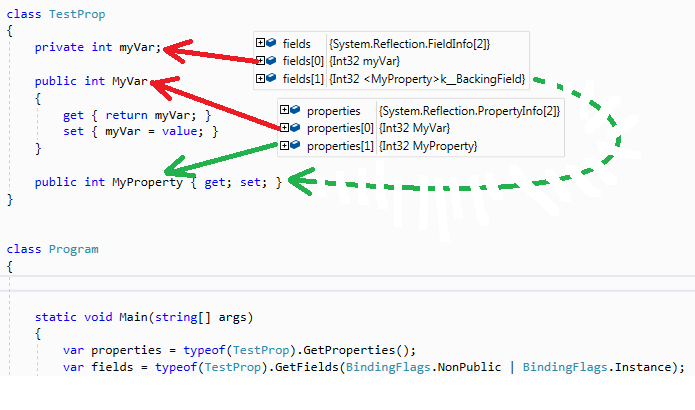
\includegraphics[width=\textwidth]{img/property_backing_field.png}
\end{frame}



\begin{frame}[fragile]
\frametitle{Javism -- gettery a settery}
\vfill
\begin{noblock}
\begin{lstlisting}[basicstyle=\small]
// String - klíčové slovo "string"
// atribut - místo vlastnosti
private String name;

// metoda jako getter a setter místo vlastosti
public String getName() {
    return name;
}

public void setName(String name) {
    this.name = name;
}
\end{lstlisting}
\end{noblock}
\vfill
\begin{yesblock}
\begin{lstlisting}[basicstyle=\small]
// "string"
// veřejná vlastnost - začíná velkým písmenem
public string Name { get; set; }
\end{lstlisting}
\end{yesblock}
\vfill
\end{frame}


\begin{frame}[fragile]
\begin{bitemize}{Vytváření vlastností ve Visual Studiu}
\item vlastnosti lze velmi efektivně vytvářet pomocí připravených code-snippets
\item []
\item \lstinline|prop<TAB><TAB>| -- vytvoří automaticky implementovanou vlastnost (TAB - přepíná mezi jednotlivými editovatelnými částmi)
\item \lstinline|propg<TAB><TAB>| -- stejné jako předchozí, ale je nastaveno \lstinline|private set|
\item \lstinline|propfull<TAB><TAB>| -- vytvoří vlastnost a backing atribut pro ní
\item \lstinline|propdp<TAB><TAB>| -- dependency property
\item \lstinline|propa<TAB><TAB>| -- attached dependency property
\end{bitemize}
\end{frame}


\kapitola{Metody}


\begin{frame}[fragile]
\frametitle{Metody}
\vfill
\begin{noteblock}{}
\begin{lstlisting}
[viditelnost] [modifikátory] typNávratovéHodnoty názevMetody([parametry]) těloMetody

těloMetody:
	=> výraz
	{ [příkazy] }
\end{lstlisting}
\end{noteblock}
\vfill
\begin{bitemize}{Modifikátory}
\item \lstinline|static| -- statická metoda
\item \lstinline|new| -- zakrývání metody z předka
\item \lstinline|virtual| -- virtuální metoda (polymorfizmus)
\item \lstinline|override| -- přetížená metoda (polymorfizmus)
\item \lstinline|abstract| -- abstraktní metoda (polymorfizmus)
\item \lstinline[morekeywords=async]|async| -- asynchronní metody
\end{bitemize}
\vfill
\end{frame}



\begin{frame}[fragile]
\frametitle{Metody -- příklad}
\vfill
\begin{yesblock}
\begin{lstlisting}[basicstyle=\small]
class Student
{
    public string Name { get; set; }

    public void SayHello()
    {
        Console.WriteLine($"Hello, I'm {Name}");
    }
}
\end{lstlisting}
\end{yesblock}
\vfill
\begin{yesblock}
\begin{lstlisting}[basicstyle=\small]
Student peter = new Student()
{
    Name = "Peter"
};

peter.SayHello();
\end{lstlisting}
\end{yesblock}
\vfill
\end{frame}




\begin{frame}[fragile]
\frametitle{Metody -- příklad zkráceného zápisu}
\vfill
\begin{yesblock}
\begin{lstlisting}[basicstyle=\small]
class Student
{
    public string Name { get; set; }

    public void SayHello() => Console.WriteLine($"Hello, I'm{Name}");
}
\end{lstlisting}
\end{yesblock}
\vfill
\end{frame}




\begin{frame}[fragile]
\frametitle{Metody -- výchozí hodnota parametru}
\begin{bitemize}{}
\item parametry mohou mít uvedenou výchozí hodnotu
\end{bitemize}
\vfill
\begin{yesblock}
\begin{lstlisting}[basicstyle=\small]
class MyMath
{
    public const double Pi = 3.141592;

    public static double GetPowerOfPi(int power = 1)
    {
        return Math.Pow(Pi, power);
    }
}
\end{lstlisting}
\end{yesblock}
\vfill
\begin{yesblock}
\begin{lstlisting}[basicstyle=\small]
double pi = MyMath.GetPowerOfPi();
double piSquare = MyMath.GetPowerOfPi(2);
\end{lstlisting}
\end{yesblock}
\end{frame}




\begin{frame}[fragile]
\frametitle{Metody -- ref}
\begin{bitemize}{}
\item parametr je možné předat odkazem (referencí)
\begin{itemize}
\item u parametru i u hodnoty argumentu je nutné uvést \lstinline|ref|
\end{itemize}

\end{bitemize}
\vfill
\begin{yesblock}
\begin{lstlisting}[basicstyle=\small]
class Toolkit
{
    public static void Increment(ref int value)
    {
        value++;
    }
}
\end{lstlisting}
\end{yesblock}
\vfill
\begin{yesblock}
\begin{lstlisting}[basicstyle=\small]
int intValue = 0;
Toolkit.Increment(ref intValue);
Console.WriteLine($"{intValue}");
\end{lstlisting}
\end{yesblock}
\end{frame}



\begin{frame}[fragile]
\frametitle{Metody -- out}
\begin{bitemize}{}
\item parametr může být výstupní
\begin{itemize}
\item u parametru i u hodnoty argumentu je nutné uvést \lstinline|out|
\end{itemize}

\end{bitemize}
\vfill
\begin{yesblock}
\begin{lstlisting}[basicstyle=\small]
class AuthenticationService
{
    public static bool Authentize(string password, out string username)
    {
        if (password == "secr3tP4ssw0rd!")
        {
            username = "admin";
            return true;
        }

        username = null;
        return false;
    }
}
\end{lstlisting}
\end{yesblock}
\end{frame}

\begin{frame}[fragile]
\frametitle{Metody -- out}
\vfill
\begin{yesblock}
\begin{lstlisting}[basicstyle=\small]
string username;
if(AuthenticationService.Authentize("password", out username))
{
    Console.WriteLine($"Authenticated as {username}");
}
\end{lstlisting}
\end{yesblock}
\vfill
\begin{yesblock}
\begin{lstlisting}[basicstyle=\small]
// C# 7 - podporuje deklarovat proměnnou v místě volání
if(AuthenticationService.Authentize("password", out string username))
{
    Console.WriteLine($"Authenticated as {username}");
}
\end{lstlisting}
\end{yesblock}
\vfill
\end{frame}




\nezkouskove

\begin{frame}[fragile]
\frametitle{Metody -- params}
\begin{bitemize}{}
\item je možné volat metodu s libovolným počtem parametrů (stejného typu)
\begin{itemize}
\item předáváno jako parametr typu pole s mod. \lstinline|params|
\item \lstinline|params| parametr musí být uveden jako poslední v seznamu parametrů
\end{itemize}

\end{bitemize}
\vfill
\begin{yesblock}
\begin{lstlisting}[basicstyle=\small]
public static int SumArguments(params int[] arguments)
{
    int sum = 0;
    foreach (var item in arguments)
    {
        sum += item;
    }

    return sum;
}
\end{lstlisting}
\end{yesblock}
\vfill
\begin{yesblock}
\begin{lstlisting}[basicstyle=\small]
int result = Summer.SumArguments(10, 20, 30, 40, 50, 60, 70);
\end{lstlisting}
\end{yesblock}
\end{frame}





\begin{frame}[fragile]
\frametitle{Metody -- pojmenované argumenty}
\begin{bitemize}{}
\item při volání metody je možné specifikovat argumenty v libovolném pořadí, pokud je uveden jejich název
\begin{itemize}
\item zapisuje se jako: \lstinline|názevParametru: hodnota|
\end{itemize}

\end{bitemize}
\vfill
\begin{yesblock}
\begin{lstlisting}[basicstyle=\small]
public static void AddProduct(string productName, int count = 1, 
    double weight = 0, string description = "")
\end{lstlisting}
\end{yesblock}
\vfill
\begin{yesblock}
\begin{lstlisting}[basicstyle=\small]
AddProduct("Toy", 10, 1.2, "Kid's toy");
AddProduct("Toy", count: 10, weight: 1.2);
AddProduct("Toy", description: "Kid's toy", count: 10);
// od C# 7.2:
AddProduct(productName: "Toy", 10, description: "Kid's toy"); 
\end{lstlisting}
\end{yesblock}
\end{frame}




\begin{frame}[fragile]
\frametitle{Metody -- ref return}

\begin{bitemize}{}
\item z metody je možné vracet referenci (C\# 7, mod. \lstinline|ref|)
\end{bitemize}
\vfill
\begin{yesblock}
\begin{lstlisting}[basicstyle=\small]
public static ref int FindGreaterThan(int[] array, int condition)
{
    for (int i = 0; i < array.Length; i++)
        if (array[i] > condition)
            return ref array[i];

    throw new Exception("Not found");
}
\end{lstlisting}
\end{yesblock}
\vfill
\begin{yesblock}
\begin{lstlisting}[basicstyle=\small]
int[] array = { 1, 2, 5, 15, 32, 64 };
Console.WriteLine($"{string.Join(" ", array)}");
ref int value = ref FindGreaterThan(array, 10);
value += 100;
Console.WriteLine($"{string.Join(" ", array)}");
\end{lstlisting}
\end{yesblock}
\end{frame}





\begin{frame}[fragile]
\frametitle{Metody -- rozšiřující (extension) metody}

\begin{bitemize}{}
\item (statická) metoda se tváří jako (instanční) metoda jiné třídy
\begin{itemize}
\item rozšířená třída je uvedena jako první parametr metody s mod. \lstinline|this|
\item metoda se volá přímo nad objektem rozšířené třídy
\end{itemize}

\item poprvé masivně použito pro realizaci LINQ
\end{bitemize}
\vfill
\begin{yesblock}
\begin{lstlisting}[basicstyle=\small]
class Student
{
  public string Name { get; set; }
}

static class StudentExtension
{
  public static void SayHello(this Student student, string weather)
  {
    Console.WriteLine($"Hello, I'm {student.Name} and it's {weather}");
  }
}
\end{lstlisting}
\end{yesblock}
\end{frame}

\begin{frame}[fragile]
\frametitle{Metody -- rozšiřující (extension) metody}
\begin{yesblock}
\begin{lstlisting}[basicstyle=\small]
Student student = new Student()
{
    Name = "Peter"
};

student.SayHello("sunny");
//Hello, I'm Peter and it's sunny
\end{lstlisting}
\end{yesblock}
\end{frame}


\zkouskove
%\kapitola{Datové složky a operace}

\begin{frame}[fragile]
\frametitle{Viditelnost / přístupová práva}

\begin{bitemize}
\item 3 úrovně:
\begin{itemize}
\item \lstinline|public| -- přístupné všude
\item \lstinline|protected| -- přístupné z potomků
\item \lstinline|private| -- přístupné pouze z vnitřku třídy
\end{itemize}
\item výchozí hodnota:
\begin{itemize}
\item \lstinline|struct| -- \lstinline|public|
\item \lstinline|class| -- \lstinline|private|
\end{itemize}

\item změna viditelnosti:
\begin{itemize}
\item uvozuje se blok (\lstinline|viditelnost: ...|)
\item bloky se mohou opakovat, být zpřeházené
\end{itemize}
\end{bitemize}

\begin{bonusblock}{friend}
\begin{itemize}
\item přátelé třídy (\lstinline|friend|) mají přístup i k \lstinline|protected| a \lstinline|private| složkám
\end{itemize}
\end{bonusblock}
\end{frame}


\begin{frame}[fragile]
\frametitle{Viditelnost / přístupová práva}
\begin{yesblock}
\begin{lstlisting}
struct Pes {
// implicitní public: (platí pro struct)
// implicitní private: (platí pro class)

  string jmeno; // je public

private:
  int id; // je private
  int vek; // je private
 
protected:
  int pocetChlupu; // je protected

public:
  int pocetNohou; // je public
};
\end{lstlisting}
\end{yesblock}
\end{frame}

\pkapitola{Atributy (datové složky)}

\begin{frame}[fragile]
\frametitle{Atributy}

\begin{noteblock}{}
\begin{lstlisting}
[static] datovýTyp názevAtributu [inicializátor];
\end{lstlisting}
\end{noteblock}

\begin{bitemize}
\item \lstinline|static| -- statický atribut (váže se na třídu, ne na objekt)
\item \lstinline|[inicializátor]|\cpp{11} -- umožňuje nastavit výchozí hodnotu (nelze u~statických atributů)
\end{bitemize}

\begin{yesblock}
\begin{lstlisting}
  int pocetChlupu = 12345;  
  static int pocetPsu;
\end{lstlisting}
\end{yesblock}


\begin{bonusblock}{}
\begin{itemize}
\item Dále existují modifikátory: \lstinline|mutable|, \lstinline|volatile|
\end{itemize}
\end{bonusblock}
\end{frame}



\begin{frame}[fragile]
\frametitle{Statické atributy}
\begin{bitemize}
\item statické atributy potřebují vyhradit paměť a inicializovat -- v CPP souboru
\end{bitemize}

\begin{exampleblock}{PES.H}
\begin{lstlisting}
struct Pes {
  static int pocetPsu;
};
\end{lstlisting}
\end{exampleblock}

\begin{exampleblock}{PES.CPP}
\begin{lstlisting}
int Pes::pocetPsu = 0;
\end{lstlisting}
\end{exampleblock}

\end{frame}


\begin{frame}[fragile]
\frametitle{Statické atributy (použití)}
\begin{exampleblock}{MAIN.CPP}
\begin{lstlisting}
  Pes pes = PsiBouda::vytvorPsa();
  Pes::pocetPsu++;

  cout << "Pocet psu: " << Pes::pocetPsu;
\end{lstlisting}
\end{exampleblock}
\end{frame}

\pkapitola{Metody}


\begin{frame}[fragile]
\frametitle{Metody}

\begin{noteblock}{}
\begin{lstlisting}
deklaraceMetody:
[static] [virtual] datovýTypNávratovéHodnoty názevMetody([parametry]) [const] [override] [final] [noexcept];
\end{lstlisting}
\end{noteblock}

\begin{bitemize}
\item \lstinline|static| -- statická metoda (váže se na třídu, ne na objekt)
\item \lstinline|virtual| -- virtuální metoda (polymorfizmus)
\item \lstinline|const| -- konstantní metoda (nemění stav objektu)
\item \lstinline|override|\cpp{11} -- označuje přetíženou metodu z předka (polymorfizmus)
\item \lstinline|final|\cpp{11} -- zakazuje další přepisování metody v potomcích
\item \lstinline|noexcept|\cpp{11} -- označuje metodu, která nevyvolává výjimky
\end{bitemize}
\end{frame}

\begin{frame}[fragile]
\frametitle{Metody\ldots}
\begin{bonusblock}{}
\begin{itemize}
\item modifikátor \lstinline|inline| -- optimalizace, nevolá funkci, vkládá kód přímo na místo volání; kompilátor dosadí automaticky, pokud je metoda definována uvnitř třídy
\item modifikátor \lstinline|volatile| -- nestálé metody
\item \lstinline|deklaraceMetody = delete;| -- C++11, smazání metody
\item \lstinline|deklaraceMetody = default;| -- C++11, vynucení implementace metody kompilátorem
\end{itemize}
\end{bonusblock}
\end{frame}


\begin{frame}[fragile]
\frametitle{Deklarace a definice metody uvnitř třídy}
\begin{yesblock}
\begin{lstlisting}
struct Pes {
  // deklarace - úplný funkční prototyp, bez těla
  void stekej();

  // definice - deklarace + tělo
  void kousej(Osoba& osoba) {
    osoba.zran(KOUSNUTI_DO_KOTNIKU);    
  }
};
\end{lstlisting}
\end{yesblock}
\end{frame}


\begin{frame}[fragile]
\frametitle{Deklarace a definice metody vně třídy}
\begin{bitemize}
\item definice metody vně třídy musí specifikovat, že jde o metodu dané třídy
\begin{itemize}
\item používá se operátor ::
\item uvádějí se pouze modifikátory \lstinline|const|, \lstinline|override|, \lstinline|noexcept|
\end{itemize}
\end{bitemize}
\begin{yesblock}
\begin{lstlisting}
struct Pes {
  // deklarace
  void kousej(Osoba& osoba);
};

// definice
void Pes::kousej(Osoba& osoba) {
  osoba.zran(KOUSNUTI_DO_KOTNIKU);   
}
\end{lstlisting}
\end{yesblock}
\end{frame}


\begin{frame}[fragile]
\frametitle{Metody a this}

\begin{bitemize}
\item uvnitř instančních metod je dostupný ukazatel \lstinline|this| (odpovídá \lstinline|Třída*|)
\begin{itemize}
\item není potřeba, implicitně je možné se odkazovat na složky třídy
\end{itemize}
\end{bitemize}

\begin{yesblock}
\begin{lstlisting}
struct Pes {
  void obnovZdravi() {
    // this je Pes*, následující výrazy jsou totožné
    _zdravi = 100;
    this->_zdravi = 100;
    (*this)._zdravi = 100;
  }

private:
  int _zdravi;
};
\end{lstlisting}
\end{yesblock}
\end{frame}


\pkapitola{Speciální metody}

\begin{frame}
\frametitle{Speciální metody}
\begin{block}{}
Existuje několik speciálních metod souvisejících s vytvářením a rušením objektů:
\begin{itemize}
\item konstruktory (bez parametrů, s parametry, kopírovací, konverzní, move)
\item destruktor
\item operátor =
\end{itemize}
Základní verzi těchto metod nám vytvoří automaticky kompilátor, pokud některou z metod nadefinujeme sami, kompilátor pak nemusí nic vytvářet (chybějící bezparametrický konstruktor).
\end{block}
\end{frame}


\begin{frame}[fragile]
\frametitle{Vznik a zánik objektu}
\begin{block}{}
\lstinline|struct Pes| dědí z (\lstinline|struct Zvire| dědí z (\lstinline|struct Objekt|))
\end{block}

\begin{block}{Proces vzniku a zániku objektu Pes}
\begin{itemize}
\item konstruktor \lstinline|Objekt|
\item konstruktor \lstinline|Zvire|
\item konstruktor \lstinline|Pes|
\item[]
\begin{itemize}
\item objekt žije, lze volat metody\ldots
\end{itemize}

\item destruktor \lstinline|Pes|
\item destruktor \lstinline|Zvire|
\item destruktor \lstinline|Objekt|
\end{itemize}
\end{block}
\end{frame}








\begin{frame}[fragile]
\frametitle{Konstruktor}
\begin{noteblock}{}
\begin{lstlisting}
názevTřídy([parametry]) [inicializačníČást];

inicializačníČást:
 : atribut1(hodnota1), ...
\end{lstlisting}
\end{noteblock}

\begin{bitemize}
\item nemá návratovou hodnotu (ani \lstinline|void|)!
\item inicializační část -- pro inicializaci datových složek
\begin{itemize}
\item je potřeba pro inicializaci referenčních atributů
\end{itemize}
\end{bitemize}

\begin{bonusblock}{}
\begin{itemize}
\item modifikátor \lstinline|explicit| -- zakazuje implicitní konverze
\end{itemize}
\end{bonusblock}
\end{frame}


\begin{frame}[fragile]
\frametitle{Bezparametrický konstruktor}
\begin{yesblock}
\begin{lstlisting}
struct Pes {

  Pes() {
    cout << "konstruktor Pes()" << endl;
  }

};
\end{lstlisting}
\end{yesblock}
\end{frame}


\begin{frame}[fragile]
\frametitle{Parametrický konstruktor}
\begin{yesblock}
\begin{lstlisting}
struct Pes {

  Pes(int zdravi) {
    cout << "konstruktor Pes(int)" << endl;
    _zdravi = zdravi;
  }

private:
  int _zdravi;
};
\end{lstlisting}
\end{yesblock}
\end{frame}




\begin{frame}[fragile]
\frametitle{Parametrický konstruktor s inicializační částí}
\begin{yesblock}
\begin{lstlisting}
struct Pes {

  Pes(int zdravi) : _zdravi(zdravi) {
    cout << "konstruktor Pes(int)" << endl;
  }

private:
  int _zdravi;
};
\end{lstlisting}
\end{yesblock}
\end{frame}



\begin{frame}[fragile]
\frametitle{Kopírovací konstruktor}
\begin{bitemize}
\item kompilátor ho umí vytvořit automaticky
\begin{itemize}
\item vytváří mělkou kopii (\lstinline|memcpy(kopie, original, sizeof(Typ))|)
\end{itemize}
\end{bitemize}
\begin{yesblock}
\begin{lstlisting}
struct Pes {

  Pes(const Pes& pes) {
    cout << "konstruktor Pes(const Pes&)" << endl;
    _zdravi = pes._zdravi;
  }

private:
  int _zdravi;
};
\end{lstlisting}
\end{yesblock}
\end{frame}





\begin{frame}[fragile]
\frametitle{Delegování konstruktorů\cpp{11}}
\begin{bonusblock}{}
\begin{itemize}
\item delegování umožňuje zavolat jiný konstruktor před vlastním vykonáním konstruktoru (od C++11)
\item inicializační část pak musí obsahovat pouze volání delegovaného konstruktoru!
\end{itemize}
\end{bonusblock}
\vskip -2ex
\begin{bonusblock}{}
\begin{lstlisting}[basicstyle=\scriptsize]
struct Pes {
  Pes(std::string jmeno) : _jmeno(pes,_jmeno) { 
    cout << "konstruktor Pes(std::string)" << endl;
  }

  Pes(std::string jmeno, int vek) : Pes(jmeno) {
    cout << "konstruktor Pes(std::string, int)" << endl;
    _vek = vek;
  }

private:
  std::string _jmeno;
  int _vek;
};
\end{lstlisting}
\end{bonusblock}
\end{frame}



\begin{frame}[fragile]
\frametitle{operátor =}
\begin{bonusblock}{}
\begin{itemize}
\item \lstinline|operator=| přepíše obsah objektu jiným objektem
\begin{itemize}
\item kompilátor vytváří automaticky
\item funguje na stejném principu jako kopírovací konstruktor
\end{itemize}
\end{itemize}
\end{bonusblock}
\vskip -2ex
\begin{bonusblock}{}
\begin{lstlisting}[basicstyle=\small]
struct Pes {
  Pes& operator=(const Pes& pes) {
    if (this == &pes)
      return *this;

    _jmeno = pes._jmeno;
    return *this;
  }

private:
  std::string _jmeno;
};
\end{lstlisting}
\end{bonusblock}
\end{frame}




\begin{frame}[fragile]
\frametitle{Move konstruktor\cpp{11}}
\begin{bonusblock}{}
\begin{itemize}
\item C++11 zavedlo novou \uv{move} sémantiku, funguje jako optimalizace, umožňuje převzít data z dočasných objektů
\begin{itemize}
\item R-value reference (\lstinline|Typ&&|)
\item move konstruktor (\lstinline|Typ(Typ&&))|)
\item move assignment operátor (\lstinline|operator=(Typ&&)|)
\end{itemize}
\end{itemize}
\end{bonusblock}
\vskip -2ex
\begin{bonusblock}{}
\begin{lstlisting}[basicstyle=\small]
struct Pes {

  Pes(Pes&& pes) : _jmeno(std::move(pes._jmeno)) {
    cout << "konstruktor Pes(Pes&&)" << endl;
  }

private:
  std::string _jmeno;
};
\end{lstlisting}
\end{bonusblock}
\end{frame}







\begin{frame}[fragile]
\frametitle{Destruktor}
\begin{noteblock}{}
\begin{lstlisting}
[virtual] ~názevTřídy();
\end{lstlisting}
\end{noteblock}

\begin{bitemize}
\item nemá návratovou hodnotu (ani \lstinline|void|)!
\item \lstinline|virtual| -- je potřeba při využívání polymorfizmu a dědičnosti!
\end{bitemize}

\begin{yesblock}
\begin{lstlisting}
struct Pes {
  ~Pes() {
    cout << "destruktor Pes()" << endl;
  }
};
\end{lstlisting}
\end{yesblock}
\end{frame}

%\hkapitola{Vytváření objektů}

\begin{frame}[fragile]
\begin{block}{Vytváření objektů}
\begin{itemize}
\item Staticky alokované objekty (\uv{statické objekty})
\begin{itemize}
\item na stacku (lokální proměnné, parametry funkcí)
\item globální prostor
\item statické atributy tříd

\end{itemize}
\item Dynamicky alokované objekty
\begin{itemize}
\item new, delete
\end{itemize}

\end{itemize}
\end{block}
\end{frame}

\kapitola{Staticky alokované objekty}

\begin{frame}
\begin{block}{Staticky alokované objekty}
\begin{itemize}
\item vytváří a ruší je kompilátor
\begin{itemize}
\item destruktor volá kompilátor!
\end{itemize}
\item životnost 
\begin{itemize}
\item do konce bloku (lokální proměnné, parametry)
\item do konce programu (globální proměnné, statické atributy tříd)
\end{itemize}
\end{itemize}
\end{block}
\end{frame}


\begin{frame}[fragile]
\frametitle{Vytváření statických objektů}

\begin{yesblock}
\begin{lstlisting}
void main() {
  // bezparametrický konstruktor
  Pes rafan;
  // parametrický konstruktor
  Pes kousak("Kousak", 200);

  // kopírovací konstruktor
  Pes kopieKousaka(kousak);
  Pes jinaKopieKousaka = kousak;
  // operátor=
  jinaKopieKousaka = kousak;
}
\end{lstlisting}
\end{yesblock}
\end{frame}


\begin{frame}[fragile]
\frametitle{Vytváření statických objektů\ldots}
\begin{noblock}
\begin{lstlisting}
// NELZE -> jedná se o deklaraci funkce!
// funkce vracející objekt Pes, bez parametrů
Pes rafan(); 

// lze, ale nevhodné -> může vést k vytvoření dočasného objektu a kopírování
Pes kousak = Pes("Kousak", 200);

// lze, ale nevhodné -> dochází k dvojímu volání destruktoru, dojde ke zničení VMT tabulky -> přestává fungovat polymorfizmus
kousak.~Pes();
\end{lstlisting}
\end{noblock}
\end{frame}



\begin{frame}[fragile]
\frametitle{Uniform initialization\cpp{11}}
\begin{bitemize}
\item C++11
\item použití pomocí složených závorek
\item volá konstruktor nebo inicializuje veřejné datové složky
\item jednotná syntaxe u všech případů!
\end{bitemize}

\begin{yesblock}
\begin{lstlisting}
void main() {
  // bezparametrický konstruktor
  Pes rafan{};
  // parametrický konstruktor
  Pes kousak{"Kousak", 200};
  // kopie
  Pes kopieKousaka{kousak};
}
\end{lstlisting}
\end{yesblock}
\end{frame}


\pkapitola{Volání funkcí -- předávání parametrů, návratová hodnota}


\begin{frame}[fragile]
\frametitle{Parametry funkcí}

\begin{yesblock}
\begin{lstlisting}
void funkce(Pes pes) {
  pes.stekej();
}

Pes rafan{};
// dojde k vytvoření kopie (kopírovací konstruktor)
// &pes != &rafan
funkce(rafan);
\end{lstlisting}
\end{yesblock}
\end{frame}


\begin{frame}[fragile]
\frametitle{Parametry funkcí (reference)}
\begin{bitemize}
\item Reference = předání odkazem
\begin{itemize}
\item \uv{Ukazatelem na pozadí}
\end{itemize}
\end{bitemize}

\begin{yesblock}
\begin{lstlisting}
void funkce(Pes& pes) {
  pes.stekej();
}

Pes rafan{};
// objekt je předán odkazem
// &pes == &rafan
funkce(rafan);
\end{lstlisting}
\end{yesblock}
\end{frame}


\begin{frame}[fragile]
\frametitle{Parametry funkcí (ukazatel)}

\begin{yesblock}
\begin{lstlisting}
void funkce(Pes* pes) {
  pes->stekej();

  // nezmění objekt, ani proměnné rafan a ptr
  // změní pouze lokální proměnnou pes
  pes = 0xdeadbeef;
}

Pes rafan{};
// objekt je předán pomocí ukazatele (je vytvořena kopie "Pes*" = 4(8) bajtové číslo - adresa v paměti)
Pes* ptr = &rafan;
// ptr == &rafan
funkce(ptr);
// ptr == &rafan
\end{lstlisting}
\end{yesblock}
\end{frame}




\begin{frame}[fragile]
\frametitle{Parametry funkcí (ukazatel na ukazatel)}

\begin{yesblock}
\begin{lstlisting}
void funkce(Pes** pes) {
  (*pes)->stekej();

  // nezmění objekt, ani proměnnou rafan
  // změní ukazatel ptr
  *pes = 0xdeadbeef;
}

Pes rafan{};
// objekt je předán pomocí ukazatele (je vytvořena kopie "Pes*" = 4(8) bajtové číslo - adresa v paměti)
Pes* ptr = &rafan;
// ptr == &rafan
funkce(&ptr);
// ptr == 0xdeadbeef
\end{lstlisting}
\end{yesblock}
\end{frame}



\begin{frame}[fragile]
\frametitle{Návratová hodnota}
\begin{bitemize}
\item Vrácení staticky alokovaného objektu vede ke kopírování
\begin{itemize}
\item Normálně se ale využije RVO (return value optimalization -- optimalizace kompilátorem)
\item Standard C++17 definuje \uv{Guaranteed copy elision} (= RVO ve standardu)
\end{itemize}
\end{bitemize}
\vskip -1ex
\begin{yesblock}
\begin{lstlisting}
Pes funkce() {
  Pes rafan{};
  return rafan;
  // objekt rafan - zaniká, ven jde kopie
}

// pes je vytvořen pomocí kopírovacího konstruktoru
// RVO -> kopírování nemusí nastat, objekt je předán "celý"
Pes pes = funkce();

\end{lstlisting}
\end{yesblock}
\end{frame}


\begin{frame}[fragile]
\frametitle{Návratová hodnota (reference)}
\begin{block}{}
Referenci lze vracet, pokud objekt nadále existuje
\begin{itemize}
\item je dynamicky alokovaný
\item je static (pozor u vícevláknových programů)
\item je na globálním prostoru (dtto)
\end{itemize}
\end{block}


\begin{yesblock}
\begin{lstlisting}
Pes& funkce() {
  Pes* rafan = new Pes{};
  return *rafan;
  // dynamicky alokovaný objekt je platný, dokud nezavoláme delete
}

// ok, ale pozor na memory leak!
Pes& pes = funkce();

\end{lstlisting}
\end{yesblock}
\end{frame}



\begin{frame}[fragile]
\frametitle{Návratová hodnota (reference)}
\begin{bitemize}
\item Návratový typ -- reference  + staticky alokovaný lokální objekt => nefunguje
\end{bitemize}

\begin{noblock}
\begin{lstlisting}
Pes& funkce() {
  Pes rafan{};
  return rafan;
  // objekt rafan - zaniká, ven jde zmetek!
}

// pes ukazuje na rozbitou paměť!
Pes& pes = funkce();

// MSVC obsahuje rozšíření, které daný příklad korektně provede, my pojedeme dle standardu C++ a nebudeme na to spoléhat
\end{lstlisting}
\end{noblock}
\end{frame}







\begin{frame}[fragile]
\frametitle{Návratová hodnota (reference)}

\begin{bonusblock}{Prodloužení životnosti dočasných objektů}
\begin{itemize}
\item Standard C++ umožňuje prodloužit životnost objektu v návratové hodnotě
\begin{itemize}
\item pro konstantní L-reference
\item pro R-reference
\end{itemize}
\end{itemize}
\end{bonusblock}

\begin{bonusblock}{}
\begin{lstlisting}
const Pes& funkce() {
  Pes rafan;
  return rafan;
}

// ok - uplatněno prodloužení životnosti objektu dle standardu
const Pes& pes = funkce();

\end{lstlisting}
\end{bonusblock}
\end{frame}


\kapitola{Dynamicky alokované objekty}

\begin{frame}
\begin{block}{Dynamicky alokované objekty}
\begin{itemize}
\item Vznikají a zanikají na náš explicitní příkaz (new / delete)
\end{itemize}
\end{block}
\end{frame}


\begin{frame}[fragile]
\frametitle{Objekt}
%\begin{bitemize}
%\item Objekt
%\end{bitemize}

\begin{yesblock}
\begin{lstlisting}
// vytvoření proměnné typu ukazatel
Pes* rafan = nullptr;
// alokace paměti, volání konstruktoru
rafan = new Pes{};

rafan->stekej();
(*rafan).stekej();

// volání destruktoru, dealokace paměti
delete rafan;
\end{lstlisting}
\end{yesblock}
\end{frame}



\begin{frame}[fragile]
\frametitle{Pole objektů}
%\begin{bitemize}
%\item Pole objektů
%\end{bitemize}

\begin{yesblock}
\begin{lstlisting}
// vytvoření proměnné typu ukazatel
Pes* rafani = nullptr;
// alokace paměti (5 * sizeof(Pes)), 5x volání konstruktoru
rafani = new Pes[5];

rafani[0].stekej();
(rafani + 0)->stekej();
(*(rafani + 0)).stekej();

// volání destruktorů (5x), dealokace paměti
delete[] rafani;
\end{lstlisting}
\end{yesblock}
\end{frame}


\begin{frame}[fragile]
\frametitle{Pole ukazatelů na objekt}
%\begin{bitemize}
%\item Pole ukazatelů na objekt
%\end{bitemize}

\begin{yesblock}

\begin{lstlisting}[basicstyle=\small]
Pes** rafani = nullptr;
rafani = new Pes*[5]; // alokace paměti (5 * sizeof(Pes*)), nevolá konstruktor!

for (int i = 0; i < 5; i++) 
  rafani[i] = new Pes{}; // alokace paměti objektu, konstruktor

rafani[0]->stekej();
(*rafani[0]).stekej();
(**(rafani+0)).stekej();

for (int i = 0; i < 5; i++) 
  delete rafani[i]; // destruktory, dealokace paměti objektů

delete[] rafani; // dealokace paměti pole
\end{lstlisting}
\end{yesblock}
\end{frame}



\begin{frame}[fragile]
\begin{oldblock}
\begin{itemize}
\item malloc, free -- neumí volat konstruktor a destruktor
\begin{itemize}
\item nepoužívejte je
\end{itemize}
\end{itemize}
\end{oldblock}

\begin{deprecatedblock}{}
\begin{lstlisting}[basicstyle={\small},commentstyle={\dcc}]
// vytvoření proměnné typu ukazatel
Pes* rafan = nullptr;
// alokace paměti
rafan = (Pes*)malloc(sizeof(Pes));
// konstrukce
new(rafan) Pes;

// ...

// destrukce
rafan->~Pes();
// uvolnění paměti
free(rafan);
rafan = nullptr;
\end{lstlisting}
\end{deprecatedblock}
\end{frame}




\begin{frame}[fragile]
\begin{noblock}{}
%[basicstyle={\small},commentstyle={\dcc}]
\begin{lstlisting}
// nekorektní kombinace new-delete[] / new[]-delete
Pes* pes = new Pes;
delete[] pes;

pes = new Pes[2];
delete pes;
\end{lstlisting}
\end{noblock}

\begin{noblock}{}
\begin{lstlisting}
// dvojí volání destruktoru
Pes* pes = new Pes;

pes->~Pes();
delete pes;
\end{lstlisting}
\end{noblock}
\end{frame}

%\kapitola{Konstatní a nekonstantní objekty}

\begin{frame}[fragile]
\begin{bitemize}
\item Nekonstantní objekt -- lze měnit jeho stav (atributy)
\item Konstantní objekt -- nelze měnit jeho stav (atributy)
\end{bitemize}


\begin{bitemize}
\item Nekonstantní metoda
\begin{itemize}
\item \lstinline|this| odpovídá typu \lstinline|Třída*|
\item může měnit stav
\end{itemize}

\item Konstantní metoda (za názvem \lstinline|const|)
\begin{itemize}
\item \lstinline|this| odpovídá typu \lstinline|const Třída*|
\item nemůže měnit stav
\end{itemize}
\end{bitemize}
\end{frame}




\begin{frame}[fragile]
\begin{bitemize}
\item Nekonstantní objekt
\begin{itemize}
\item Umí všechno!
\end{itemize}
\end{bitemize}

\begin{twocols}
\begin{yesblock}
\begin{lstlisting}[basicstyle=\small]
struct Pes {

  void stekej() { 
    cout << "Haf"; 
    _stekano = true; 
  };

  bool byloStekano() const { 
    return _stekano; 
  }

private:
  bool _stekano = false;
}
\end{lstlisting}
\end{yesblock}

\twocolssep

\begin{yesblock}
\begin{lstlisting}[basicstyle=\small]
Pes pes{};

pes.stekej();
cout << pes.byloStekano();
\end{lstlisting}
\end{yesblock}

\end{twocols}
\end{frame}




\begin{frame}[fragile]
\begin{bitemize}
\item Konstantní objekt -- neměnný
\begin{itemize}
\item Lze volat jen const metody!
\end{itemize}
\end{bitemize}

\begin{twocols}
\begin{yesblock}
\begin{lstlisting}[basicstyle=\small]
struct Pes {

  void stekej() { 
    cout << "Haf"; 
    _stekano = true; 
  };

  bool byloStekano() const { 
    return _stekano; 
  }

private:
  bool _stekano = false;
}
\end{lstlisting}
\end{yesblock}

\twocolssep

\begin{noblock}
\begin{lstlisting}[basicstyle=\small]
const Pes pes{};

pes.stekej(); // nejde
\end{lstlisting}
\end{noblock}

\begin{yesblock}
\begin{lstlisting}[basicstyle=\small]
const Pes pes{};

//pes.stekej(); - nejde
cout << pes.byloStekano();
\end{lstlisting}
\end{yesblock}

\end{twocols}
\end{frame}




\begin{frame}[fragile]
\frametitle{Více pohledů na jeden objekt\ldots}

\begin{yesblock}
\begin{lstlisting}
Pes pes{};

Pes& nekonstRefPes = pes;
nekonstRefPes.stekej();

const Pes& konstRefPes = pes;
// konstRefPes.stekej(); - nejde

Pes* nekonstPtrPes = &pes;
nekonstPtrPes->stekej();

const Pes* konstPtrPes = &pes;
// konstPtrPes->stekej(); - nejde
\end{lstlisting}
\end{yesblock}

\end{frame}








\begin{frame}[fragile]
\frametitle{Není const jako const\ldots}
\begin{yesblock}
\begin{lstlisting}
struct Pes {

  // nekonstatní metoda, vrací int
  int stekej1();

  // nekonstatní metoda, vrací const int
  const int stekej2();

  // konstatní metoda, vrací int
  int stekej3() const;

  // konstatní metoda, vrací const int
  const int stekej4() const;
}
\end{lstlisting}
\end{yesblock}
\end{frame}



\begin{frame}[fragile]
%\frametitle{Není const jako const (pokračování)\ldots}
\begin{bonusblock}{konstantní ukazatel}
\begin{itemize}
\item \lstinline|const| u ukazatele může značit konstantní ukazatel (neplést s~konstantním objektem)
\end{itemize}
\end{bonusblock}

\begin{bonusblock}{}
\begin{lstlisting}[basicstyle=\small]
// ukazatel na konstantní objekt
const Pes* pes1 = &pes;
// pes1->stekej() // NE
pes1 = nullptr; // OK

// konstantní ukazatel na nekonstantní objekt
Pes* const pes2 = &pes;
pes2->stekej() // OK
// pes2 = nullptr; // NE

// konstantní ukazatel na konstantní objekt
const Pes* const pes3 = &pes;
// pes3->stekej() // NE
// pes3 = nullptr; // NE
\end{lstlisting}
\end{bonusblock}
\end{frame}








\begin{frame}[fragile]
\begin{bonusblock}{mutable, volatile, constexpr, const\_cast}
\begin{itemize}
\item modifikátor \lstinline|mutable| (pro atributy)
\begin{itemize}
\item umožňuje měnit stav této proměnné i v konstantním objektu
\item odporuje obvyklé logice -- nebudeme používat
\end{itemize}

\item modifikátor \lstinline|volatile| (pro proměnné, atributy)
\begin{itemize}
\item \uv{nestálé instance} -- zakazuje optimalizace
\item stejný efekt jako konstantní-nekonstantní objekty
\end{itemize}

\item modifikátor \lstinline|constexpr| (pro funkce, metody)
\begin{itemize}
\item C++11
\item označuje metody a funkce jako \uv{compile time constant}
\item lze je pak použít pro definici velikosti pole, šablonového parametru, \ldots
\end{itemize}

\item operátor \lstinline|const_cast|
\begin{itemize}
\item umožňuje odstraňovat \lstinline|const| a \lstinline|volatile| modifikátory
\item nehlídá, jestli je to korektní!
\end{itemize}
\end{itemize}
\end{bonusblock}
\end{frame}


% 03
%\hkapitola{Dědičnost}

\begin{frame}[fragile]
\frametitle{Dědičnost v C++}

\begin{bitemize}
\item podporována vícenásobná dědičnost
\begin{itemize}
\item třída může dědit z několika tříd
\end{itemize}
\item neexistují rozhraní
\begin{itemize}
\item ale existují abstraktní třídy
\item uzavřené (sealed/final) třídy
\end{itemize}
\item u zděděných složek (atributů a metod) lze ovlivnit viditelnost
\begin{itemize}
\item lze hromadně omezit přístup k těmto složkám
\item lze individuálně obnovit nebo omezit přístup
\end{itemize}
\item metody lze přetížit/přepsat v potomcích
\begin{itemize}
\item C++ rozlišuje časnou a pozdní vazbu
\end{itemize}
\end{bitemize}
\end{frame}


\begin{frame}[fragile]
\frametitle{Dědičnost}
\begin{noteblock}{}
\begin{lstlisting}[basicstyle=\scriptsize]
struct|class nazevDatovehoTypu [final] [dědičnost] {
  [složky - atributy, metody, vnořené typy]
} [objekty];
\end{lstlisting}
\end{noteblock}

\begin{bitemize}
\item{} [\lstinline|final|]\cpp{11} -- zakazuje dědit z této třídy
\item{} [dědičnost] -- specifikace předků
\begin{itemize}
\item \lstinline|: [viditelnost] [virtual] předek1, ...|
\end{itemize}
\end{bitemize}

\begin{yesblock}
\begin{lstlisting}
struct Pes : public virtual Zvire, public IIdentifikovatelny, IKopirovatelny {
  ...
};
\end{lstlisting}
\end{yesblock}
\end{frame}

\begin{frame}[fragile]
\frametitle{Dědičnost\ldots}
\begin{bitemize}
\item pokud viditelnost není uvedena využije se výchozí dle typu
\begin{itemize}
\item \lstinline|class| -- \lstinline|private|
\item \lstinline|struct| -- \lstinline|public|
\end{itemize}
\item viditelnost udává s jakou viditelností jsou zděděny složky z daného předka, pokud uvedeme
\begin{itemize}
\item \lstinline|public| -- nic se nemění
\item \lstinline|protected| -- \lstinline|public| složky z předka jsou převedeny na \lstinline|protected|
\item \lstinline|private| -- \lstinline|public| a \lstinline|protected| složky z předka jsou převedeny na \lstinline|private|
\end{itemize}
\end{bitemize}

\begin{noteblock}{}
Aby se to chovalo á la Java:
\begin{itemize}
\item používejte \lstinline|struct| a nic tam nepište
\item používejte \lstinline|struct| i \lstinline|class| a vždy uvádějte viditelnost \lstinline|public|
\end{itemize}
\end{noteblock}
\end{frame}






\begin{frame}[fragile]
\frametitle{Dědičnost\ldots}
\begin{bonusblock}{Obnovení viditelnosti}
\begin{itemize}
\item viditelnost je možné obnovit uvedením složky předka ve tvaru \lstinline|TřídaPředka::složka| v bloku s danou viditelností (rovněž lze využít i \lstinline|using TřídaPředka::složka|)
\end{itemize}
\end{bonusblock}
\vskip -2ex
\begin{bonusblock}{}
\begin{twocols}
\begin{lstlisting}
class TA {

  protected:
    int x, y;

  public:
    int GetX() const;
    // ...
};

\end{lstlisting}
\twocolssep
\begin{lstlisting}
class TB : private TA {

  protected:
    TA::x;

  public:
    TA::GetX;
    // ...
};
\end{lstlisting}
\end{twocols}
\end{bonusblock}
\end{frame}









\begin{frame}[fragile]
\begin{bitemize}
\item potomek může zastoupit předka
\begin{itemize}
\item je korektní přiřadit ukazatel na potomka do ukazatele na předka
\item je korektní přiřadit referenci na potomka do reference na předka
\item NENÍ korektní přiřadit objekt potomka do objektu předka
\begin{itemize}
\item dojde k oříznutí objektu!
\end{itemize}
\end{itemize}
\end{bitemize}

\begin{yesblock}
\begin{lstlisting}
Potomek potomek{};

Predek& ref = potomek;
Predek* ptr = &potomek;
...
\end{lstlisting}
\end{yesblock}

\begin{noblock}
\begin{lstlisting}
Predek predek = potomek; // oříznutí objektu!!!
\end{lstlisting}
\end{noblock}
\end{frame}







\begin{frame}[fragile]
\frametitle{Volání konstruktoru předka}

\begin{yesblock}
\begin{lstlisting}[basicstyle=\scriptsize]
struct Predek {
  Predek() : _a(0) { }
  Predek(int a) : _a(a) { }

private:
  int _a;
}

struct Potomek : Predek {
  Potomek() : _b(0) {
    // kompilátor implicitně volá Predek::Predek();
  }

  Potomek(int a, int b) : Predek(a), _b(0) {
    // kompilátor explicitně volá Predek::Predek(int);
  }

private:
  int _b;
}
\end{lstlisting}
\end{yesblock}
\end{frame}


\begin{frame}[fragile]
%\frametitle{Volání konstruktoru předka\ldots}
%\vskip -.99ex
\begin{yesblock}
\begin{lstlisting}[basicstyle=\scriptsize]
struct Predek {
  //Predek() : _a(0) { }
  Predek(int a) : _a(a) { }

private:
  int _a;
}
\end{lstlisting}
\end{yesblock}
%\vskip -2.0ex
\begin{noblock}
\begin{lstlisting}[basicstyle=\scriptsize]
struct Potomek : Predek {
  Potomek() : _b(0) {
    // kompilátor implicitně volá Predek::Predek();
    // konstruktor neexistuje !!! chyba kompilace
  }

  Potomek(int a, int b) : Predek(a), _b(0) {
    // kompilátor explicitně volá Predek::Predek(int);
    // ok!
  }

private:
  int _b;
}
\end{lstlisting}
\end{noblock}
\end{frame}




% virtualni nevirtualni dedeni
% using na konstruktory
% volani konstruktoru predka
% proces tvorby objektu?

%\hkapitola{Polymorfizmus}

\begin{frame}[fragile]
\begin{bitemize}
\item jedna funkce/metoda může nabývat více různých podob
\item metoda \lstinline|pracuj()| z rozhraní \lstinline|IPracujici|
\begin{itemize}
\item sekačka -- seká
\item policista -- uděluje pokuty
\item pes -- štěká
\end{itemize}
\end{bitemize}

\begin{noteblock}{Způsoby volání metod v C++}
\begin{itemize}
\item časná vazba -- výchozí, kompilátor řeší v době překladu
\item pozdní vazba -- na vyžádání (\lstinline|virtual|), řeší se v době vykonávání programu
\item []
\item Java -- automaticky vždy uplatňuje pozdní vazbu! chování v C++ a C\# je tedy odlišné
\end{itemize}
\end{noteblock}
\end{frame}







\begin{frame}[fragile]
\frametitle{Časná vazba}

\begin{yesblock}
\begin{twocols}
\begin{lstlisting}
struct Zvire {
  void vydejZvuk() {
    cout << "err";
  }
};
\end{lstlisting}

\twocolssep

\begin{lstlisting}
struct Kralik : Zvire {
  void vydejZvuk() {
    cout << "Bzzzm!";
  }
};
\end{lstlisting}
\end{twocols}
\end{yesblock}

\begin{yesblock}
\begin{lstlisting}
Zvire z{};
z.vydejZvuk(); // err

Kralik k{};
k.vydejZvuk(); // Bzzzm!
\end{lstlisting}
\end{yesblock}
\end{frame}







\begin{frame}[fragile]
\frametitle{Časná vazba\ldots}

\begin{yesblock}
\begin{twocols}
\begin{lstlisting}
struct Zvire {
  void vydejZvuk() {
    cout << "err";
  }
};
\end{lstlisting}

\twocolssep

\begin{lstlisting}
struct Kralik : Zvire {
  void vydejZvuk() {
    cout << "Bzzzm!";
  }
};
\end{lstlisting}
\end{twocols}
\end{yesblock}

\begin{noblock}
\begin{lstlisting}
Zvire& refz = k;
refz.vydejZvuk(); // err

Zvire* ptrz = &k;
ptrz->vydejZvuk(); // err
\end{lstlisting}
\end{noblock}
\end{frame}






\begin{frame}[fragile]
\frametitle{Pozdní vazba}

\begin{yesblock}
\begin{twocols}
\begin{lstlisting}
struct Zvire {
  virtual void vydejZvuk() {
    cout << "err";
  }
};
\end{lstlisting}

\twocolssep

\begin{lstlisting}
struct Kralik : Zvire {
  void vydejZvuk() {
    cout << "Bzzzm!";
  }
};
\end{lstlisting}
\end{twocols}
\end{yesblock}

\begin{yesblock}
\begin{lstlisting}
Zvire& refz = k;
refz.vydejZvuk(); // Bzzzm!

Zvire* ptrz = &k;
ptrz->vydejZvuk(); // Bzzzm!
\end{lstlisting}
\end{yesblock}
\end{frame}






\begin{frame}[fragile]
\frametitle{Pozdní vazba\ldots}

\begin{bitemize}
\item metoda musí být označena \lstinline|virtual| v předkovi
\item reference a ukazatele poté za běhu dohledají správnou metodu
\item využívá se VMT (virtual method table), kompilátor ji automaticky vytváří a vkládá na ni ukazatel do každého objektu
\end{bitemize}
\end{frame}





\begin{frame}[fragile]
\frametitle{Pozdní vazba\ldots}


\begin{yesblock}
\begin{twocols}
\begin{lstlisting}[basicstyle=\scriptsize]
struct Zvire {
  virtual void vydejZvuk() {
    cout << "err";
  }
};
\end{lstlisting}

\twocolssep

\begin{lstlisting}[basicstyle=\scriptsize]
struct Kralik : Zvire {
  void vydejZvuk() {
    cout << "Bzzzm!";
  }
};
\end{lstlisting}
\end{twocols}
\end{yesblock}

\vskip -3ex
\begin{yesblock}
\begin{twocols}
\begin{lstlisting}[basicstyle=\scriptsize]
struct Zvire {
  virtual void vydejZvuk() {
    cout << "err";
  }
};
\end{lstlisting}

\twocolssep

\begin{lstlisting}[basicstyle=\scriptsize]
struct Kralik : Zvire {
  virtual void vydejZvuk() {
    cout << "Bzzzm!";
  }
};
\end{lstlisting}
\end{twocols}
\end{yesblock}

\vskip -3ex
\begin{yesblock}
\begin{twocols}
\begin{lstlisting}[basicstyle=\small]
struct Zvire {
  virtual void vydejZvuk() {
    cout << "err";
  }
};
\end{lstlisting}

\twocolssep

\begin{lstlisting}[basicstyle=\small]
struct Kralik : Zvire {
  virtual void vydejZvuk() override {
    cout << "Bzzzm!";
  }
};
\end{lstlisting}
\end{twocols}
\end{yesblock}

\end{frame}





\begin{frame}[fragile]
\frametitle{Pozdní vazba\ldots}

\begin{block}{}
Doporučené použití:
\begin{itemize}
\item předek -- \lstinline|virtual|
\begin{itemize}
\item povinné, jinak nebude fungovat!
\end{itemize}
\item potomek -- \lstinline|virtual + override|
\begin{itemize}
\item \lstinline|virtual| -- pro přehlednost, že se jedná o virtuální metodu
\item \lstinline|override|\cpp{11} -- zajistí kontrolu kompilátorem, že předpis odpovídá virtuální metodě z předka
\end{itemize}
\end{itemize}
\end{block}
\end{frame}


\begin{frame}[fragile]
\frametitle{Pozdní vazba\ldots}

\begin{block}{}
Destruktor:
\begin{itemize}
\item časná/pozdní vazba se uplatňuje stejným způsobem na destruktor!
\begin{itemize}
\item aby bylo zajištěno, že se zavolá správný destruktor, musí být v předkovi virtuální destruktor
\item \textbf{každá třída ze které se dědí by měla mít virtuální destruktor}
\end{itemize}
\end{itemize}
\end{block}
\end{frame}



\begin{frame}[fragile]
\frametitle{Čistě virtuální metody}

\begin{bitemize}
\item virtuální metoda (\lstinline|virtual|) -- uplatnění pozdní vazby
\item čistě virtuální metoda (abstraktní, \lstinline|virtual ... = 0;|) -- pozdní vazba + chybí tělo (nutno doplnit v potomkovi)
\begin{itemize}
\item nelze vytvářet objekty od třídy obsahující čistě virtuální metody!
\end{itemize}
\end{bitemize}


\begin{yesblock}
\begin{lstlisting}
struct Zvire {
  virtual void vydejZvuk() = 0; // čistě virtuální / pure virtual
};

struct Kralik : Zvire {
  virtual void vydejZvuk() override {
    cout << "Bzzzm!";
  }
};

\end{lstlisting}
\end{yesblock}
\end{frame}





\begin{frame}[fragile]
\frametitle{Čistě virtuální metody\ldots}


\begin{noblock}
\begin{lstlisting}
struct Zvire {
  virtual void vydejZvuk() = 0; // čistě virtuální / pure virtual
};

Zvire z{}; // nelze - Zvire je abstraktní třída
\end{lstlisting}
\end{noblock}

\begin{bonusblock}{}
\begin{itemize}
\item čistě virtuální metoda může mít i tělo (definici)
\begin{itemize}
\item stále je pak čistě virtuální (abstraktní)
\item tělo lze explicitně volat z potomka \lstinline|Predek::cisteVirtualniMetoda()|
\end{itemize}
\end{itemize}
\end{bonusblock}
\end{frame}





\begin{frame}[fragile]
\frametitle{Rozhraní}

\begin{bitemize}
\item čistě virtuální metody lze použít pro realizaci typu \uv{rozhraní}
\begin{itemize}
\item nezapomínejte na virtuální destruktor!
\end{itemize}
\end{bitemize}


\begin{yesblock}
\begin{lstlisting}
struct IZvire {

  virtual ~IZvire() { }

  virtual void vydejZvuk() = 0;
  virtual void nakrm(Potravina* potravina) = 0;
  virtual void zautoc(IZvire* zvire) = 0;
};
\end{lstlisting}
\end{yesblock}
\end{frame}











%\nezkouskove
\section{Implementace dědičnosti v C++}

\begin{frame}[fragile]
\vskip 3cm
\begin{bonusblock}{}
\vskip 2ex
\Large \centering
Implementace dědičnosti v C++
\vskip 2ex
\end{bonusblock}
\vskip 1.5cm
\begin{center}
{\small Následující část přednášky obsahuje informace k bližšímu pochopení, jak interně funguje vícenásobná dědičnost a polymorfizmus. \\ Podrobně viz \url{ https://www.usenix.org/legacy/publications/compsystems/1989/fall_stroustrup.pdf}} \\ \textbf{Nejedná se o téma potřebné do zkoušky/zápočtu!}
\end{center}

\end{frame}


\begin{frame}[fragile]
\begin{bonusblock}{Objekt}
\begin{itemize}
\item objekt je spojitá část paměti, kde jsou uloženy atributy daného objektu
\item atributy jsou uloženy v pořadí dle pořadí definování
\item pokud třída dědí z jiné třídy $\rightarrow$ v paměti jsou v souvislém bloku uloženy hodnoty atributů ze všech předků i z dané třídy
\item[]
\item metoda je realizována jako vylepšená funkce
\begin{itemize}
\item na pozadí od kompilátoru obdrží ukazatel \lstinline|this|
\end{itemize}

\end{itemize}

\end{bonusblock}
\end{frame}

\begin{frame}[fragile]
\begin{bonusblock}{}
\vskip 2ex
\large \centering
Varianta A) Jednoduchá dědičnost
\vskip 2ex
\end{bonusblock}
\end{frame}



\begin{frame}[fragile]
\begin{noteblock}{}
\begin{twocols}
\begin{lstlisting}[basicstyle=\scriptsize]
struct A {
  int a = 0xaaaaaaaa;
  int b = 0xbbbbbbbb;

  int getA() const { return a; }
  int getB() const { return b; }
};
\end{lstlisting}
\twocolssep
\begin{lstlisting}[basicstyle=\scriptsize]
struct B : A {
  int c = 0xcccccccc;
  int d = 0xdddddddd;

  int getC() const { return c; }
  int getD() const { return d; }
};
\end{lstlisting}
\end{twocols}
\end{noteblock}


\begin{overlayarea}{\textwidth}{3cm}

\begin{threecols}

\begin{yesblock}<2->
\begin{lstlisting}
A objA{};
B objB{};
\end{lstlisting}
\end{yesblock}

\threecolssep

\centering
\only<3,4>{
\begin{tabular}{r|c|}
\hline
&	objA \\
\hline 
0x00 & \ttfamily 0xaaaaaaaa \\
\hline
0x04 & \ttfamily 0xbbbbbbbb \\
\hline
\end{tabular}
}\only<5>{
\begin{tabular}{r|cccc|}
\hline
\thisse & \multicolumn{4}{c|}{objA} \\
\hline 
\bc 0x00 & \bc aa & \bc aa & \bc aa & \bc aa \\
\hline
0x04 & bb & bb & bb & bb \\
\hline
\end{tabular}
}\only<6>{
\begin{tabular}{r|cccc|}
\hline
\thisse & \multicolumn{4}{c|}{objA} \\
\hline 
\gc 0x00 & \gc aa & \gc aa & \gc aa & \gc aa \\
\hline
\bc 0x04 & \bc bb & \bc bb & \bc bb & \bc bb \\
\hline
\end{tabular}
}\only<7>{
\begin{tabular}{r|cccc|}
\hline
\thisse & \multicolumn{4}{c|}{objB} \\
\hline 
\gc 0x00 & \gc aa & \gc aa & \gc aa & \gc aa \\
\hline
\gc 0x04 & \gc bb & \gc bb & \gc bb & \gc bb \\
\hline 
\bc 0x08 & \bc cc & \bc cc & \bc cc & \bc cc \\
\hline
0x0c & dd & dd & dd & dd \\
\hline
\end{tabular}
}\only<8>{
\begin{tabular}{r|cccc|}
\hline
\thisse & \multicolumn{4}{c|}{objB} \\
\hline 
\gc 0x00 & \gc aa & \gc aa & \gc aa & \gc aa \\
\hline
\gc 0x04 & \gc bb & \gc bb & \gc bb & \gc bb \\
\hline 
\gc 0x08 & \gc cc & \gc cc & \gc cc & \gc cc \\
\hline
\bc 0x0c & \bc dd & \bc dd & \bc dd & \bc dd \\
\hline
\end{tabular}
}

\threecolssep

\begin{overlayarea}{\textwidth}{3cm}
\centering
\only<4>{
\begin{tabular}{r|c|}
\hline
& objB \\
\hline 
0x00 & \ttfamily 0xaaaaaaaa \\
\hline
0x04 & \ttfamily 0xbbbbbbbb \\
\hline 
0x08 & \ttfamily 0xcccccccc \\
\hline
0x0c & \ttfamily 0xdddddddd \\
\hline
\end{tabular}
}
\end{overlayarea}

\end{threecols}
\end{overlayarea}


\begin{overlayarea}{\textwidth}{3cm}
\begin{onlyenv}<5>
\begin{yesblock}
\begin{lstlisting}
int get<@\color{red}A@>() const {
  return * (int*) ( ((char*)this) + <@\color{red}0x00@>);
}
\end{lstlisting}
\end{yesblock}
\end{onlyenv}

\begin{onlyenv}<6>
\begin{yesblock}
\begin{lstlisting}
int get<@\color{red}B@>() const {
  return * (int*) ( ((char*)this) + <@\color{red}0x04@>);
}
\end{lstlisting}
\end{yesblock}
\end{onlyenv}

\begin{onlyenv}<7>
\begin{yesblock}
\begin{lstlisting}
int get<@\color{red}C@>() const {
  return * (int*) ( ((char*)this) + <@\color{red}0x08@>);
}
\end{lstlisting}
\end{yesblock}
\end{onlyenv}

\begin{onlyenv}<8>
\begin{yesblock}
\begin{lstlisting}
int get<@\color{red}D@>() const {
  return * (int*) ( ((char*)this) + <@\color{red}0x0c@>);
}
\end{lstlisting}
\end{yesblock}
\end{onlyenv}
\end{overlayarea}

\end{frame}




\begin{frame}[fragile]
\begin{bonusblock}{}
\vskip 2ex
\large \centering
Varianta B) Vícenásobná dědičnost
\vskip 2ex
\end{bonusblock}
\end{frame}





\begin{frame}[fragile]

\begin{noteblock}{}
\begin{threecols}
\begin{lstlisting}[basicstyle=\scriptsize]
struct A {
  int a = 0xaaaaaaaa;
  int b = 0xbbbbbbbb;
  ...
};
\end{lstlisting}
\threecolssep
\begin{lstlisting}[basicstyle=\scriptsize]
struct B {
  int c = 0xcccccccc;
  int d = 0xdddddddd;
  ...
};
\end{lstlisting}
\threecolssep
\begin{lstlisting}[basicstyle=\scriptsize]
struct C : A, B {
  int e = 0xeeeeeeee;
  int f = 0xffffffff;
  ...
};
\end{lstlisting}
\end{threecols}
\end{noteblock}

\begin{overlayarea}{\textwidth}{4cm}
\begin{onlyenv}<2-7>
\begin{twocols}
\begin{yesblock}<2->
\begin{lstlisting}
C objC{};
\end{lstlisting}
\end{yesblock}

\twocolssep
\begin{overlayarea}{\textwidth}{4cm}
\begin{onlyenv}<3>
\begin{tabular}{r|c|l}
\hline
& objC & \\
\hline 
0x00 & \ttfamily 0xaaaaaaaa & $\leftarrow$ A \\
\hline
0x04 & \ttfamily 0xbbbbbbbb & \\
\hline 
0x08 & \ttfamily 0xcccccccc & $\leftarrow$ B \\
\hline
0x0c & \ttfamily 0xdddddddd & \\
\hline
0x10 & \ttfamily 0xeeeeeeee & $\leftarrow$ C \\
\hline
0x14 & \ttfamily 0xffffffff & \\
\hline
\end{tabular}
\end{onlyenv}\begin{onlyenv}<4>
\begin{tabular}{r|cccc|}
\hline
& \multicolumn{4}{c|}{objC} \\
\hline 
0x00 & aa & aa & aa & aa \\
\hline
0x04 & bb & bb & bb & bb \\
\hline 
0x08 & cc & cc & cc & cc \\
\hline
0x0c & dd & dd & dd & dd\\
\hline
0x10 & ee & ee & ee & ee\\
\hline
0x14 & ff & ff & ff & ff\\
\hline
\end{tabular}
\end{onlyenv}\begin{onlyenv}<5>
\begin{tabular}{r|cccc|}
\hline
\thisse & \multicolumn{4}{c|}{objC} \\
\hline 
\bc 0x00 & \bc aa & \bc aa & \bc aa & \bc aa \\
\hline
\bc 0x04 & \bc bb & \bc bb & \bc bb & \bc bb \\
\hline 
0x08 & cc & cc & cc & cc \\
\hline
0x0c & dd & dd & dd & dd\\
\hline
0x10 & ee & ee & ee & ee\\
\hline
0x14 & ff & ff & ff & ff\\
\hline
\end{tabular}
\end{onlyenv}\begin{onlyenv}<6>
\begin{tabular}{r|cccc|}
\hline
\thisse & \multicolumn{4}{c|}{objC} \\
\hline 
\rc 0x00 & \rc aa & \rc aa & \rc aa & \rc aa \\
\hline
\rc 0x04 & \rc bb & \rc bb & \rc bb & \rc bb \\
\hline 
0x08 & cc & cc & cc & cc \\
\hline
0x0c & dd & dd & dd & dd\\
\hline
0x10 & ee & ee & ee & ee\\
\hline
0x14 & ff & ff & ff & ff\\
\hline
\end{tabular}
\end{onlyenv}\begin{onlyenv}<7>
\begin{tabular}{r|cccc|}
\hline
\thisse & \multicolumn{4}{c|}{objC} \\
\hline 
0x00 & aa & aa & aa & aa \\
\hline
0x04 & bb & bb & bb & bb \\
\hline 
0x08 & cc & cc & cc & cc \\
\hline
0x0c & dd & dd & dd & dd\\
\hline
\bc 0x10 & \bc ee & \bc ee & \bc ee & \bc ee \\
\hline
\bc 0x14 & \bc ff & \bc ff & \bc ff & \bc ff \\
\hline
\end{tabular}
\end{onlyenv}
\end{overlayarea}
\end{twocols}
\end{onlyenv}\begin{onlyenv}<8>
\begin{block}{}
Původní předpoklad selhal u druhého předka v objektu objC\ldots
\begin{itemize}
\item reálná implementace ale funguje
\item kompilátor umí transformovat začátek objektu dle potřeby
\item \lstinline|(C*)&objC == (B*)&objC|
\item \lstinline|(char*)((C*)&objC) != (char*)((B*)&objC)|

\end{itemize}
Ve skutečnosti tedy\ldots
\end{block}
\end{onlyenv}\begin{onlyenv}<9>
\begin{center}
\vskip -5mm
\begin{tabular}{r|cccc|}
\hline
& \multicolumn{4}{c|}{objC} \\
\hline 
0x00 & aa & aa & aa & aa \\
\hline
0x04 & bb & bb & bb & bb \\
\hline 
\bc 0x08 \thise & \bc cc & \bc cc & \bc cc & \bc cc \\
\hline
\bc 0x0c & \bc dd & \bc dd & \bc dd & \bc dd\\
\hline
0x10 & ee & ee & ee & ee\\
\hline
0x14 & ff & ff & ff & ff\\
\hline
\end{tabular}
\end{center}
\end{onlyenv}
\end{overlayarea}

\begin{overlayarea}{\textwidth}{4cm}
\begin{onlyenv}<9>
\vskip -5mm
\begin{yesblock}
\begin{lstlisting}[basicstyle=\small]
int impl_getC_classC(C* object) {
  B* temporary = (B*)((char*)object + 0x08);
  return temporary->getC();
}
\end{lstlisting}
\end{yesblock}
\end{onlyenv}\begin{onlyenv}<5-7>
\begin{yesblock}
\begin{onlyenv}<5>
\begin{lstlisting}
get<@\color{red}A@>() -> * (int*) (((char*)this) + 0x00)
get<@\color{red}B@>() -> * (int*) (((char*)this) + 0x04)
\end{lstlisting}
\end{onlyenv}

\begin{onlyenv}<6>
\begin{lstlisting}
get<@\color{red}C@>() -> * (int*) (((char*)this) + 0x00)
get<@\color{red}D@>() -> * (int*) (((char*)this) + 0x04)
\end{lstlisting}
\end{onlyenv}

\begin{onlyenv}<7>
\begin{lstlisting}
get<@\color{red}E@>() -> * (int*) (((char*)this) + 0x10)
get<@\color{red}F@>() -> * (int*) (((char*)this) + 0x14)
\end{lstlisting}
\end{onlyenv}

\end{yesblock}
\end{onlyenv}
\end{overlayarea}


\end{frame}










\begin{frame}[fragile]
\begin{bonusblock}{}
\vskip 2ex
\large \centering
Varianta C) Diamond problem -- virtuální dědičnost
\vskip 2ex
\end{bonusblock}
\end{frame}








\begin{frame}[fragile]
\begin{noteblock}{}
\begin{lstlisting}
struct A {
  int a = 0xaaaaaaaa;
  int b = 0xbbbbbbbb;
};
\end{lstlisting}
\end{noteblock}

\begin{twocols}
\begin{noteblock}{}
\begin{lstlisting}
struct B : A {
  int c = 0xcccccccc;
  int d = 0xdddddddd;
}
\end{lstlisting}
\end{noteblock}
\twocolssep
\begin{noteblock}{}
\begin{lstlisting}
struct C : A {
  int e = 0xeeeeeeee;
  int f = 0xffffffff;
}
\end{lstlisting}
\end{noteblock}
\end{twocols}

\begin{noteblock}{}
\begin{lstlisting}
struct D : B, C {
  int x = 0x99999999;
}
\end{lstlisting}
\end{noteblock}
\end{frame}



\begin{frame}[fragile]
\begin{yesblock}
\begin{lstlisting}
D objD{};
\end{lstlisting}
\end{yesblock}

\vskip 1ex
\begin{center}
\begin{onlyenv}<1>
\begin{tabular}{c|c|l}
& objD & \\
\hline
0x00 & \ttfamily 0xaaaaaaaa & $\leftarrow B, A_B$ \\
\hline
0x04 & \ttfamily 0xbbbbbbbb & \\
\hline
0x08 & \ttfamily 0xcccccccc & $\leftarrow B\ldots$ \\
\hline
0x0c & \ttfamily 0xdddddddd &  \\
\hline
0x10 & \ttfamily 0xaaaaaaaa & $\leftarrow C, A_C$ \\
\hline
0x14 & \ttfamily 0xbbbbbbbb & \\
\hline
0x18 & \ttfamily 0xeeeeeeee & $\leftarrow C\ldots$ \\
\hline
0x1c & \ttfamily 0xffffffff &  \\
\hline
0x20 & \ttfamily 0x99999999 & $\leftarrow D$ \\
\hline
\end{tabular}
\end{onlyenv}\begin{onlyenv}<2>
\begin{tabular}{c|c|l}
& objD & \\
\hline
0x00 & \ttfamily \bc 0xaaaaaaaa & $\leftarrow B, A_B$ \\
\hline
0x04 & \ttfamily \bc 0xbbbbbbbb & \\
\hline
0x08 & \ttfamily 0xcccccccc & $\leftarrow B\ldots$ \\
\hline
0x0c & \ttfamily 0xdddddddd &  \\
\hline
0x10 & \ttfamily \bc 0xaaaaaaaa & $\leftarrow C, A_C$ \\
\hline
0x14 & \ttfamily \bc 0xbbbbbbbb & \\
\hline
0x18 & \ttfamily 0xeeeeeeee & $\leftarrow C\ldots$ \\
\hline
0x1c & \ttfamily 0xffffffff &  \\
\hline
0x20 & \ttfamily 0x99999999 & $\leftarrow D$ \\
\hline
\end{tabular}
\end{onlyenv}
\end{center}
\end{frame}


\begin{frame}[fragile]
\begin{yesblock}
\begin{lstlisting}
D objD{};
D* d = &objD;
\end{lstlisting}
\end{yesblock}

\begin{noblock}
\begin{lstlisting}
A* a = (A*)d; // nelze - které A?
\end{lstlisting}
\end{noblock}

\begin{yesblock}
\begin{lstlisting}
A* a = (A*)(B*)d; // lze
\end{lstlisting}
\end{yesblock}
\end{frame}



\begin{frame}[fragile]
\begin{noteblock}{}
\begin{lstlisting}
struct A {
  int a = 0xaaaaaaaa;
  int b = 0xbbbbbbbb;
};
\end{lstlisting}
\end{noteblock}

\begin{twocols}
\begin{noteblock}{}
\begin{lstlisting}
struct B : virtual A {
  int c = 0xcccccccc;
  int d = 0xdddddddd;
}
\end{lstlisting}
\end{noteblock}
\twocolssep
\begin{noteblock}{}
\begin{lstlisting}
struct C : virtual A {
  int e = 0xeeeeeeee;
  int f = 0xffffffff;
}
\end{lstlisting}
\end{noteblock}
\end{twocols}

\begin{noteblock}{}
\begin{lstlisting}
struct D : B, C {
  int x = 0x99999999;
}
\end{lstlisting}
\end{noteblock}
\end{frame}





\begin{frame}[fragile]
\begin{yesblock}
\begin{lstlisting}
D objD{};
\end{lstlisting}
\end{yesblock}

\vskip 1ex
\begin{center}
\begin{onlyenv}<1>
\begin{tabular}{c|c|l}
& objD & \\
\hline
0x00 & \ttfamily 0x1c & $\leftarrow B$ \\
\hline
0x04 & \ttfamily 0xcccccccc & \\
\hline
0x08 & \ttfamily 0xdddddddd &  \\
\hline
0x0c & \ttfamily 0x1c & $\leftarrow C$ \\
\hline
0x10 & \ttfamily 0xeeeeeeee & \\
\hline
0x14 & \ttfamily 0xffffffff &  \\
\hline
0x18 & \ttfamily 0x99999999 & $\leftarrow D$ \\
\hline
0x1c & \ttfamily 0xaaaaaaaa & $\leftarrow A$ \\
\hline
0x20 & \ttfamily 0xbbbbbbbb & \\
\hline
\end{tabular}
\end{onlyenv}\begin{onlyenv}<2>
\begin{tabular}{c|c|l}
& objD & \\
\hline
0x00 & \ttfamily \grc 0x1c ($ptr_{B\rightarrow{}A}$)  & $\leftarrow B$ \\
\hline
0x04 & \ttfamily 0xcccccccc & \\
\hline
0x08 & \ttfamily 0xdddddddd &  \\
\hline
0x0c & \ttfamily \grc 0x1c ($ptr_{C\rightarrow{}A}$) & $\leftarrow C$ \\
\hline
0x10 & \ttfamily 0xeeeeeeee & \\
\hline
0x14 & \ttfamily 0xffffffff &  \\
\hline
0x18 & \ttfamily 0x99999999 & $\leftarrow D$ \\
\hline
0x1c & \ttfamily \bc 0xaaaaaaaa & $\leftarrow A$ \\
\hline
0x20 & \ttfamily \bc 0xbbbbbbbb & \\
\hline

\end{tabular}
\end{onlyenv}
\end{center}
\end{frame}



\begin{frame}[fragile]
\begin{bonusblock}{Dědičnost}
\begin{itemize}
\item vícenásobná dědičnost využívá automatické transformace počátku objektu
\begin{itemize}
\item kód metody neřeší s jakým typem objektu pracuje a prostě přistupuje k~atributům
\item pokud je objekt složitý je potřeba přepočítat jeho počátek před voláním metody předka
\item provádí kompilátor automaticky na pozadí
\end{itemize}

\item virtuální dědičnost využívá odkazu na předka na začátku každého objektu
\begin{itemize}
\item tak je možné vložit společného předka pouze jednou
\item metody využijí odkazu k dohledání předka a poté mohou pracovat s~jeho atributy
\end{itemize}

\end{itemize}
\end{bonusblock}
\end{frame}
%\subsection{Implementace polymorfizmu (pozdní vazba, VMT)}

\begin{frame}[fragile]
\begin{bonusblock}{}
\vskip 2ex
\Large \centering
VMT (virtual method table)
\vskip 2ex
\end{bonusblock}
\end{frame}




\begin{frame}[fragile]
\begin{bonusblock}{VMT}
\begin{itemize}
\item VMT je vytvořena pro každou třídu, která obsahuje virtuální metody
\item ukazatel na VMT je automaticky vložen do každého objektu
\item VMT obsahuje:
\begin{itemize}
\item ukazatel na implementaci dané metody pro danou třídu
\item offset začátku objektu (viz problémy s vícenásobnou dědičností)
\end{itemize}
\end{itemize}
\end{bonusblock}

\begin{bonusblock}{Časná/pozdní vazba}
\begin{itemize}
\item při časné vazbě se kompilátor podívá na typ objektu a dosadí instrukci CALL s voláním příslušné metody
\item při pozdní vazbě kompilátor načte příslušný záznam z tabulky VMT (kterou má u sebe objekt) a zavolá zde definovanou metodu
\end{itemize}
\end{bonusblock}
\end{frame}




\begin{frame}[fragile]
\begin{yesblock}
\begin{twocols}
\begin{lstlisting}[basicstyle=\scriptsize]
struct A {
  virtual void method1() { }
  virtual void method2() { }

  int _a = 0xaaaaaaaa;
};
\end{lstlisting}
\twocolssep
\begin{lstlisting}[basicstyle=\scriptsize]
struct B : A {
  virtual void method1() override { }
  virtual void method2() override { }

  int _b = 0xbbbbbbbb;
};
\end{lstlisting}
\end{twocols}
\end{yesblock}
\pause
\begin{twocols}
\vskip 3ex
\begin{tabular}{c|c|l}
& objA & \\
\hline
0x00 & \grc \ttfamily $A_{vmt}$ & \\
\hline
0x04 & \ttfamily 0xaaaaaaaa & \\
\hline
\end{tabular}

\twocolssep

\begin{tabular}{c|c|l}
& \grc $A_{vmt}$ & \\
\hline
0x00 & \ttfamily A::method1 & \\
\hline
0x04 & \ttfamily A::method2 & \\
\hline
\end{tabular}
\end{twocols}
\pause
\begin{twocols}
\vskip 3ex
\begin{tabular}{c|c|l}
& objB & \\
\hline
0x00 & \bc \ttfamily $B_{vmt}$ & \\
\hline
0x04 & \ttfamily 0xaaaaaaaa & \\
\hline
0x08 & \ttfamily 0xbbbbbbbb &  \\
\hline
\end{tabular}

\twocolssep

\begin{tabular}{c|c|l}
& \bc $B_{vmt}$ & \\
\hline
0x00 & \ttfamily B::method1 & \\
\hline
0x04 & \ttfamily B::method2 & \\
\hline
\end{tabular}
\end{twocols}

\end{frame}






\begin{frame}[fragile]
\begin{yesblock}
\begin{lstlisting}[basicstyle=\small]
struct W {
  virtual void f() { } 
  virtual void g() { } 
  virtual void h() { } 
  virtual void k() { } 
}

struct AW : virtual W {
  virtual void g() override { }
}

struct BW : virtual W {
  virtual void h() override { }
}

struct CW : AW, BW {
  virtual void k() override { }
}

\end{lstlisting}
\end{yesblock}
\end{frame}





\begin{frame}[fragile]
\begin{twocols}

\begin{center}
\begin{tabular}{c|c|l}
& objCW & \\
\hline
 & \grc \ttfamily $ptr_{AW\rightarrow{}W}$ & $\leftarrow AW$ \\
\hline
 & \ttfamily AW data & \\
\hline
 & \ttfamily \ldots & \\
\hline
 & \grc \ttfamily $ptr_{BW\rightarrow{}W}$ & $\leftarrow BW$\\
\hline
 & \ttfamily BW data & \\
\hline
 & \ttfamily \ldots & \\
\hline
 & \ttfamily CW data & $\leftarrow CW$\\
\hline
 & \ttfamily \ldots & \\
\hline
 & \bc \ttfamily $CW_{vmt}$ & $\leftarrow W$\\
\hline
 & \ttfamily W data & \\
\hline
 & \ttfamily \ldots & \\
\hline
\end{tabular}
\end{center}
\twocolssep
\begin{center}
\begin{tabular}{c|c|l}
& \bc $CW_{vmt}$ & \\
\hline
0x00 & \ttfamily W::f & \\
\hline
0x04 & \ttfamily AW::g & \\
\hline
0x08 & \ttfamily BW::h & \\
\hline
0x0c & \ttfamily CW::k & \\
\hline
\end{tabular}
\end{center}
\end{twocols}
\end{frame}


\begin{frame}[fragile]
\frametitle{Realita dle MSVC 2017}
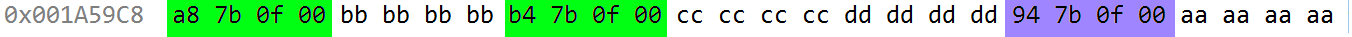
\includegraphics[width=\textwidth]{img/polymorfizmus2.png} \\
\vskip 1ex
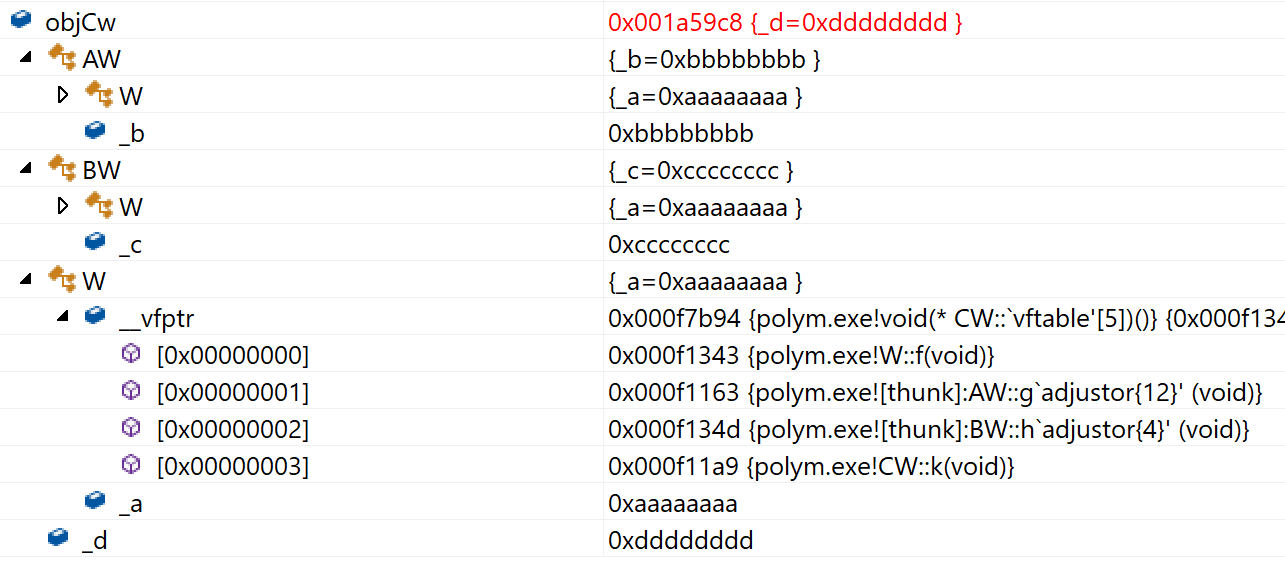
\includegraphics[width=\textwidth]{img/polymorfizmus.png}
\end{frame}

\zkouskove

% třídní ukazatele
% 04
%
\hkapitola{Výjimky}

\begin{frame}[fragile]

\begin{bitemize}{Výjimky}
\item slouží k ošetření chybových stavů v programu
\item systém je velmi podobný Javě
\item[]
\item vyvolání výjimky \lstinline|throw ...|
\item zachycení a zpracování výjimky \lstinline|try - catch - finally|
\item výjimky odvozeny od základní třídy \lstinline|System.Exception|
\item[]
\item nezachycená výjimka se šíří z metody dále
\begin{itemize}
\item na nejvyšší úrovni způsobí pád programu s chybovým hlášením
\end{itemize}

\end{bitemize}

\end{frame}




\begin{frame}[fragile]
\vfill
\begin{bitemize}{Vyvolání výjimky}
\item \lstinline|throw objektVýjimky|
\end{bitemize}
\vfill
\begin{yesblock}
\begin{lstlisting}
static void ComplexCalculation()
{
    throw new InvalidOperationException("broken toe");
}
\end{lstlisting}
\end{yesblock}
\vfill
\end{frame}



\begin{frame}[fragile]
\begin{bitemize}{Zachycení výjimky}
\item \lstinline|catch (typVýjimky názevProměnné)|
\end{bitemize}
\vfill
\begin{yesblock}
\begin{lstlisting}
try
{
    Console.WriteLine("pre throw");
    ComplexCalculation();
    Console.WriteLine("post throw");
}
catch (Exception ex)
{
    Console.Error.WriteLine(ex.Message);
}
\end{lstlisting}
\end{yesblock}
\end{frame}



\begin{frame}[fragile]
\begin{bitemize}{Zachycení výjimky -- univerzální catch}
\item \lstinline|catch|
\end{bitemize}
\vfill
\begin{yesblock}
\begin{lstlisting}
try
{
    Console.WriteLine("pre throw");
    ComplexCalculation();
    Console.WriteLine("post throw");
}
catch 
{
    Console.Error.WriteLine("catched something");
}
\end{lstlisting}
\end{yesblock}
\end{frame}


\begin{frame}[fragile]
\begin{bitemize}{Blok finally}
\item \lstinline|finally| -- nepovinné, blok je proveden vždy
\end{bitemize}
\vfill
\begin{yesblock}
\begin{lstlisting}
try
{
    Console.WriteLine("pre throw");
    ComplexCalculation();
    Console.WriteLine("post throw");
}
catch (Exception ex)
{
    Console.Error.WriteLine(ex.Message);
}
finally
{
    Console.WriteLine("finally");
}
\end{lstlisting}
\end{yesblock}
\end{frame}





\begin{frame}[fragile]
\frametitle{Třída System.Exception}
\begin{noteblock}{}
\begin{lstlisting}
public class Exception : ISerializable, _Exception
{
    public Exception();
    public Exception(string message);
    public Exception(string message, Exception innerException);

    public virtual string Source { get; set; }
    public virtual string HelpLink { get; set; }
    public virtual string StackTrace { get; }
    public MethodBase TargetSite { get; }
    public Exception InnerException { get; }
    public virtual string Message { get; }
    public int HResult { get; protected set; }
    public virtual IDictionary Data { get; }
    
    // ...
}
\end{lstlisting}
\end{noteblock}

\end{frame}



\begin{frame}[fragile]
\frametitle{Potomci třídy System.Exception}
\begin{noteblock}{}
\begin{itemize}
\item \lstinline|SystemException|
\item \lstinline|ApplicationException|
\item[]
\item \lstinline|IndexOutOfRangeException|
\item \lstinline|NullReferenceException|
\item \lstinline|AccessViolationException|
\item \lstinline|InvalidOperationException|
\item \lstinline|ArgumentException|
\item \lstinline|ArgumentNullException|
\item \lstinline|ArgumentOutOfRangeException|
\item \lstinline|ArithmeticException|
\item \lstinline|IndexOutOfRangeException|
\item \ldots
\end{itemize}
\end{noteblock}

\end{frame}




\begin{frame}[fragile]
\begin{bitemize}{Řízené použití prostředků pomocí try -- finally}
\item konstrukci \lstinline|try - finally| lze využít pro řízený přístup k prostředkům
\item blok \lstinline|finally| je proveden i v případě výskytu libovolné výjimky uvnitř \lstinline|try| bloku a je tak možné uklidit prostředky
\item rozhraní \lstinline|IDisposable| slouží k uvolnění těchto prostředků
\end{bitemize}
\vfill
\begin{yesblock}
\begin{lstlisting}
{
    Font font1 = new Font("Arial", 10.0f);
    try
    {
        byte charset = font1.GdiCharSet;
    }
    finally
    {
        if (font1 != null)
            ((IDisposable)font1).Dispose();
    }
}
\end{lstlisting}
\end{yesblock}
\end{frame}


\begin{frame}[fragile]
\vfill
\begin{bitemize}{Řízené použití prostředků pomocí try -- finally}
\item pro zjednodušení C\# nabízí ekvivalentní konstrukci \lstinline|using(...) { ... }|
\end{bitemize}
\vfill
\begin{yesblock} 
\begin{lstlisting}
using (Font font1 = new Font("Arial", 10.0f))
{
    byte charset = font1.GdiCharSet;
}
\end{lstlisting}
\end{yesblock}
\vfill
\begin{bitemize}{}
\item \lstinline|using| lze vnořovat nebo lze deklarovat více řízených proměnných najednou
\end{bitemize}
\vfill
\begin{yesblock}
\begin{lstlisting}
using (Font font3 = new Font("Arial", 10.0f),
            font4 = new Font("Arial", 10.0f))
{
    // Use font3 and font4.
}
\end{lstlisting}
\end{yesblock}
\end{frame}


\begin{frame}[fragile]
\begin{bitemize}{Kdy používat using}
\item nad objekty realizující rozhraní \lstinline|IDisposable|
\item \lstinline|System.IO, System.Net| -- třídy realizující operace se soubory/síťovými proudy
\item \lstinline|System.Data| -- třídy realizující databázové připojení a operace
\item \lstinline|System.Drawing| -- třídy popisující grafické objekty
\item \lstinline|System.Windows.Forms.Control| -- WinForms prvky
\item \ldots
\end{bitemize}
\end{frame}



%\hkapitola{Jmenné prostory}

\begin{frame}[fragile]
\frametitle{Jmenné prostory}

\begin{block}{}
\begin{itemize}
\item řeší konflikty jmen
\begin{itemize}
\item v C existuje jediný globální prostor
\item knihovní funkce se prefixují, aby nedošlo ke shodě (\lstinline|glutCreateWindow, png_image_begin_read_from_file|)
\end{itemize}

\item jmenné prostory jsou pouze balíkem funkcí, typů, proměnných, \ldots
\begin{itemize}
\item neřeší se zde viditelnost (neexistuje obdoba package-private)
\item lze vytvořit anonymní jmenný prostor pro ukrytí členů jen v rámci jednoho souboru
\end{itemize}

\item není definováno striktní fyzické uspořádání souborů
\begin{itemize}
\item Java -- balíček = složka, obsahuje pouze soubory v této složce
\item C++ -- jmenný prostor může být použit kdekoliv
\item C++ -- do existujícího jmenného prostoru je možno kdykoliv cokoliv přidat
\end{itemize}

\item jmenné prostory je možné vnořovat
\end{itemize}
\end{block}
\end{frame}



\begin{frame}[fragile]
\frametitle{Vytvoření jmenného prostoru}
\begin{noteblock}{}
\begin{lstlisting}
namespace názevJmennéhoProstoru {
  [deklarace/definice složek přidávaných <@do@> jm. prostoru] 
}
\end{lstlisting}
\end{noteblock}

\begin{block}{}
\begin{itemize}
\item jm. p. je možné vytvořit na globální úrovni nebo ve jmenném prostoru
\item jm. p. je možné opakovaně definovat -- vždy se přidají nové prvky do prostoru
\item přístup k prvkům jm. p. je pomocí operátoru \lstinline|::|
\end{itemize}
\end{block}
\end{frame}




\begin{frame}[fragile]
\frametitle{Přístup k prvkům jmenného prostoru z vnitřku}
\begin{yesblock}
\begin{lstlisting}
namespace System {

  void vymazKonzoli() { ... }

  void ukonciProgram() { 
    vymazKonzoli();
  }
}
\end{lstlisting}
\end{yesblock}
\end{frame}

\begin{frame}[fragile]
\frametitle{Přístup k prvkům jmenného prostoru zvenčí}
\begin{yesblock}
\begin{lstlisting}
namespace System {

  void vymazKonzoli() { ... }

  void ukonciProgram() { ... }
}
\end{lstlisting}
\end{yesblock}

\begin{yesblock}
\begin{lstlisting}
System::vymazKonzoli();
System::ukonciProgram();
\end{lstlisting}
\end{yesblock}
\end{frame}


\begin{frame}[fragile]
\frametitle{Přístup k prvkům jmenného prostoru zvenčí -- direktiva using}
\begin{yesblock}
\begin{lstlisting}
namespace System {

  void vymazKonzoli() { ... }

  void ukonciProgram() { ... }
}
\end{lstlisting}
\end{yesblock}

\begin{yesblock}
\begin{lstlisting}
using namespace System;

vymazKonzoli();
ukonciProgram();
\end{lstlisting}
\end{yesblock}
\end{frame}



\begin{frame}[fragile]
\frametitle{Přístup k prvkům jmenného prostoru zvenčí -- deklarace using}
\begin{yesblock}
\begin{lstlisting}
namespace System {

  void vymazKonzoli() { ... }

  void ukonciProgram() { ... }
}
\end{lstlisting}
\end{yesblock}

\begin{yesblock}
\begin{lstlisting}
using System::vymazKonzoli;

vymazKonzoli();
System::ukonciProgram(); // nelze "ukonciProgram()"!
\end{lstlisting}
\end{yesblock}
\end{frame}



\begin{frame}[fragile]
\begin{noblock}
\begin{itemize}
\item deklarace/direktiva \lstinline|using| by neměla být používána v hlavičkových souborech!!!
\begin{itemize}
\item každý, kdo provede \lstinline|#include| na daný soubor bude ovlivněn usingy
\begin{itemize}
\item pozor na řetězení závislostí (hrac.h $\rightarrow$ pohyblivy\_objekt.h $\rightarrow$ objekt.h)
\end{itemize}
\item může způsobit opět konflikty jmen
\end{itemize}
\end{itemize}
\end{noblock}
\end{frame}



\begin{frame}[fragile]
\frametitle{Otevřenost jmenných prostorů}
\begin{block}{}
\begin{itemize}
\item do jmenného prostoru jde vždy přidávat nové složky
\end{itemize}
\end{block}

\begin{yesblock}
\begin{lstlisting}[basicstyle=\small]
namespace Objekty {
  Kocka micka;
}

// ...

namespace Objekty {
  Kocka mourek;
}

Objekty::micka.mnoukni();
Objekty::mourek.mnoukni();
\end{lstlisting}
\end{yesblock}
\end{frame}


\begin{frame}[fragile]
\frametitle{Vnořování jmenných prostorů}
\begin{block}{}
\begin{itemize}
\item jmenné prostory lze libovolně vnořovat
\end{itemize}
\end{block}

\begin{yesblock}
\begin{lstlisting}
namespace Hra {
  namespace Objekty {
    namespace ZiveObjekty {
      struct NPC { ... };
    }
  }
}
\end{lstlisting}
\end{yesblock}

\begin{yesblock}
\begin{lstlisting}
Hra::Objekty::ZiveObjekty::NPC obchodnik{};
\end{lstlisting}
\end{yesblock}
\end{frame}




\begin{frame}[fragile]
\frametitle{Vnořování jmenných prostorů\ldots}
\begin{block}{}
\begin{itemize}
\item od C++17 podpora pro zkrácený zápis vnořených jm. p.
\end{itemize}
\end{block}

\begin{yesblock}
\begin{lstlisting}
namespace Hra::Objekty::ZiveObjekty {
  struct NPC { ... };
}
\end{lstlisting}
\end{yesblock}

\begin{yesblock}
\begin{lstlisting}
Hra::Objekty::ZiveObjekty::NPC obchodnik{};
\end{lstlisting}
\end{yesblock}
\end{frame}



\begin{frame}[fragile]
\begin{bonusblock}{Anonymní jmenné prostory}
\begin{itemize}
\item lze použít pro skrytí jeho složek jen pro daný soubor .cpp
\end{itemize}
\end{bonusblock}

\begin{bonusblock}{}
\begin{lstlisting}
namespace {
  int _anonymous = 123;
}

// dále ve stejném souboru
cout << _anonymous;
\end{lstlisting}
\end{bonusblock}
\end{frame}




% 05
%\hkapitola{Šablony}
\kapitola{Generické programování}

\begin{frame}[fragile]
\begin{twocols}
\begin{lstlisting}[basicstyle=\small]
void Vypis(int hodnota) {
  cout << hodnota << endl;
}
\end{lstlisting}
\vskip 1cm
\pause
\begin{lstlisting}[basicstyle=\small]
void Vypis(std::string hodnota) {
  cout << hodnota << endl;
}
\end{lstlisting}
\vskip 1cm
\pause
\begin{lstlisting}[basicstyle=\small]
void Vypis(Kocka& hodnota) {
  cout << hodnota << endl;
}
\end{lstlisting}

\twocolssep
\pause
\begin{lstlisting}[basicstyle=\small]
struct PoleIntu {
  int* _pole;
};
\end{lstlisting}
\vskip 1cm
\pause
\begin{lstlisting}[basicstyle=\small]
struct PoleStringu {
  std::string* _pole;
};
\end{lstlisting}
\vskip 1cm
\pause
\begin{lstlisting}[basicstyle=\small]
struct PoleKocek {
  Kocka* _pole;
};
\end{lstlisting}

\end{twocols}
\end{frame}






\begin{frame}[fragile]
\begin{twocols}
\begin{lstlisting}[basicstyle=\small]
void Vypis(int hodnota) {
  cout << hodnota << endl;
}
void Vypis(std::string hodnota) {
  cout << hodnota << endl;
}
void Vypis(Kocka& hodnota) {
  cout << hodnota << endl;
}
void Vypis(double hodnota) {
  cout << hodnota << endl;
}
void Vypis(bool hodnota) {
  cout << hodnota << endl;
}
void Vypis(Pes& hodnota) {
  cout << hodnota << endl;
}
void Vypis(Kralik& hodnota) {
  cout << hodnota << endl;
}
\end{lstlisting}

\twocolssep

\begin{lstlisting}[basicstyle=\small]
struct PoleIntu {
  int* _pole;
};
struct PoleStringu {
  std::string* _pole;
};
struct PoleKocek {
  Kocka* _pole;
};
struct PoleDoublu {
  double* _pole;
};
struct PoleBoolu {
  bool* _pole;
};
struct PolePsu {
  Pes* _pole;
};
struct PoleKraliku {
  Kralik* _pole;
};
\end{lstlisting}

\end{twocols}
\end{frame}












\begin{frame}[fragile]
\begin{twocols}
\begin{lstlisting}[basicstyle=\scriptsize]
void Vypis(int hodnota) {
  cout << hodnota << endl;
}
void Vypis(std::string hodnota) {
  cout << hodnota << endl;
}
void Vypis(Kocka& hodnota) {
  cout << hodnota << endl;
}
void Vypis(double hodnota) {
  cout << hodnota << endl;
}
void Vypis(bool hodnota) {
  cout << hodnota << endl;
}
void Vypis(Pes& hodnota) {
  cout << hodnota << endl;
}
void Vypis(Kralik& hodnota) {
  cout << hodnota << endl;
}
void Vypis(unsigned int hodnota) {
  cout << hodnota << endl;
}
void Vypis(long long hodnota) {
  cout << hodnota << endl;
}
void Vypis(exception& hodnota) {
  cout << hodnota << endl;
}
\end{lstlisting}

\twocolssep

\begin{lstlisting}[basicstyle=\scriptsize]
struct PoleIntu {
  int* _pole;
};
struct PoleStringu {
  std::string* _pole;
};
struct PoleKocek {
  Kocka* _pole;
};
struct PoleDoublu {
  double* _pole;
};
struct PoleBoolu {
  bool* _pole;
};
struct PolePsu {
  Pes* _pole;
};
struct PoleKraliku {
  Kralik* _pole;
};
struct PoleUIntu {
  unsigned int* _pole;
};
struct PoleLongLong {
  long long* _pole;
};
struct PoleException {
  exception* _pole;
};
\end{lstlisting}

\end{twocols}
\end{frame}












\begin{frame}[fragile]
\begin{block}{Generické programování}
\begin{itemize}
\item využívá abstraktních vzorů funkcí a tříd
\item základem jsou šablony (templates)
\end{itemize}
\end{block}

\begin{block}{Šablony}
\begin{itemize}
\item podobné makrům preprocesoru
\item zpracovává je kompilátor
\item umožňují pracovat s parametry, které jsou obecného datového typu
\item jedna šablona může definovat celou množinu funkcí/tříd
\end{itemize}
\end{block}
\end{frame}



\begin{frame}[fragile]
\begin{yesblock}
\begin{lstlisting}
template<typename T>
void Vypis(T& hodnota) {
  cout << hodnota << endl;
}

template<typename T>
struct Pole {
  T* _pole;
};
\end{lstlisting}
\end{yesblock}
\end{frame}








\begin{frame}[fragile]
\begin{block}{Šablona třídy?}
\begin{itemize}
\item šablona
\begin{itemize}
\item to co programátor vytvoří
\item kus zdrojového kódu, který se vlastně ani použít nemusí
\end{itemize}
\vskip 2ex
\item instance šablony
\begin{itemize}
\item konkrétní datový typ
\item vytvoří kompilátor (automaticky/na vyžádání)
\item kus binárního kódu, který se pak používá
\end{itemize}
\vskip 2ex
\item objekt
\begin{itemize}
\item typu \uv{instance šablony}
\end{itemize}
\end{itemize}
\end{block}
\end{frame}










\begin{frame}[fragile]
\begin{twocols}
\begin{center}
\color{blue} \bfseries
Programátor
\end{center}

\twocolssep

\begin{center}
\color{red} \bfseries
Kompilátor
\end{center}
\end{twocols}
\pause
\begin{center}
\bfseries Šablona 
\end{center}

\begin{center}
\begin{minipage}{5cm}
\vskip -2ex
\begin{exampleblock}{}
\begin{lstlisting}[basicstyle=\scriptsize]
template<typename T>
struct Pole {
  T* _pole;
};
\end{lstlisting}
\end{exampleblock}

\end{minipage}
\end{center}
\pause
\begin{center}
\bfseries Instance šablony 
\end{center}
\vskip -2ex

\begin{twocols}

\begin{exampleblock}{}
\begin{lstlisting}[basicstyle=\scriptsize]
// vytvořena automaticky na pozadí
\end{lstlisting}
\end{exampleblock}

\twocolssep

\begin{noteblock}{}
\begin{lstlisting}[basicstyle=\scriptsize]
struct .?AU?<@\$@>Pole@H@@ {
  int* _pole;
};
\end{lstlisting}
\end{noteblock}
\end{twocols}

\pause
\begin{center}
\bfseries Objekt 
\end{center}
\vskip -2ex

\begin{twocols}
\begin{exampleblock}{}
\begin{lstlisting}[basicstyle=\scriptsize]
Pole<int> poleIntu{};
\end{lstlisting}
\end{exampleblock}

\twocolssep

\begin{noteblock}{}
\begin{lstlisting}[basicstyle=\scriptsize]
.?AU?<@\$@>Pole@H@@ poleIntu{};
\end{lstlisting}
\end{noteblock}
\end{twocols}
\end{frame}










\kapitola{Šablona a její parametry}



\begin{frame}[fragile]
\frametitle{Šablona}
\begin{block}{}
\begin{itemize}
\item je generický předpis funkce, typu nebo metody
\item definuje seznam parametrů šablony (typové, hodnotové)
\begin{itemize}
\item uvnitř šablony jsou to konstanty
\end{itemize}

\item pro jednu funkci, typ nebo metodu může existovat více variant šablon
\begin{itemize}
\item základní šablona
\item explicitní specializace šablony
\item parciální specializace šablony (pouze šablony typů)
\end{itemize}
\end{itemize}
\end{block}

\end{frame}




\begin{frame}[fragile]
\frametitle{Šablona}
\begin{noteblock}{}
\begin{lstlisting}
template<parametrŠablony... , ...>
deklaraceNeboDefiniceFunkceTypuMetody;

parametrŠablony:
  typename|class názevParametru
  typHodnotovéhoTypu názevParametru
  template<...> typename názevParametru
\end{lstlisting}
\end{noteblock}

\begin{block}{Parametry šablony}
\begin{itemize}
\item uvnitř instance šablony představují \textbf{konstantní hodnoty}
\item mohou představovat typ, konkrétní hodnotu (číslo, ukazatel, \ldots) nebo vnořenou šablonu
\end{itemize}
\end{block}
\end{frame}




\begin{frame}[fragile]
\frametitle{Typové parametry}
\begin{block}{}
\begin{itemize}
\item představují libovolný datový typ (primitivní i objektový)
\item jakmile je zvolen je uvnitř šablony uplatňována standardní striktní typová kontrola
\item používá se zástupné slovo \lstinline|typename| nebo \lstinline|class| (starší, stále dostupné z důvodu zpětné kompatibility)
\end{itemize}
\end{block}

\begin{yesblock}
\begin{lstlisting}
template<typename ParametrSablony> 
struct Pole {
  ParametrSablony _array[10];
};

Pole<int> poleIntu{};
Pole<Kocka> poleKocek{};
\end{lstlisting}
\end{yesblock}
\end{frame}





\begin{frame}[fragile]
\frametitle{Hodnotové parametry}
\vskip -1ex
\begin{block}{}
\begin{itemize}
\item představují konkrétní (číselnou) hodnotu
\begin{itemize}
\item celočíselný parametr
\item výčtový 
\item ukazatel na objekt
\item reference na objekt
\item ukazatel na funkci
\item třídní ukazatel
\end{itemize}

\item uvnitř šablony představují neměnné konstanty
\end{itemize}
\end{block}

\vskip -1ex
\begin{yesblock}
\begin{lstlisting}[basicstyle=\small]
template<int CiselnyParametr> 
struct Pole {
  int _array[CiselnyParametr];
};

Pole<10> poleDesetiIntu{};
Pole<50> polePadesatiIntu{};
\end{lstlisting}
\end{yesblock}
\end{frame}




\begin{frame}[fragile]
\frametitle{Hodnotové parametry\ldots}
\begin{yesblock}
\begin{lstlisting}[basicstyle=\scriptsize]
enum TypObjektu { Kamen, Strom, Ker, Trava };

template<TypObjektu typ> 
struct Pole {
  void* _array[10];
};

Pole<Kamen> poleSutru{};
Pole<Strom> poleStromecku{};
\end{lstlisting}
\end{yesblock}

\begin{yesblock}
\begin{lstlisting}[basicstyle=\scriptsize]
void func1(Object* ptr) { ... }
void func2(Object* ptr) { ... }

template<void (*function) (Object*)> 
struct Pole {
  void* _array[10];
};

Pole<func1> poleSFunkci1{};
Pole<func2> poleSFunkci2{};
\end{lstlisting}
\end{yesblock}
\end{frame}






\begin{frame}[fragile]
\frametitle{Parametrů může být více}
\begin{yesblock}
\begin{lstlisting}[basicstyle=\small]
template<typename Typ, int VelikostPole> 
struct Pole {
  Typ _array[VelikostPole];
};

Pole<Kamen, 10> poleDesetiSutru{};
Pole<Strom, 3> poleTriStromecku{};
\end{lstlisting}
\end{yesblock}

\begin{bonusblock}{Variadic templates\cpp{11}}
\begin{itemize}
\item C++11 zavedlo šablony s proměnným počtem parametrů
\item \lstinline|template<typename... args> struct StructWithVarArgs { };|
\item část parametrů může být specifikována konkrétně
\begin{itemize}
\item \lstinline|template<typename First, typename... Rest> struct...|
\end{itemize}
\end{itemize}
\end{bonusblock}
\end{frame}







\begin{frame}[fragile]
\frametitle{Instance šablony}

\begin{block}{}
\begin{itemize}
\item instance šablony představuje konkrétní datový typ nebo kód funkce, který překladač vytvoří po dosazení parametrů šablony
\item kompilátor ji vytváří automaticky (při použití typu/funkce)
\begin{itemize}
\item lze také vynutit explicitní vytvoření
\end{itemize}
\item []
\item \textbf{pokud chcete, aby kompilátor zkontroloval \uv{obsah} šablony, je potřeba instance šablony a její použití!}
\item \textbf{aby mohla vzniknout instance šablony, je nutné znát kompletní definici šablonové funkce/typu (proto se šablony celé píšou do hlavičkových souborů)}

\end{itemize}
\end{block}
\end{frame}


\begin{frame}[fragile]
\frametitle{Instance šablony\ldots}
\begin{yesblock}
\begin{lstlisting}
template<typename T> 
struct Pole { 
  ... 
};
\end{lstlisting}
\end{yesblock}

\begin{yesblock}
\begin{lstlisting}
// explicitní vytvoření instance šablony Pole<int>
template struct Pole<int>; 

// implicitní vytvoření instance šablony Pole<string>
Pole<string> globalniPoleStringu{};
\end{lstlisting}
\end{yesblock}
\end{frame}



\kapitola{Použití šablon}
\pkapitola{Šablony funkcí}

\begin{frame}[fragile]
\begin{block}{}
\begin{itemize}
\item funkce podporují automatické odvození parametrů šablony
\begin{itemize}
\item parametry musí vhodně odpovídat, nesmí dojít ke sporné situace
\end{itemize}
\end{itemize}
\end{block}
	
\begin{yesblock}
\begin{lstlisting}
template<typename Typ>
void vypis(const Typ& vystup) {
  cout << vystup;
}
\end{lstlisting}
\end{yesblock}

\begin{yesblock}
\begin{lstlisting}
int intyzr = 123;
double dabl = 3.141592;

vypis<int>(intyzr); // explicitní uvedení parametrů šablony
vypis(dabl); // kompilátor automaticky odvodí parametry šablony
\end{lstlisting}
\end{yesblock}
\end{frame}



\begin{frame}[fragile]
\begin{yesblock}
\begin{lstlisting}
template<typename Typ>
bool porovnej(const Typ& a, const Typ& b) {
  return a == b;
}
\end{lstlisting}
\end{yesblock}

\begin{yesblock}
\begin{lstlisting}
int intyzrAlfa = 123;
int intyzrBeta = 456;
double dabl = 3.141592;

bool vysledek;
vysledek = porovnej(intyzrAlfa, intyzrBeta);
\end{lstlisting}
\end{yesblock}
\vskip -4ex
\begin{noblock}
\begin{lstlisting}
vysledek = porovnej(intyzrAlfa, dabl); // int,double?!?
\end{lstlisting}
\end{noblock}
\end{frame}



\pkapitola{Šablony objektových typů}



\begin{frame}[fragile]
\begin{block}{}
\begin{itemize}
\item u struktur a tříd je nutné vždy definovat parametry šablony
\begin{itemize}
\item při splnění určitých podmínek je automatické odvození parametrů podporováno od C++17
\end{itemize}
\end{itemize}
\end{block}

\begin{yesblock}
\begin{lstlisting}
template<typename Typ>
struct Pole {
  ...
};
\end{lstlisting}
\end{yesblock}

\begin{yesblock}
\begin{lstlisting}
Pole<int> poleIntu{};
Pole<string> poleStringu{};
\end{lstlisting}
\end{yesblock}

\end{frame}








\begin{frame}[fragile]
\begin{block}{}
\begin{itemize}
\item složky definované uvnitř typu zapisujeme bez úprav
\end{itemize}
\end{block}

\begin{yesblock}
\begin{lstlisting}
template<typename Typ>
struct Pole {
  
  const Typ& dej(int index) const {
    return _pole[index];
  }

private:
  Typ _pole[10];
};
\end{lstlisting}
\end{yesblock}

\end{frame}







\begin{frame}[fragile]
\vskip -1.5ex
\begin{block}{}
\begin{itemize}
\item složky definované vně typu musí oznámit kompilátoru, že se jedná o šablonu
\begin{itemize}
\item je nutné definovat s jakými parametry pracujeme
\end{itemize}
\end{itemize}
\end{block}
\vskip -1.5ex
\begin{yesblock}
\begin{lstlisting}[basicstyle=\small]
template<typename Typ>
struct Pole {
 
  const Typ& dej(int index) const;

private:
  Typ _pole[10];
};

template<typename Typ> // <@$\commentcolor\leftarrow$@> je to šablona a jaké má parametry
//==============
const Typ& Pole<Typ>::dej(int index) const {
// <@\hskip 1.9cm@> ===== <@$\commentcolor\leftarrow$@> jaká konkrétní varianta šablony to je
  return _pole[index];
}
\end{lstlisting}
\end{yesblock}
\end{frame}






\begin{frame}[fragile]
\begin{block}{}
\begin{itemize}
\item statické atributy se definují jako šablony
\end{itemize}
\end{block}

\begin{yesblock}
\begin{lstlisting}
template <typename T>
struct Pole {

  static int PocetPoli;

};

template <typename T>
int Pole<T>::PocetPoli = 0;
\end{lstlisting}
\end{yesblock}
\end{frame}




\kapitola{Vnořené šablony}



\begin{frame}[fragile]
\begin{block}{}
\begin{itemize}
\item představuje šablonu v šabloně
\item ve vnořených šablonách je možné pracovat s
\begin{itemize}
\item aktuálními šablonovými parametry
\item i s parametry nadřazených šablon
\end{itemize}

\item při vytvoření instance nadřazené šablony nevznikají automaticky instance vnořených šablon
\end{itemize}
\end{block}
\end{frame}


\begin{frame}[fragile]
\begin{block}{}
\begin{itemize}
\item uvnitř šablony je možné definovat další šablony (vnořené typy, metody)
\end{itemize}
\end{block}

\begin{yesblock}
\begin{lstlisting}[basicstyle=\small]
template <typename T>
struct Pole {
  
  template <typename U>
  U collect(U (*funkce)(U, T*), U init) {
    U tmp = init;
    for (auto&& item : _pole)      
      tmp = funkce(tmp, &item);

    return tmp;
  }

private:
  T _pole[10];
};
\end{lstlisting}
\end{yesblock}
\end{frame}


\begin{frame}[fragile]
\begin{block}{}
\begin{itemize}
\item vnější definice vnořené šablony vyžaduje definování všech šablon
\end{itemize}
\end{block}
\vskip -1ex
\begin{yesblock}
\begin{lstlisting}[basicstyle=\small]
template <typename T>
struct Pole {
  
  template <typename U>
  U collect(U (*funkce)(U, T*), U init);
};

template <typename T>
template <typename U>
U Pole<T>::collect(U (*funkce)(U, T*), U init) {
  U tmp = init;
  for (auto&& item : _pole)      
    tmp = funkce(tmp, &item);

  return tmp;
}
\end{lstlisting}
\end{yesblock}
\end{frame}







\kapitola{Závislá jména}


\begin{frame}[fragile]
\begin{block}{}
\begin{itemize}
\item pokud pracujeme s obecným typem a ten představuje komplexní typ může se objevit problém závislých jmen
\item nelze přímo pracovat s vnořenými typy pod obecným typem (nebo závislých na obecném typu)
\begin{itemize}
\item kompilátor je nevidí
\end{itemize}
\item nelze přímo pracovat s vnořenými šablonami pod obecným typem (nebo závislých na obecném typu)
\begin{itemize}
\item kompilátor je nevidí
\end{itemize}
\end{itemize}
\end{block}


\begin{noblock}
\begin{lstlisting}
template<typename T>
struct S {
  T::iterator _iter; // <@\commentcolor$\leftarrow$@> error - neznám "T::iterator"
};
\end{lstlisting}
\end{noblock}
\end{frame}
















\begin{frame}[fragile]
\begin{block}{}
\begin{itemize}
\item vnořený typ je nutné označit pomocí \lstinline|typename|
\end{itemize}
\end{block}


\begin{noblock}
\begin{lstlisting}
template<typename T>
struct S {
  T::iterator _iter; // <@\commentcolor$\leftarrow$@> error - neznám "T::iterator"
};
\end{lstlisting}
\end{noblock}

\begin{yesblock}
\begin{lstlisting}
template<typename T>
struct S {
  typename T::iterator _iter;
};
\end{lstlisting}
\end{yesblock}
\end{frame}











\begin{frame}[fragile]
\begin{block}{}
\begin{itemize}
\item \lstinline|typedef| rovněž musí použít \lstinline|typename|
\end{itemize}
\end{block}

\begin{noblock}
\begin{lstlisting}
template<typename T>
struct S {
  typedef T::iterator TIterator; // <@\commentcolor$\leftarrow$@> error - neznám "T::iterator"
  TIterator _iter;
};
\end{lstlisting}
\end{noblock}

\begin{yesblock}
\begin{lstlisting}
template<typename T>
struct S {
  typedef typename T::iterator TIterator;
  TIterator _iter;
};
\end{lstlisting}
\end{yesblock}
\end{frame}










\begin{frame}[fragile]
\begin{block}{}
\begin{itemize}
\item pro použití vnořených šablon je potřeba \lstinline|template|
\end{itemize}
\end{block}

\begin{noblock}
\begin{lstlisting}[basicstyle=\small]
struct Usage {
  template<typename U>
  void method() {
    ...
  }
};

// předpokládejme T = Usage
template<typename T>
struct Template {
  void m() {
    T t{};
    t.method<int>(); // <@\commentcolor$\leftarrow$@> error - neznám "t.method"
  }
};
\end{lstlisting}
\end{noblock}
\end{frame}






\begin{frame}[fragile]
\begin{block}{}
\begin{itemize}
\item pro použití vnořených šablon je potřeba \lstinline|template|
\end{itemize}
\end{block}

\begin{yesblock}
\begin{lstlisting}[basicstyle=\small]
struct Usage {
  template<typename U>
  void method() {
    ...
  }
};

// předpokládejme T = Usage
template<typename T>
struct Template {
  void m() {
    T t{};
    t.template method<int>();
  }
};
\end{lstlisting}
\end{yesblock}
\end{frame}









\begin{frame}[fragile]
\begin{block}{}
\begin{itemize}
\item oba uvedené případy se mohou i kombinovat\ldots
\end{itemize}
\end{block}
\end{frame}


\begin{frame}[fragile]
\begin{yesblock}
\begin{lstlisting}[basicstyle=\scriptsize]
struct Usage {
    template<typename TT>
    struct NestedTemplateStruct {
        struct iterator {
            int _x = 123;
        };
    };
};


// předpokládejme T = Usage
template<typename T>
struct Template {
	
    void m() {
        T t{};
        typename T::template NestedTemplateStruct<int>::iterator iteratorVar;
        cout << iteratorVar._x << endl;
    }
};
\end{lstlisting}
\end{yesblock}
\end{frame}



\nezkouskove

\kapitola{Specializace šablon}
\pkapitola{Explicitní specializace}

\begin{frame}[fragile]
\frametitle{Explicitní specializace}
\begin{block}{}
\begin{itemize}
\item představuje jinou realizaci šablony (vlastní kód je nově definovaný) pro konkrétní sadu parametrů
\begin{itemize}
\item s původní šablonou sdílí jenom jméno (kód ne!)
\end{itemize}
\item použitelné pro šablony funkcí i typů
\item může existovat mnoho explicitních specializací jedné šablony
\end{itemize}
\end{block}

\begin{noteblock}{}
\begin{itemize}
\item definuje se po definici základní šablony
\item definuje se jako šablona, ale
\begin{itemize}
\item nemá obecné šablonové parametry (uvádí se \lstinline|template<>|)
\item za názvem typu/funkce se uvádí konkrétní sada parametrů, pro kterou tato šablona bude použita (\lstinline|... sablonaFunkce<int>() ...|)
\end{itemize}
\end{itemize}
\end{noteblock}
\end{frame}





\begin{frame}[fragile]
\frametitle{Explicitní specializace funkce}
\begin{yesblock}
\begin{lstlisting}[basicstyle=\small]
// Základní šablona
template<typename T>
void printTemplate(string name, T value) {
	cout << name << ": " << value << endl;
}

// Explicitní specializace
template<> 
// explicitní specializace je šablonou, ale všechny parametry jsou konkrétní hodnoty
void printTemplate<double>(string name, double value) {
	cout << name << ": " << fixed << setprecision(3) << value << endl;
}

printTemplate("Char", 'x'); // Char: 'x'
printTemplate("Int", 15);  // Int: 15
printTemplate("Double", 3.14); // Double: 3.140
\end{lstlisting}
\end{yesblock}
\end{frame}




\begin{frame}[fragile]
\frametitle{Explicitní specializace třídy}
\begin{yesblock}
\begin{lstlisting}[basicstyle=\small]
// Základní šablona
template<typename T>
struct Comparator : ComparatorBase {

  int compare(const T& a, const T& b) const;
};

template<typename T>
int Comparator<T>::compare(const T& a, const T& b) const {
  return b - a;
}
\end{lstlisting}
\end{yesblock}
\end{frame}


\begin{frame}[fragile]
\frametitle{Explicitní specializace třídy\ldots}
\begin{yesblock}
\begin{lstlisting}[basicstyle=\small]
// Explicitní specializace
template<>
struct Comparator<const char*> : ComparatorBase {

  int compare(const char* a, const char* b) const;
};

// metody explicitně specializované třídy se definují bez template<>
int Comparator<const char*>::compare(const char* a, const char* b) const {
  return strcmp(a, b);
}	
\end{lstlisting}
\end{yesblock}
\end{frame}


\begin{frame}[fragile]
\frametitle{Explicitní specializace třídy\ldots}
\begin{yesblock}
\begin{lstlisting}[basicstyle=\small]
struct ComparatorBase {
  constexpr static int FIRST_IS_BIGGER = 1;
  constexpr static int EQUAL = 0;
  constexpr static int SECOND_IS_BIGGER = -1;
};
\end{lstlisting}
\end{yesblock}

\begin{yesblock}
\begin{lstlisting}[basicstyle=\small]
Comparator<int> cInt{};
cout << (cInt.compare(20, 40) == Comparator<int>::FIRST_IS_BIGGER ? "20 > 40" : "20 <= 40") << endl;

Comparator<const char*> cCstr{};
int result = cCstr.compare("hello", "hella");
\end{lstlisting}
\end{yesblock}
\end{frame}















\pkapitola{Parciální specializace}

\begin{frame}[fragile]
\frametitle{Parciální specializace}
\begin{block}{}
\begin{itemize}
\item představuje jinou realizaci šablony (vlastní kód je nově definovaný) pro částečně specifikované parametry šablony
\begin{itemize}
\item s původní šablonou sdílí jenom jméno (kód ne!)
\end{itemize}
\item použitelné pouze pro šablony typů
\item může existovat mnoho parciálních specializací jedné šablony
\end{itemize}
\end{block}

\begin{noteblock}{}
\begin{itemize}
\item definuje se po definici základní šablony
\item definuje se jako šablona, ale
\begin{itemize}
\item má obecné/konkrétní/částečně specifikované šablonové parametry (uvádí se \lstinline|template<...>|)
\item za názvem typu/funkce se uvádí konkrétní sada parametrů, pro kterou tato šablona bude použita (\lstinline|... SablonaTridy<int, T>() ...|)
\end{itemize}
\end{itemize}
\end{noteblock}
\end{frame}



\begin{frame}[fragile]
\frametitle{Co a jak lze specializovat - parciálně?}
\begin{yesblock}
\begin{lstlisting}[basicstyle=\small]
template<typename T, typename U, int S>
struct Template { }; 

// lze některé parametry přesně definovat (jako u explicitní specializace)
// zde definujeme S
template<typename T, typename U>
struct Template<T, U, 10> { }; 

// zde definujeme U a S
template<typename T>
struct Template<T, int, 10> { }; 

// lze některé typové parametry označit za obecné ukazatele
// zde definujeme T jako libovolný ukazatel
template<typename T, typename U, int S>
struct Template<T*, U, S> { }; 
\end{lstlisting}
\end{yesblock}
\end{frame}




\begin{frame}[fragile]
%\frametitle{}
\begin{block}{Jedna věc může být definována jako}
\begin{itemize}
\item základní šablona
\item několik parciálních specializací
\item několik explicitních specializací
\end{itemize}
\end{block}

\begin{block}{}
\begin{itemize}
\item kompilátor pak vybírá nejvhodnější sadu parametrů
\begin{itemize}
\item přesná shoda s explicitní specializací
\item shoda s parciální specializací
\item jako nouzovka -- základní šablona
\end{itemize}
\item nesmí dojít ke shodě u více parciálních specializací
\begin{itemize}
\item \lstinline|<T*, U>| a \lstinline|<T, U*>| -- co použít pro \lstinline|<int*, int*>|
\end{itemize}
\end{itemize}
\end{block}
\end{frame}




\begin{frame}[fragile]
\frametitle{Parciální specializace\ldots}
\begin{yesblock}
\begin{lstlisting}
template<typename T>
struct Comparator<T*> : ComparatorBase {

  int compare(T* a, T* b) const;
};

template<typename T>
int Comparator<T*>::compare(T* a, T* b) const {
  return *b - *a;
}
\end{lstlisting}
\end{yesblock}
\end{frame}

\begin{frame}[fragile]
\frametitle{Parciální specializace\ldots}
\begin{yesblock}
\begin{lstlisting}
Comparator<int*> cInt{};

int* a = new int{ 20 };
int* b = new int{ 40 };

cout << (cInt.compare(a, b) == Comparator<int>::FIRST_IS_BIGGER ? "20 > 40" : "20 <= 40") << endl;
\end{lstlisting}
\end{yesblock}
\end{frame}

\zkouskove

% 06
%\hkapitola{Datové proudy}

\begin{frame}[fragile]
\frametitle{string}

\begin{block}{<string>}
\begin{itemize}
\item třída string je realizována šablonou \lstinline|basic_string<char>|
\item rozhraní zapadá do konceptu STL kontejnerů (viz později), chová se jako kontejner znaků
\item umožňuje jednodušše upravovat, vyhledávat, procházet řetězec
\end{itemize}
\end{block}

\begin{yesblock}
\begin{lstlisting}
string s1 = "hello world";
string s2{ "hello world" };
string s3 = s2;
string s4 = s1 + s2;

cout << s4.c_str() << endl;
\end{lstlisting}
\end{yesblock}
\end{frame}


\begin{frame}[fragile]
\frametitle{string -- základní metody a vlastnosti}

\begin{block}{}
\begin{itemize}
\item \lstinline|operator[]| -- procházení znaků
\item \lstinline|c_str()| -- konverze na \lstinline|const char*|
\item \lstinline|begin(), end()| -- iterátory
\item \lstinline|empty(), size()| -- test prázdnosti/test délky řetězce
\item \lstinline|insert(), erase()| -- vkládání, mazání znaků
\item \lstinline|substr()| -- výběr podřetězce
\item \lstinline|find(), rfind()| -- hledání podřetězce
\item \lstinline|find_first_of(), find_first_not_of()| -- hledání znaků
\item \lstinline|find_last_of(), find_last_not_of()| -- hledání znaků
\item porovávací operátory, \lstinline|replace()|, \lstinline|at()|, \lstinline|data()|, \ldots
\end{itemize}
\end{block}
\end{frame}


\begin{frame}[fragile]
\frametitle{Datové proudy}

\begin{block}{}
\begin{itemize}
\item nízkoúrovňové datové proudy zabaleny do objektů s jednoduchým rozhraním
\item proudy pro práci s konzolí, soubory a paměťový proud
\item jedná se o součást STL, ale neposkytují iterátorové rozhraní
\begin{itemize}
\item v knihovně jsou k dispozici adaptéry pro napojení na iterátory
\end{itemize}
\item vstup a výstup dat pomocí metod a přetížených operátorů (\lstinline|<<, >>|)
\end{itemize}
\end{block}


\begin{block}{}
\centering
\begin{tabular}{cccc}
\bfseries objekt & \bfseries instance třídy & \bfseries popis & \bfseries lowlevel proud (C) \\
\lstinline|cout| & \lstinline|ostream| & výstupní proud  & \lstinline|stdout| \\
\lstinline|cin| & \lstinline|istream| & vstupní proud & \lstinline|stdin| \\
\lstinline|cerr| & \lstinline|ostream| & chybový výstup & \lstinline|stderr| \\
\end{tabular}
\end{block}
\end{frame}





\begin{frame}[fragile]
\begin{yesblock}
\begin{lstlisting}
#include <iostream>
using namespace std;

int main(void)
{ 
	int cislo; 

	// výpis textu na obrazovku s odřádkováním
	cout << "Napis cislo" << endl; 
	// načtení celého čísla z klávesnice
	cin >> cislo; 

	cout << "Napsal jsi: " << cislo << endl; 
	return 0; 
}
\end{lstlisting}
\end{yesblock}
\end{frame}




\begin{frame}[fragile]
\frametitle{Manipulátory}
\begin{block}{}
\begin{itemize}
\item formát výstupu lze jednoduše přizpůsobit pomocí manipulátorů
\begin{itemize}
\item jednoduché objekty, které přenastaví proud
\end{itemize}
\item knihovna obsahuje řadu připravených manipulátorů
\begin{itemize}
\item lze definovat vlastní manipulátory
\end{itemize}
\item hlavičkový soubor \lstinline|<iomanip>|
\end{itemize}
\end{block}

\begin{yesblock}
\begin{lstlisting}
int val = 15;
cout << val << " 0x" << hex << val << endl;
// vypíše: 15 0xf
\end{lstlisting}
\end{yesblock}
\end{frame}






\begin{frame}[fragile]
\frametitle{Knihovní manipulátory}

\begin{block}{}
\begin{itemize}
\item \lstinline|endl| -- konec řádku a vyprázdnění bufferu
\item \lstinline|flush| -- vyprázdnění bufferu
\item \lstinline|dec, hex, oct| -- výpis čísel v desítkové, šestnáctkové nebo osmičkové soustavě
\item \lstinline|setbase(int)| -- výpis čísel v zadané soustavě
\item \lstinline|setw(int)| -- nastaví šířku vypisované hodnoty (na kolik znaků zarovnávat)
\item \lstinline|setfill(char)| -- nastaví vyplňovací znak
\item \lstinline|setprecision(int)| -- nastaví vypisovanou přesnost reálných čísel
\end{itemize}
\end{block}

\begin{yesblock}
\begin{lstlisting}[basicstyle=\small]
int c = 7;
cout << setw(3) << c << endl;
cout << setw(4) << setfill('@') << hex << c << endl;
\end{lstlisting}
\end{yesblock}
\end{frame}








\begin{frame}[fragile]
\frametitle{Hierarchie tříd proudů}

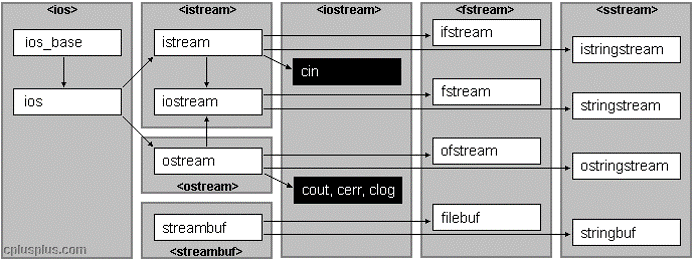
\includegraphics[width=\textwidth]{img/streamy.png}
\end{frame}






\begin{frame}[fragile]
\frametitle{Přetěžování operátorů <\/<, >\/> pro práci s proudy}

\begin{block}{}
\begin{itemize}
\item musí se přetěžovat jako obyčejné funkce
\item musí se zajistit řetězení volání 
\begin{itemize}
\item z funkce se vrací stejný proud pomocí reference
\end{itemize}
\item vypisovaný/načítaný objekt se předává pomocí reference
\begin{itemize}
\item při načítání už musí existovat instance objektu, její obsah bude přepsán
\end{itemize}
\end{itemize}
\end{block}

\begin{noteblock}{}
\begin{lstlisting}
// operátor pro zápis objektu do výstupního proudu
ostream& operator<<(ostream& os, const TRIDA& obj)

// operátor pro načtení objektu ze vstupního proudu
istream& operator>>(istream& is, TRIDA& obj)
\end{lstlisting}
\end{noteblock}
\end{frame}





\begin{frame}[fragile]
\frametitle{Přetěžování operátorů <\/<, >\/> pro práci s proudy}

\begin{yesblock}
\begin{lstlisting}[basicstyle=\small]
struct KomplexniCislo {

  KomplexniCislo(double r, double i) : re(r), im(i) { }

  double re;
  double im;
};

ostream& operator<<(ostream& os, const KomplexniCislo& obj) {
  os << obj.re << " " << obj.im;
  return os;
}

istream& operator>>(istream& is, KomplexniCislo& obj) {
  is >> obj.re >> obj.im;
  return is;
}
\end{lstlisting}
\end{yesblock}
\end{frame}




\begin{frame}[fragile]
\frametitle{Přetěžování operátorů <\/<, >\/> pro práci s proudy}

\begin{yesblock}
\begin{lstlisting}[basicstyle=\small]
KomplexniCislo kc{10, 2};

cout << "Komplexni cislo je: " << kc;
cin >> kc;
\end{lstlisting}
\end{yesblock}
\end{frame}









\kapitola{Soubory}

\begin{frame}[fragile]
\begin{block}{\lstinline|<fstream>| třídy}
\begin{itemize}
\item \lstinline|ifstream| -- čtení ze souboru
\item \lstinline|ofstream| -- zápis do souboru
\item \lstinline|fstream| -- čtení i zápis do souboru
\end{itemize}
\end{block}


\begin{block}{režimy}
\begin{itemize}
\item ascii
\item binární
\end{itemize}
\end{block}
\end{frame}





\begin{frame}[fragile]
\frametitle{Zápis do souboru}
\begin{yesblock}
\begin{lstlisting}[basicstyle=\small]
#include <iostream>
#include <fstream>
using namespace std;

void main()
{ 
	ofstream out{}; 
	out.open("pokus.txt"); 

	if (out.is_open()) 
	{ 
		out << "radka textu"; 
		out.close(); 
	} 
	else 
		cerr << "Soubor se nepodarilo otevrit..."; 
}
\end{lstlisting}
\end{yesblock}
\end{frame}




\begin{frame}[fragile]
\frametitle{Čtení ze souboru}
\begin{yesblock}
\begin{lstlisting}[basicstyle=\small]
#include <iostream>
#include <fstream>
using namespace std;

void main()
{ 
	string slovo{}; 
	ifstream in{}; 
	in.open("temp.txt"); 

	if (in.is_open()) 
	{ 
		while(in >> slovo) 
			cout << slovo << " "; 
		cout << endl; 
	} 
}
\end{lstlisting}
\end{yesblock}
\end{frame}





\begin{frame}[fragile]
\frametitle{Kopie souboru po znacích}
\begin{yesblock}
\begin{lstlisting}[basicstyle=\small]
void main() 
{ 
	ifstream from{"soubor1.txt"}; 
	ofstream to{"soubor2.txt"}; 
	char ch; 

	while(from.get(ch)) 
		to.put(ch); 

	from.close(); 
	to.close(); 
}
\end{lstlisting}
\end{yesblock}
\end{frame}





\begin{frame}[fragile]
\frametitle{Metody/funkce pro načítání dat}
\begin{yesblock}
\begin{lstlisting}[basicstyle=\small]
char znak; 
char text[50]; 

ifstream in{}; 
in.open("pokus.txt"); 

in.get(znak); // načte znak
in >> text; // načte text po první bílý znak (dle nastavení proudu)
in.getline(text,50); // načte řádek (max. 50 znaků)
in.read(text, 50); // načte 50 znaků

while (in.get(znak)){ ... } // čte dokud jsou k dispozici znaky

in.close(); 
\end{lstlisting}
\end{yesblock}
\end{frame}





\begin{frame}[fragile]
\frametitle{Režimy práce se souborem}

\begin{block}{}
Režimy jsou bitové flagy, lze je kombinovat:
\begin{itemize}
\item \lstinline|in| -- čtení dat ze souboru (výchozí flag pro \lstinline|ifstream|)
\item \lstinline|out| -- zápis dat do souboru (výchozí flag pro \lstinline|ofstream|)
\item \lstinline|ate| (at the end) -- přesuň kurzor na konec souboru
\item \lstinline|app| (append) -- přidávání dat na konec souboru
\item \lstinline|trunc| (truncate) -- vymaže obsah souboru
\item \lstinline|binary| -- binární režim
\end{itemize}
\end{block}

\begin{yesblock}
\begin{lstlisting}
ofstream out{}; 
out.open("pokus.txt", ios_base::app | ios_base::out);
\end{lstlisting}
\end{yesblock}
\end{frame}







\begin{frame}[fragile]
\frametitle{Binární režim}
\begin{block}{}
\begin{itemize}
\item data ukládána dle formátu v paměti počítače
\begin{itemize}
\item úsporné -- každé \lstinline|int| číslo má pevně 4 B (ať je to 0, 1~000~000 nebo 4~miliardy)
\item rychlé -- odpadá konverze na ascii reprezentaci a zpět
\item pevný formát dat -- možnost rychlého prohledávání obsahu souboru
\item \uv{hůře čitelné} -- nelze použít textový editor
\item \uv{přenositelné} -- problém přenosu mezi big-endian a little-endian platformami
\end{itemize}
\item možnost ukládat celé struktury v jedné operaci
\begin{itemize}
\item pozor na ukazatele! nutno řešit ručně
\end{itemize}
\end{itemize}
\end{block}

\begin{block}{}
\begin{itemize}
\item \lstinline|stream.write(pointer, size)| -- zapíše blok dat do proudu
\item \lstinline|stream.read(pointer, size)| -- přečte blok dat z proudu
\end{itemize}
\end{block}
\end{frame}






\begin{frame}[fragile]
\frametitle{Zápis do binárního souboru}
\begin{yesblock}
\begin{lstlisting}
int pole[4] = {1, 2, 3, 4}; 
ofstream out{}; 
out.open("vystup.dat", ios_base::binary); 

if (out.is_open()) { 
	out.write((char *)pole, sizeof(pole)); 	
	out.close(); 
} 
else 
	cerr << "Nepodarilo se otevrit!" << endl;
\end{lstlisting}
\end{yesblock}
\end{frame}




\begin{frame}[fragile]
\frametitle{Čtení z binárního souboru}
\begin{yesblock}
\begin{lstlisting}
char pole[4]; 
ifstream in{}; 
in.open("vstup.dat", ios_base::binary);
 
if (out.is_open()) { 
	in.read((char *)pole, sizeof(pole));
	in.close(); 
} 
else 
	cerr << "Nepodarilo se otevrit!" << endl;
\end{lstlisting}
\end{yesblock}
\end{frame}






\begin{frame}[fragile]
\frametitle{Posun kurzoru v souboru}

\begin{block}{seekg, seekp}
\begin{itemize}
\item \lstinline|seekg(pozice, vychoziBod = ios_base::beg)| (seek get) -- posun čtecího kurzoru
\item \lstinline|seekp(pozice, vychoziBod = ios_base::beg)| (seek put) -- posun zapisovacího kurzoru
\end{itemize}
\end{block}

\begin{block}{výchozí bod}
\begin{itemize}
\item \lstinline|ios_base::beg| -- počet bajtů od počátku souboru
\item \lstinline|ios_base::end| -- počet bajtů od konce souboru
\item \lstinline|ios_base::cur| -- počet bajtů od aktuální pozice kurzoru
\end{itemize}
\end{block}

\begin{yesblock}
\begin{lstlisting}
inputfile.seekg(20, ios_base::beg);
\end{lstlisting}
\end{yesblock}
\end{frame}





\kapitola{Paměťové proudy}


\begin{frame}[fragile]
\frametitle{Paměťové proudy}

\begin{block}{<sstream>}
\begin{itemize}
\item \lstinline|ostringstream| -- výstupní (lze do něj zapisovat) paměťový proud
\item \lstinline|istringstream| -- vstupní (lze z něj číst) paměťový proud
\end{itemize}
\end{block}

\begin{yesblock}
\begin{lstlisting}
ostringstream oss{};
oss << "vystupni" << ' ' << "datovy" << ' ' << "proud" << ' ' << 12345;

string s = oss.str();
cout << s << endl;
\end{lstlisting}
\end{yesblock}
\end{frame}

\begin{frame}[fragile]
\frametitle{Paměťové proudy\ldots}

\begin{yesblock}
\begin{lstlisting}
string s = "jan maly 123456";
istringstream iss{ s };
string jmeno;
string prijmeni;
int id;

iss >> jmeno >> prijmeni >> id;

cout << "J:" << jmeno << " P:" << prijmeni <<  " I:" << id;
\end{lstlisting}
\end{yesblock}
\end{frame}



\begin{frame}[fragile]
\frametitle{Paměťové proudy\ldots}

\begin{block}{}
\begin{itemize}
\item použití pro konverze datových typů, zpracování textu v souborech, \ldots
\item do C++11 jediný způsob dle C++ standardu a knihovny pro konverzi datových typů \lstinline|string| $\leftrightarrow$ \lstinline|int|
\end{itemize}
\end{block}
\end{frame}

\begin{frame}[fragile]
\frametitle{Konverze string $\leftrightarrow$ int}

\begin{block}{<string> konverzní funkce\cpp{11}}
\begin{itemize}
\item \lstinline|std::string to_string(int/long/float/double)| -- převod na \lstinline|string|
\vskip 2ex
\item \lstinline|stoul(), stoull()| -- převod na \lstinline|unsigned| čísla
\item \lstinline|stoil(), stol(), stoll()| -- převod na \lstinline|signed| čísla
\item \lstinline|stof(), stod(), stold()| -- převod na desetinná čísla
\end{itemize}
\end{block}
\end{frame}





\nezkouskove

\kapitola{Praktické problémy -- přenositelnost a funkčnost}
\pkapitola{Textové soubory}

\begin{frame}[fragile]
\frametitle{ofstream - různé formáty textu}
\begin{yesblock}
\begin{lstlisting}
ofstream outputFile{ "out.txt" };
// char
outputFile << "Prvni retezec 1234567890 ěščřžýáíéů" << endl;
// wchar_t
outputFile << L"Prvni retezec 1234567890 ěščřžýáíéů" << endl;
// utf-8 (char)
outputFile << u8"Prvni retezec 1234567890 ěščřžýáíéů" << endl;
// utf-16 (char16_t)
outputFile << u"Prvni retezec 1234567890 ěščřžýáíéů" << endl;
// utf-32 (char32_t)
outputFile << U"Prvni retezec 1234567890 ěščřžýáíéů" << endl;
outputFile.close();
\end{lstlisting}
\end{yesblock}
\end{frame}

\begin{frame}[fragile]
\begin{block}{}
Náhled v režimu ANSI (cp1250)
\begin{itemize}
\item korektně se zapsaly pouze \lstinline|char| a \lstinline|u8| řetězce
\end{itemize}
\end{block}
\vskip 1ex
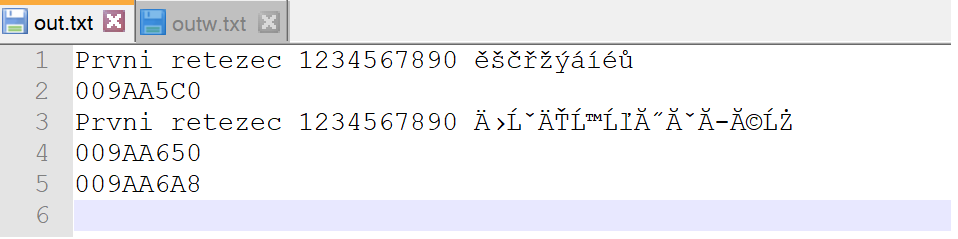
\includegraphics[width=\textwidth]{img/datastreams-outtxt.png}
\end{frame}



\begin{frame}[fragile]
\frametitle{wofstream - různé formáty textu}
\begin{yesblock}
\begin{lstlisting}
wofstream outputFile{ "outw.txt" };
// char
outputFile << "Prvni retezec 1234567890 ěščřžýáíéů" << endl;
// wchar_t
outputFile << L"Prvni retezec 1234567890 ěščřžýáíéů" << endl;
// utf-8 (char)
outputFile << u8"Prvni retezec 1234567890 ěščřžýáíéů" << endl;
// utf-16 (char16_t)
outputFile << u"Prvni retezec 1234567890 ěščřžýáíéů" << endl;
// utf-32 (char32_t)
outputFile << U"Prvni retezec 1234567890 ěščřžýáíéů" << endl;
outputFile.close();
\end{lstlisting}
\end{yesblock}
\end{frame}


\begin{frame}[fragile]
\begin{block}{}
Náhled v režimu ANSI (cp1250)
\begin{itemize}
\item korektně není zapsán žádný řetězec!
\item i u \lstinline|wchar_t| došlo k ořezu diakritických znaků
\end{itemize}
\end{block}
\vskip 1ex
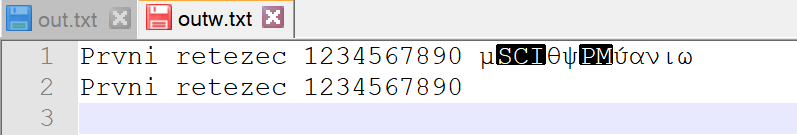
\includegraphics[width=\textwidth]{img/datastreams-outwtxt.png}
\end{frame}



\begin{frame}[fragile]
\frametitle{basic\_ofstream<char16\_t> - různé formáty textu}
\begin{yesblock}
\begin{lstlisting}
// utf-16 (char16_t)
std::basic_ofstream<char16_t> outputFile{ "out16.txt" };
outputFile << u"Prvni retezec 1234567890 ěščřžýáíéů" << endl;
outputFile.close();
\end{lstlisting}
\end{yesblock}
\end{frame}


\begin{frame}[fragile]
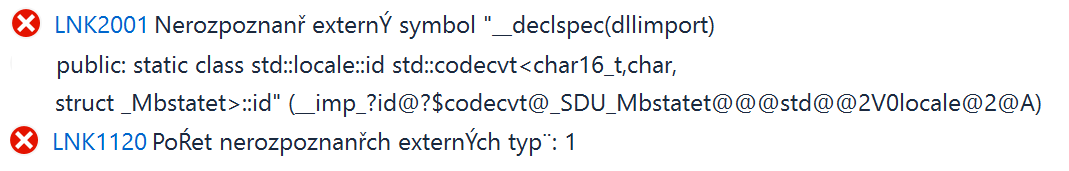
\includegraphics[width=\textwidth]{img/datastreams-char16terror.png}
\end{frame}

\begin{frame}[fragile]
\begin{block}{}
\begin{itemize}
\item V rámci paměti lze používat řetězce v kódování nativním kódování, UTF-8, UTF-16, UTF-32
\item V prostředí VS lze do souboru pouze zapisovat v nativním kódováním nebo v UTF-8
\end{itemize}
\end{block}
\end{frame}





\pkapitola{Binární soubory}




\begin{frame}[fragile]
\frametitle{Zápis binárního souboru -- struktura}
\begin{yesblock}
\begin{lstlisting}
struct JednoduchaStruktura {
	int a;
	int b;
	int c;
};

void testZapisACteniBinarne() {
	JednoduchaStruktura abc{ 1, 2, 3 };
	
	ofstream binFile{ "out.bin" };
	binFile.write((const char*)&abc, sizeof abc);
	binFile.close();
}

\end{lstlisting}
\end{yesblock}
\end{frame}


\begin{frame}[fragile]

\begin{block}{}
Náhled v HEX editoru
\begin{itemize}
\item \lstinline|sizeof(int) == 4| 
\item \lstinline|sizeof(JednoduchaStruktura) == 3*4 == 12|
\item OK
\item Pozor na přenos souboru na jinou platformu -- pořadí bajtů ve skupině je nyní little-endian
\begin{itemize}
\item Na systému big-endian by byly načteny hodnoty 16 777 216, 33 554 432, 50 331 648
\end{itemize}
\end{itemize}
\end{block}
\vskip 1ex
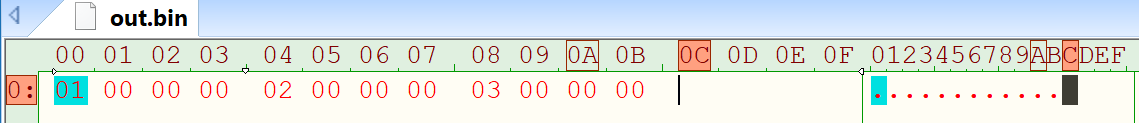
\includegraphics[width=\textwidth]{img/datastreams-bin1.png}
\end{frame}










\begin{frame}[fragile]
\frametitle{Zápis binárního souboru -- struktura}
\begin{yesblock}
\begin{lstlisting}
struct SlozitejsiStruktura {
	JednoduchaStruktura& ref;
	JednoduchaStruktura* ptr;
};

void testZapisACteniBinarne() {
	JednoduchaStruktura abc{ 1, 2, 3 };
	SlozitejsiStruktura structure{ abc, &abc };

	ofstream binFile{ "out.bin" };
	binFile.write((const char*)&structure, sizeof structure);
	binFile.close();
}
\end{lstlisting}
\end{yesblock}
\end{frame}


\begin{frame}[fragile]

\begin{block}{}
Náhled v HEX editoru
\begin{itemize}
\item \lstinline|sizeof(JednoduchaStruktura) == 12|
\item Velikost souboru == 8
\item Není OK
\item Reference i ukazatele jsou v paměti reprezentovány stejně
\begin{itemize}
\item Ukazatel (32/64 bitové číslo) na adresu do paměti
\item Binární zápis pouze zapíše hodnotu (tj. tu adresu), kterou ve struktuře přečte
\end{itemize}
\end{itemize}
\end{block}
\vskip 1ex
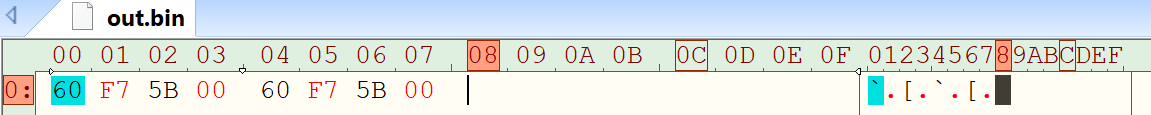
\includegraphics[width=\textwidth]{img/datastreams-bin2.png}
\end{frame}









\begin{frame}[fragile]
\frametitle{Zápis binárního souboru -- struktura}
\begin{yesblock}
\begin{lstlisting}
struct NevyrovnanaStruktura {
	char a;
	int b;
	char c;
	double d;
};

void testZapisACteniBinarne() {
	NevyrovnanaStruktura structure{ 0x99, 0x12345678, 0x99, 3.14};

	ofstream binFile{ "out.bin" };
	binFile.write((const char*)&structure, sizeof structure);
	binFile.close();
}
\end{lstlisting}
\end{yesblock}
\end{frame}


\begin{frame}[fragile]

\begin{block}{}
Náhled v HEX editoru
\begin{itemize}
\item \lstinline|sizeof(char)+sizeof(int)+sizeof(char)+sizeof(double) == 1+4+1+8 == 14|
\item Velikost souboru == 24
\item OK? Proč je větší?
\item Kompilátor automaticky zarovnává struktury (a třídy) v paměti, tak aby procesor přistupoval k adresám, které jsou násobky 4/8 bajtů a bylo dosaženo vyššího výkonu
\begin{itemize}
\item Stejný program bude strukturu znovu schopen načíst.
\item Stejný program zkompilovány jiným kompilátorem může na načítání selhat!
\end{itemize}

\end{itemize}
\end{block}
\vskip 1ex
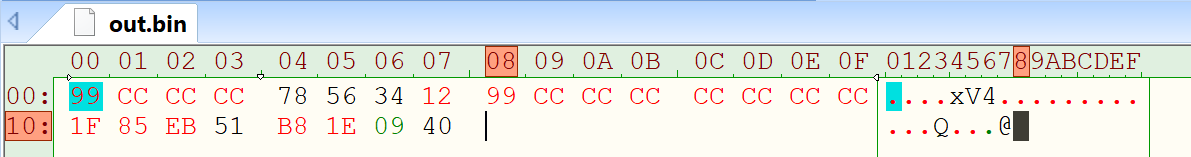
\includegraphics[width=\textwidth]{img/datastreams-bin3.png}
\end{frame}









\begin{frame}[fragile]
\frametitle{Zápis binárního souboru -- struktura}
\begin{yesblock}
\begin{lstlisting}
struct Struktura {
	string retezec;
};

void testZapisACteniBinarne() {
	Struktura structure{ "ahoj svete" };

	ofstream binFile{ "out.bin" };
	binFile.write((const char*)&structure, sizeof structure);
	binFile.close();
}
\end{lstlisting}
\end{yesblock}
\end{frame}


\begin{frame}[fragile]

\begin{block}{}
Náhled v HEX editoru
\begin{itemize}
\item Velikost souboru == 29
\item OK? Proč je to tolik?
\item Je to třída a nese nějaké atributy navíc, ale jinak to jde zapsat i načíst

\end{itemize}
\end{block}
\vskip 1ex
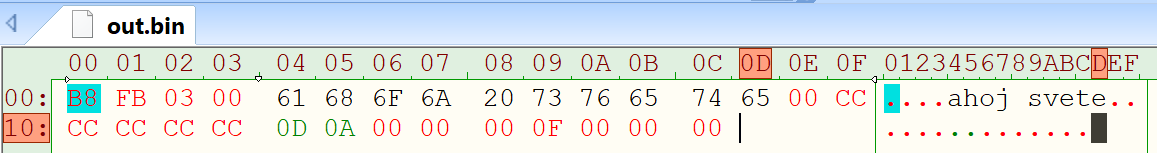
\includegraphics[width=\textwidth]{img/datastreams-bin4.png}
\end{frame}








\begin{frame}[fragile]
\frametitle{Zápis binárního souboru -- struktura}
\begin{yesblock}
\begin{lstlisting}
struct Struktura {
	string retezec;
};

void testZapisACteniBinarne() {
	Struktura structure{ "ahoj svete, dneska je moc pekne!" };

	ofstream binFile{ "out.bin" };
	binFile.write((const char*)&structure, sizeof structure);
	binFile.close();
}
\end{lstlisting}
\end{yesblock}
\end{frame}


\begin{frame}[fragile]

\begin{block}{}
Náhled v HEX editoru
\begin{itemize}
\item Velikost souboru == 28
\item OK? Ne!
\item Text není uložen v souboru!

\end{itemize}
\end{block}
\vskip 1ex
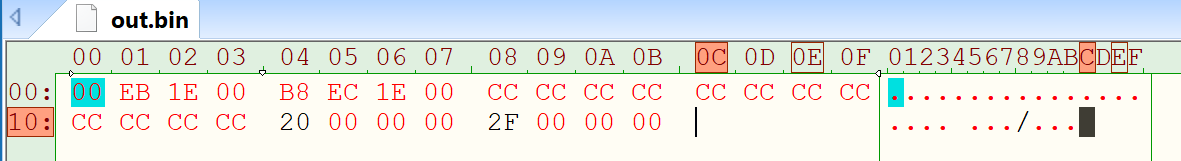
\includegraphics[width=\textwidth]{img/datastreams-bin5.png}
\end{frame}

\begin{frame}[fragile]
\begin{block}{Implementace std::string v knihovně}
\begin{itemize}
\item Liší se dle autora knihovny
\item Někde je využívána přímo dynamicky alokovaná paměť
\item Někde je používán hybridní přístup
\begin{itemize}
\item Pro krátké řetězce (do 16 znaků) je přímo ve třídě staticky alokované pole, kam se uloží znaky
\item Delší řetězce vyžadují alokaci samostatného paměťového bloku a do struktury je uložen ukazatel
\item[] 
\item Tento přístup umožňuje předcházet dvojí alokaci paměti pro krátké řetězce
\item Je využíván i v rámci knihovny od Microsoftu
\end{itemize}
\end{itemize}
\end{block}
\end{frame}


\begin{frame}[fragile]

\begin{block}{Zápis struktur do souboru}
Lze při splnění podmínek:
\begin{itemize}
\item struktura neobsahuje referenční nebo ukazatelové atributy
\item program má ošetřenou přenositelnost (little-endian/big-endian) pro případ přesunu na jinou platformu
\item program má ošetřené zarovnání struktur pro případ přesunu na jiný kompilátor/platformu
\end{itemize}
\vskip 1ex
Nelze tedy přímo zapisovat struktury u kterých si nejsme jisti splněním těchto podmínek (\lstinline|std::vector, std::string|, \ldots)

\end{block}
\end{frame}



\zkouskove


%\hkapitola{Následující části jsou ještě v~hodně rozpracované verzi}

%\hkapitola{Přetěžování operátorů}

\begin{frame}[fragile]
\vfill
\begin{bitemize}{Přetěžování operátorů}
\item podobně jako C++ lze v C\# přetěžovat operátory u svých objektových typů
\item množina přetížitelných operátorů je oproti C++ menší
\item syntax a pravidla pro přetěžování jsou striktnější a snaží se zamezit problémům
\begin{itemize}
\item např. není možné přetížit == bez přetížení !=
\end{itemize}

\end{bitemize}
\vfill
\begin{bitemize}{Přetížitelné operátory}
\item \lstinline|- ! ~ ++ -- true false|
\item \lstinline|- * / % & ^ | | \lstinline| << >> == != > < >= <=|
\item konverzní operátory
\item \lstinline|[ ]| (indexery)
\end{bitemize}
\vfill
\end{frame}


\nezkouskove

\begin{frame}[fragile]
\frametitle{Přetížení oprerátoru}
\vfill
\begin{noteblock}{}
\begin{lstlisting}
public static typ operator symbol ( parametry ) tělo
\end{lstlisting}
\end{noteblock}
\vfill
\begin{bitemize}{}
\item parametry
\begin{itemize}
\item unární operátor -- jeden parametr
\item binární operátor -- dva parametry
\end{itemize}

\item logické dvojice -- vždy je nutné přetížit oba operátory naráz
\begin{itemize}
\item \lstinline|== !=|
\item \lstinline|< >|
\item \lstinline|<= >=|
\item \lstinline|true false|
\end{itemize}

\item inkremetace/dekremetace se přetěžuje jednou metodou, kompilátor ji automaticky použije pro prefixovou i postfixovou variantu
\item operátory \lstinline|true,false| umožňují dát objekt přímo do výrazů očekávající logickou hodnotu (\lstinline|if, while, ...|)

\end{bitemize}
\vfill
\end{frame}




\begin{frame}[fragile]
\begin{yesblock}
\begin{lstlisting}
class Complex
{
    public double Re { get; set; }
    public double Im { get; set; }

    public static Complex operator +(Complex a, Complex b)
    {
        return new Complex()
        {
            Re = a.Re + b.Re,
            Im = a.Im + b.Im
        };
    }

    // ...
}
\end{lstlisting}
\end{yesblock}
\end{frame}




\begin{frame}[fragile]
\begin{yesblock}
\begin{lstlisting}
    public static bool operator ==(Complex a, Complex b)
    {
        return a.Re == b.Re && a.Im == b.Im;
    }

    public static bool operator !=(Complex a, Complex b)
    {
        return a.Re != b.Re || a.Im != b.Im;
    }
\end{lstlisting}
\end{yesblock}
\end{frame}




\begin{frame}[fragile]
\begin{yesblock}
\begin{lstlisting}
    public static Complex operator ++(Complex c)
    {
        return new Complex()
        {
            Re = c.Re + 1,
            Im = c.Im
        };
    }
\end{lstlisting}
\end{yesblock}
\end{frame}




\begin{frame}[fragile]
\frametitle{Přetížení oprerátoru -- konverzní operátory}
\vfill
\begin{noteblock}{}
\begin{lstlisting}
public static implicit operator cílovýTyp ( zdrojovýTyp parametr ) tělo
public static explicit operator cílovýTyp ( zdrojovýTyp parametr ) tělo
\end{lstlisting}
\end{noteblock}
\vfill
\begin{bitemize}{}
\item není možné zároveň definovat pravidla pro implicitní a explicitní konverzi
\item kompilátor tyto operátory volá při výrazech:
\begin{itemize}
\item implicitní
\begin{itemize}
\item \lstinline|cílovýTyp proměnná = objektZdrojovéhoTypu|
\end{itemize}

\item explicitní
\begin{itemize}
\item \lstinline|cílovýTyp proměnná  = (cílovýTyp)objektZdrojovéhoTypu|
\end{itemize}
\end{itemize}

\end{bitemize}
\vfill
\end{frame}




\begin{frame}[fragile]
\vfill
\begin{yesblock}
\begin{lstlisting}
    public static explicit operator double(Complex c)
    {
        return c.Re;
    }
\end{lstlisting}
\end{yesblock}
\vfill
\begin{yesblock}
\begin{lstlisting}
Complex c = new Complex()
{
    Re = 10,
    Im = 5
};

double realPart = (double)c;
Console.WriteLine($"{realPart}");
\end{lstlisting}
\end{yesblock}
\vfill
\end{frame}






\zkouskove

\begin{frame}[fragile]
\frametitle{Indexery}
\vfill
\begin{bitemize}{}
\item definují přetížení operátoru \lstinline|[ ]| pro přístup k prvkům/datům
\item definují se jako \textbf{instanční} (nestatické) \textbf{vlastnosti}
\end{bitemize}
\vfill
\begin{noteblock}{}
\begin{lstlisting}
[modifikátor] návratovýTyp this [ seznamParametrů ] deklaracePřístupovýchMetod
\end{lstlisting}
\end{noteblock}
\vfill
\begin{yesblock}
\begin{lstlisting}
class IndexerExample
{
    readonly int[] values = new int[] { 1, 2, 3, 4, 5, 6, 7, 8, 9, 10 };

    public int this[int index]
    {
        get => values[index];
    }
}
\end{lstlisting}
\end{yesblock}
\vfill
\end{frame}


\begin{frame}[fragile]
\frametitle{Indexery}
\vfill
\begin{bitemize}{}
\item je možné definovat několik různých přetížení indexerů s různými parametry
\item rozhraní mohou definovat indexery
\item indexer může data číst (\lstinline|get|) / zapisovat (\lstinline|set|) nebo provádět obojí
\end{bitemize}
\vfill
\begin{yesblock}
\begin{lstlisting}
var indexer = new IndexerExample();
int numberThree = indexer[2];
\end{lstlisting}
\end{yesblock}
\vfill
\end{frame}



\begin{frame}[fragile]
\begin{yesblock}
\begin{lstlisting}
class Table
{
    public Row this[int row]
    {
        get => GetRow(row);
        set => SetRow(row, value);
    }

    public string this[string identifier]
    {
        get => GetMetadata(identifier);
    }

    // ...

}
\end{lstlisting}
\end{yesblock}
\end{frame}
%\hkapitola{STL}

\begin{frame}[fragile]
\begin{block}{STL -- Standard Template Library}
\begin{itemize}
\item představuje generickou knihovnu pro správu a zpracování dat
\item jednotlivé komponenty jsou šablony
\item základní komponenty jsou
\begin{itemize}
\item kontejnery -- slouží pro ukládání a organizaci dat
\item algoritmy -- obecné algoritmy pro zpracování dat
\item iterátory -- obecné \uv{rozhraní} mezi kontejnery a algoritmy
\item pomocné funkční objekty, adaptéry, bindery, \ldots
\end{itemize}
\end{itemize}
\end{block}


\begin{block}{Funkční objekt}
\begin{itemize}
\item vylepšení obyčejné funkce
\item objekt s přetíženým operátorem \lstinline|()|
\begin{itemize}
\item lze volat jako funkci
\item má atributy (stav)
\end{itemize}
\item od C++11 lze výhodně využívat lambda výrazy
\item v STL existuje řada univerzálních funkčních objektů a adaptérů
\end{itemize}
\end{block}
\end{frame}





\begin{frame}[fragile]
\frametitle{Kontejnery}

\begin{block}{}
\begin{itemize}
\item slouží pro ukládání dat
\item standard definuje rozhraní a složitost operací (není definována konkrétní fyzická datová struktura)
\end{itemize}
\end{block}
\vskip -1.5ex
\begin{block}{}
\begin{itemize}
\item posloupnosti -- data nemají vlastní identifikátor (klíč)
\begin{itemize}
\item \lstinline|array|\cpp{11}
\item \lstinline|vector|
\item \lstinline|deque|
\item \lstinline|list|, \lstinline|forward_list|\cpp{11}
\item adaptéry -- \lstinline|stack|, \lstinline|queue|, \lstinline|priority_queue|
\end{itemize}
\item asociativní kontejnery -- data mají vlastní identifikátor (klíč)
\begin{itemize}
\item \lstinline|set|, \lstinline|multiset|
\item \lstinline|map|, \lstinline|multimap|
\item hashovací kontejnery\cpp{11} (\lstinline|unordered_{set,map,multiset,multimap}|)
\end{itemize}
\end{itemize}
\end{block}
\end{frame}






\begin{frame}[fragile]
\frametitle{Iterátory}
\begin{block}{}
\begin{itemize}
\item představují jednotné rozhraní pro procházení dat v libovolném kontejneru
\item vycházejí z ukazatelů a logiky jejich použití (ukazatel na pole je v~zásadě iterátor)
\item obvykle realizovány jako objekty s přetíženými operátory
\item definováno několik kategorií iterátorů dle požadovaných operací
\end{itemize}
\end{block}

\begin{block}{}
\begin{itemize}
\item \lstinline|InputIterator| -- čtou data z kontejneru
\begin{itemize}
\item \lstinline|ForwardIterator|
\item \lstinline|BidirectionalIterator|
\item \lstinline|RandomAccessIterator|
\item \lstinline|ContiguousIterator|\cpp{17}
\end{itemize}
\item \lstinline|OutputIterator| -- zapisují data do kontejneru
\end{itemize}
\end{block}
\end{frame}






\begin{frame}[fragile]
\frametitle{Algoritmy}
\begin{block}{}
\begin{itemize}
\item zpracovávají data
\begin{itemize}
\item vyhledávají
\item mažou
\item upravují
\item obecně zpracovávají prvky
\item řadí
\item \ldots
\end{itemize}
\item pracují s obecnými daty a s obecnými zdrojy dat
\begin{itemize}
\item tvar dat je libovolný (int, string, složitý objekt)
\item zdroj dat je libovolný (používají se iterátory)
\item konkrétní zpracování dat je definováno pomocí operátorů nebo funkčních objektů
\end{itemize}
\end{itemize}
\end{block}
\end{frame}



\kapitola{C++11 a STL, kontejnery, iterátory, algoritmy}

\begin{frame}[fragile]
\frametitle{auto}
\begin{block}{}
\begin{itemize}
\item \lstinline|auto| umožňuje místo psaní konkrétního datového typu nechat typ odvodit kompilátor. 
\item stále se jedná o silné typování, typ proměnné není možné později změnit
\item lze s výhodou využít v mnoha situacích v následující práci s STL
\item \lstinline|auto| je možné dále specifikovat modifikátory
\end{itemize}
\end{block}	

\begin{yesblock}
\lstinline|Object obj;|
\begin{itemize}
\item \lstinline|auto v = obj; // Object v|
\item \lstinline|const auto v = obj; // const Object v|
\item \lstinline|auto& v = obj; // Object& v|
\item \lstinline|const auto& v = obj; // const Object& v|
\end{itemize}
\end{yesblock}
\end{frame}

\begin{frame}[fragile]
\frametitle{initializer\_list}
\begin{block}{}
\begin{itemize}
\item kontejnery je možné inicializovat výčtem hodnot pomocí inicializačních seznamů
\item jde o rozšíření syntaxe uniform initialization
\end{itemize}
\end{block}

\begin{yesblock}
\begin{itemize}
\item  \lstinline|vector<int> vect {10, 15, 20, 25, 30};|
\item  \lstinline|vector<int> vect = {10, 15, 20, 25, 30};|
\end{itemize}
\end{yesblock}	
\end{frame}





\begin{frame}[fragile]
\frametitle{Lambda výrazy -- anonymní funkce}
\begin{noteblock}{}
\begin{center}
[] () \{\}
\end{center}
\end{noteblock}
\end{frame}

\begin{frame}[fragile]
\frametitle{Lambda výrazy -- anonymní funkce}
\begin{noteblock}{}
\begin{center}
[ zachycení vnějších proměnných ] ( parametry funkce ) \{ tělo funkce \}
\end{center}
\end{noteblock}
\end{frame}

\begin{frame}[fragile]
\frametitle{Lambda výrazy -- zachycení vnějších proměnných}
\begin{yesblock}
\begin{lstlisting}
int x = 10;

// auto lambda0 = []() { return x; }; // nejde - x není definováno v anonymní funkci

// zachycení hodnotou
auto lambda1 = [x]() { return x; }; // ++x - nejde (je read only)
cout << lambda1(); // x = 10; out = 10;

// zachycení referencí (odkazem)
auto lambda2 = [&x]() { return ++x; };
cout << lambda2(); // x = 11; out = 11;
\end{lstlisting}
\end{yesblock}
\end{frame}


\begin{frame}[fragile]
\frametitle{Lambda výrazy -- parametry funkce}
\begin{yesblock}
\begin{lstlisting}
auto lambda0 = []() { return 1; };
cout << lambda0() << endl; // 1

auto lambda1 = [](int x) { return 2 * x; };
cout << lambda1(10) << endl; // 20

auto lambda2 = [](int x, int y, double t) { return x + y; };
cout << lambda2(10, 20, 3.1415) << endl; // 30
\end{lstlisting}
\end{yesblock}
\end{frame}

\begin{frame}[fragile]
\begin{noteblock}{specifikace návratového typu}
\begin{center}
[ ] ( ) -> návratový\_typ \{ \}
\end{center}
\end{noteblock}

\begin{noteblock}{mutable}
\begin{center}
[ ] ( ) \textit{mutable} -> návratový\_typ \{ \}
\end{center}

Umožňuje měnit vnější hodnoty zachycené hodnotou (změna se projeví pouze v těle lambdy).
\end{noteblock}

\begin{block}{zachycení vnejších hodnot}
\begin{itemize}
\item \lstinline |[=]| -- vše hodnotou
\item \lstinline |[&]| -- vše odkazem
\item \lstinline |[x, &]| -- x hodnotou, zbytek odkazem
\item \lstinline |[this]| -- zachycení this v objektu 
\end{itemize}
\end{block}
\end{frame}

\begin{frame}[fragile]
\frametitle{Předávání / uchování anonymních funkcí}
\begin{yesblock}
\begin{lstlisting}
// použitím auto
auto lambda1 = [](int value){ return value = 1; }

// použitím std::function<>
std::function<int(int)> = [](int value){ return value = 1;}
\end{lstlisting}
\end{yesblock}

\begin{block}{std::function<>}
\begin{itemize}
\item šablona s proměnným počtem parametrů
\item parametry ve tvaru \lstinline|result(param1, param2, ...)|
\begin{itemize}
\item \lstinline|function<int()>| -- funkce bez parametrů, vrací int
\item \lstinline|function<void(int)>| -- funkce s jedním int parametrem, vrací void
\item \lstinline|function<int(int)>| -- funkce s jedním int parametrem, vrací int
\item \lstinline|function<int(int, int)>| -- funkce se dvěma int parametry, vrací int
\end{itemize}

\end{itemize}
\end{block}
\end{frame}


\begin{frame}[fragile]
%\frametitle{std::function}
\begin{block}{std::function<>}
\begin{itemize}
\item umožňuje uchovávat i ukazatel na libovolnou funkci nebo metodu
\end{itemize}
\end{block}

\begin{yesblock}
\begin{lstlisting}
std::function<void(Citac&, int)> fptr = &Citac::nastavAtribut;
	
Citac citac{};
fptr(citac, 10);

\end{lstlisting}
\end{yesblock}
\end{frame}







% 07
%\hkapitola{Kontejnery}

\begin{frame}[fragile]
\frametitle{Kontejnery}

\begin{block}{}
\begin{itemize}
\item slouží k ukládání dat (koncept podobný s kolekcemi v Javě)
\item různé druhy kontejnerů dle požadovaného použití
\item dodržují jednotné rozhraní
\item dvě základní skupiny:
\begin{itemize}
\item posloupnosti
\item asociativní kontejnery
\end{itemize}
\end{itemize}
\end{block}
\end{frame}






\begin{frame}[fragile]
\begin{block}{Přehled kontejnerů}
\begin{itemize}
\item posloupnosti -- data nemají vlastní identifikátor (klíč)
\begin{itemize}
\item \lstinline|array|\cpp{11}
\item \lstinline|vector|
\item \lstinline|deque|
\item \lstinline|list|, \lstinline|forward_list|\cpp{11}
\item adaptéry -- \lstinline|stack|, \lstinline|queue|, \lstinline|priority_queue|
\end{itemize}
\item asociativní kontejnery -- data mají vlastní identifikátor (klíč)
\begin{itemize}
\item \lstinline|set|, \lstinline|multiset|
\item \lstinline|map|, \lstinline|multimap|
\item hashovací kontejnery\cpp{11} (\lstinline|unordered_{set,map,multiset,multimap}|)
\end{itemize}
\end{itemize}
\end{block}
\end{frame}









\begin{frame}[fragile]
\begin{block}{Základní vlastnosti kontejnerů}
\begin{itemize}
\item realizovány jako šablony tříd, pomocí parametrů šablony lze nastavit
\begin{itemize}
\item typ ukládaných dat,
\item typ alokátoru (specifikuje práce s pamětí),
\item způsob porovnání dat u asociativních kontejnerů,
\item způsob hashování u hashovacích kontejnerů
\end{itemize}
\end{itemize}
\end{block}

\begin{yesblock}
\begin{lstlisting}[basicstyle=\small]
std::vector<Kocka> 
	kontejnerKocek{};

std::map<string, Kocka> 
	mapaKocekPodleJejichJmena{};

std::set<Kocka, RazeniKocekPodleBarvy>
	mnozinaKocekRazenaDleBarvy{};

std::vector<Kocka, KockoAlokator> 
	zvlastneAlokovanyVektorKocek{};
\end{lstlisting}
\end{yesblock}
\end{frame}








\begin{frame}[fragile]
\begin{block}{Základní vlastnosti kontejnerů\ldots}
\begin{itemize}
\item kontejnery poskytují hodnotovou sémantiku
\begin{itemize}
\item data (objekty/primitivní hodnoty) jsou kopírovány do vnitřního úložiště kontejneru
\item nejedná se o reference na původní umístění dat
\end{itemize}
\end{itemize}
\end{block}


\begin{noblock}
\begin{lstlisting}
std::vector<Kocka&> kontejnerReferenciNaKocky{};
\end{lstlisting}
\end{noblock}

\begin{yesblock}
\begin{lstlisting}
std::vector<Kocka> kontejnerKocek{};
// od C++11 lze použít std::reference_wrapper
// kontejner pak obsahuje objekty, které uchovávájí reference 
std::vector<std::reference_wrapper<Kocka>> 
	kontejnerReferenciNaKocky{};
\end{lstlisting}
\end{yesblock}
\end{frame}




\begin{frame}[fragile]
\begin{block}{Základní vlastnosti kontejnerů\ldots}
\begin{itemize}
\item operace nejsou bezpečné
\begin{itemize}
\item je nutné hlídat splnění požadavků na parametry jednotlivých operací
\item v době kompilace není možné otestovat zcela správnost volání
\end{itemize}

\item pro realizaci obecných algoritmů kontejnery zveřejňují několik základních datových typů
\begin{itemize}
\item \lstinline|value_type| -- typ ukládaných hodnot
\item \lstinline|key_type| -- typ klíče
\item \lstinline|pointer (const_pointer)| -- typ ukazatele na typ uložené hodnoty
\item \lstinline|reference (const_reference))| -- typ reference na typ uložené hodnoty
\item \lstinline|iterator (const_iterator)| -- typ iterátoru
\item \lstinline|reverse_iterator (const_reverse_iterator)| -- typ reverzního iterátoru
\end{itemize}
\end{itemize}
\end{block}

\begin{yesblock}
\begin{lstlisting}
std::vector<int>::value_type intPromenna = ...;
std::vector<Kocka>::pointer ukazatelNaKockuPromenna = ...;
\end{lstlisting}
\end{yesblock}
\end{frame}







\begin{frame}[fragile]
\frametitle{Základní operace kontejnerů}

\begin{block}{Konstrukce kontejneru}
\begin{itemize}
\item \lstinline|Kontejner()| -- vytvoření prázdného kontejneru
\item \lstinline|Kontejner(Kontejner k)|, \lstinline|operator=| -- zkopírování obsahu stejného typu kontejneru
\item \lstinline|Kontejner(Iterator begin, Iterator end)| -- vytvoření kontejneru z dat dle iterátorů
\item \lstinline|Kontejner(initializer_list il)| -- vytvoření pomocí \lstinline|initializer_list|
\end{itemize}
\end{block}

\begin{yesblock}
\begin{lstlisting}
std::vector<int> prazdnyVektor{};
std::vector<int> vektorInitializerList = {1, 2, 3, 4, 5};
std::vector<int> vektorInitializerList2{1, 2, 3, 4, 5};
std::vector<int> kopieVektoru = vektorInitializerList;
\end{lstlisting}
\end{yesblock}
\end{frame}




\begin{frame}[fragile]
\frametitle{Základní operace kontejnerů\ldots}

\begin{block}{Počet prvků v kontejneru}
\begin{itemize}
\item \lstinline|size()| -- vrací počet položek v kontejneru
\item \lstinline|empty()| -- vrací \lstinline|true|, pokud je kontejner prázdný
\end{itemize}
\end{block}

\begin{yesblock}
\begin{lstlisting}
std::vector<int> prazdnyVektor{};
bool jePrazdny = prazdnyVektor.empty();

if (prazdnyVektor.size() > 10)
	...
\end{lstlisting}
\end{yesblock}
\end{frame}





\begin{frame}[fragile]
\frametitle{Základní operace kontejnerů\ldots}

\begin{block}{Procházení kontejnerů (iterátory)}
\begin{itemize}
\item \lstinline|begin()| -- vrací iterátor ukazující na první prvek v kontejneru
\item \lstinline|end()| -- vrací iterátor ukazující za poslední prvek v kontejneru
\vskip 2ex
\item \lstinline|cbegin(), cend()| -- konstantní iterátory
\item \lstinline|rbegin(), rend()| -- reverzní iterátory

\end{itemize}
\end{block}

\begin{yesblock}
\begin{lstlisting}
std::vector<int> vektor{1, 2, 3, 4, 5};

for (std::vector<int>::iterator it = vektor.begin(); it != vektor.end(); ++it) {
	cout << *it << endl;
}
\end{lstlisting}
\end{yesblock}
\end{frame}



\begin{frame}[fragile]
\frametitle{Základní operace kontejnerů\ldots}
\begin{yesblock}
\begin{lstlisting}
std::vector<int> vektor{1, 2, 3, 4, 5};

for (auto it = vektor.begin(); it != vektor.end(); ++it) {
	cout << *it << endl;
}
\end{lstlisting}
\end{yesblock}

\begin{yesblock}
\begin{lstlisting}
std::vector<int> vektor{1, 2, 3, 4, 5};

// také lze s "auto"
for (int cislo : vektor) {
	cout << cislo << endl;
}
\end{lstlisting}
\end{yesblock}
\end{frame}







\begin{frame}[fragile]
\frametitle{Základní operace kontejnerů\ldots}
\begin{block}{Úpravy prvků v kontejneru}
\begin{itemize}
\item \lstinline|insert(pozice, prvek)| -- vloží prvek do kontejneru
\item \lstinline|erase(zacatek, konec)| -- odstraní vybrané prvky z kontejneru
\item \lstinline|clear()| -- odstrání všechny prvky z kontejneru
\end{itemize}
\end{block}
\end{frame}


\begin{frame}
% leva spodek prava vrsek
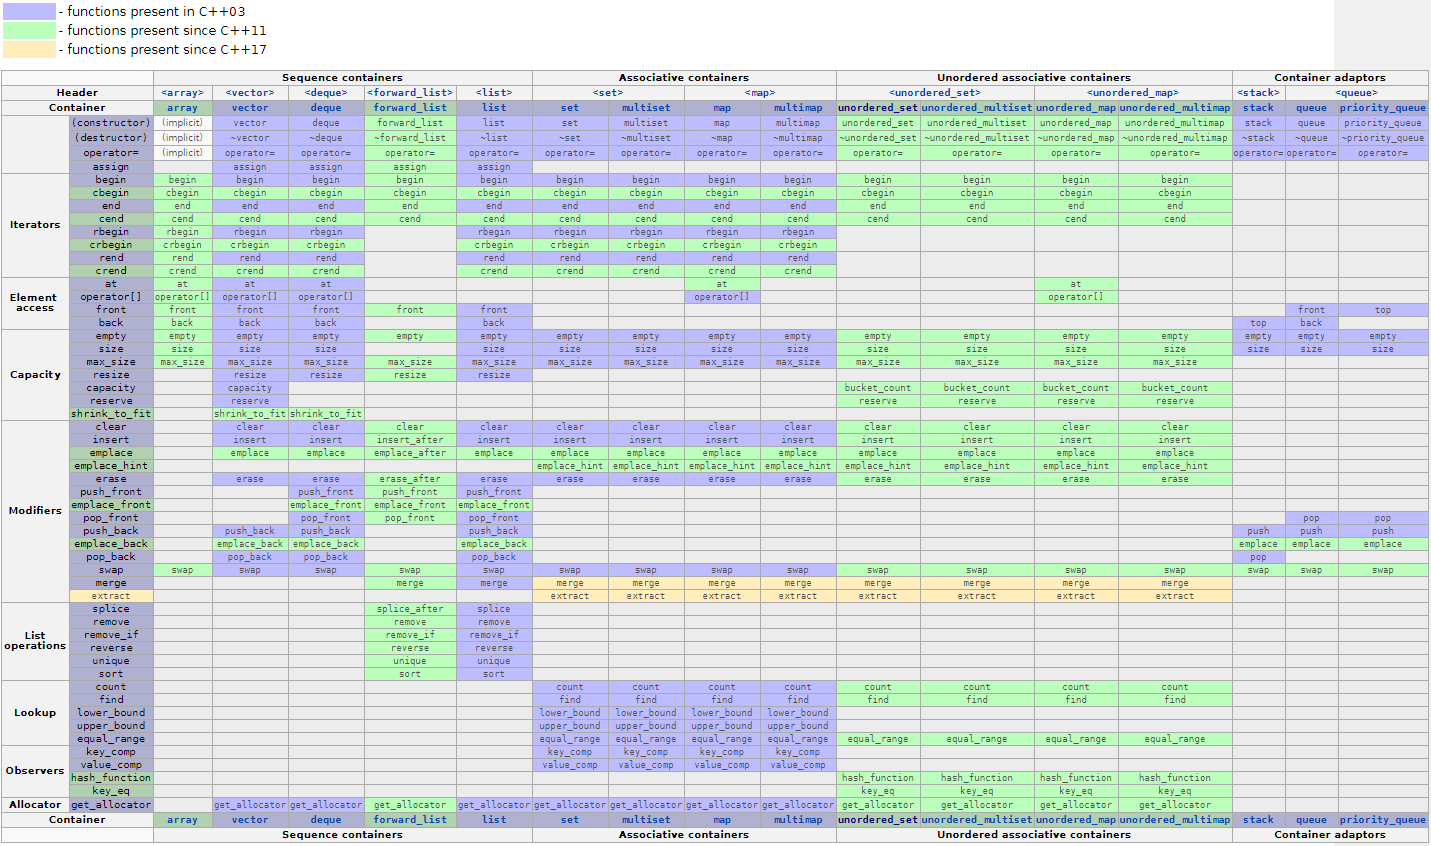
\includegraphics[width=\linewidth,clip,trim=0 6.3cm 15.5cm 0]{img/kontejnery-prehled-metod.png}
\end{frame}

\begin{frame}
% leva spodek prava vrsek
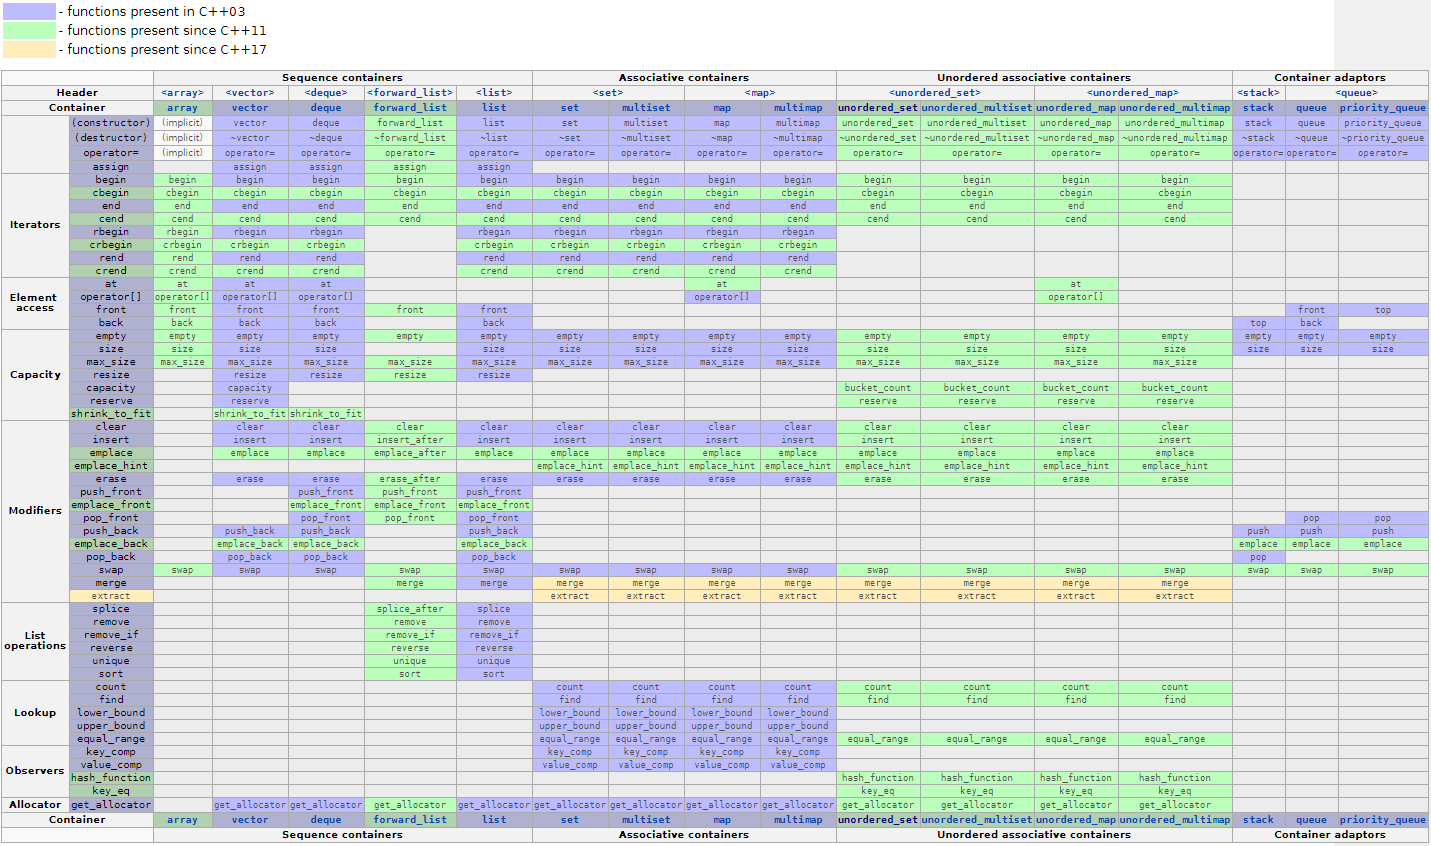
\includegraphics[width=\linewidth,clip,trim=0 0 15.5cm 15.9cm]{img/kontejnery-prehled-metod.png}
\end{frame}











\kapitola{Posloupnosti}

\begin{frame}[fragile]
\begin{block}{Přehled posloupností}
\begin{itemize}
\item \lstinline|array|\cpp{11} -- pole statické velikosti
\item \lstinline|vector| -- dynamicky alokované pole
\item \lstinline|deque| -- oboustranně dynamicky alokované pole
\item \lstinline|list| -- obousměrně zřetězený spojový seznam
\item \lstinline|forward_list|\cpp{11} -- jednosměrně zřetězený spojový seznam
\item adaptéry 
\begin{itemize}
\item \lstinline|stack| -- zásobník
\item \lstinline|queue| -- fronta
\item \lstinline|priority_queue| -- prioritní fronta
\end{itemize}
\end{itemize}
\end{block}
\end{frame}



\pkapitola{vector}

\begin{frame}[fragile]
\begin{block}{vector}
\begin{itemize}
\item \lstinline|#include <vector>|
\item šablona \lstinline|vector<TypDat, Alokator = vychozí>|
\item iterátor -- random access
\vskip 2ex
\item obvykle realizován jako dynamické pole
\vskip 2ex
\item poskytuje O(1) složitost čtení libovolného prvku
\item rychlé přidávání a odebírání prvků z konce vektoru
\item pomalá úprava prvků uprostřed vektoru
\end{itemize}
\end{block}
\end{frame}


\begin{frame}[fragile]
\begin{block}{vector}
\begin{itemize}
\item při úpravách pomalé realokace pole -- možnost rezervovat kapacitu vnitřního pole
\item \lstinline|vector.capacity()| -- vrací velikost interního pole
\item \lstinline|vector.reserve(velikost)| -- vyhradí paměť pro \lstinline|velikost| prvků
\item \lstinline|vector.resize(velikost)| -- změní počet prvků na \lstinline|velikost|, způsobuje smazání nebo přidání prvků!
\item \lstinline|vector.shrink_to_fit()|\cpp{11} -- zmenší vnitřní pole pouze na potřebnou velikost pro aktuální počet prvků
\end{itemize}
\end{block}
\end{frame}



\begin{frame}[fragile]
\frametitle{Vkládání hodnot}
\begin{yesblock}
\begin{lstlisting}
std::vector<int> v{};

// vložení hodnoty na konec
v.push_back(10);
// vložení hodnot na zvolené místo (iterátorem)
v.insert(v.end(), 20);

// konstrukce a vložení hodnoty na konci (C++11)
v.emplace_back(30);
// konstrukce a vložení hodnoty na zvoleném místě (C++11)
v.emplace(v.end(), 40);

for (auto item : v) { // foreach (C++11)
	cout << item << endl; 
}
// 10 20 30 40
\end{lstlisting}
\end{yesblock}
\end{frame}


\begin{frame}[fragile]
\frametitle{Vkládání hodnot -- objekt KomplexniCislo -- definice}
\begin{yesblock}
\begin{lstlisting}
struct KomplexniCislo {
	int real;
	int imag;

	KomplexniCislo() : real(0), imag(0) {}
	KomplexniCislo(int re, int im) : real(re), imag(im) {}
};

ostream& operator<<(ostream& os, const KomplexniCislo& kc) {
	os << kc.real << " + " << kc.imag << "i";
	return os;
}
\end{lstlisting}
\end{yesblock}
\end{frame}

\begin{frame}[fragile]
\frametitle{Vkládání hodnot -- objekt KomplexniCislo -- použití}
\begin{yesblock}
\begin{lstlisting}
std::vector<KomplexniCislo> v{};

v.push_back(KomplexniCislo{ 1, 0 });
v.insert(v.end(), KomplexniCislo{ 10, 0 });

v.emplace_back(1, 10);
v.emplace(v.end(), 5, 50);

vypis(v);
// 1 + 0i
// 10 + 0i
// 1 + 10i
// 5 + 50i
\end{lstlisting}
\end{yesblock}
\end{frame}


\begin{frame}[fragile]
\frametitle{Incializace pomocí initializer\_list}
\begin{yesblock}
\begin{lstlisting}
std::vector<KomplexniCislo> v{
	{1, 0},
	{10, 0},
	{1, 10},
	{5, 50}
};

vypis(v);
// 1 + 0i
// 10 + 0i
// 1 + 10i
// 5 + 50i
\end{lstlisting}
\end{yesblock}
\end{frame}

\begin{frame}[fragile]
\frametitle{Mazání prvků pomocí erase}
\begin{yesblock}
\begin{lstlisting}
std::vector<KomplexniCislo> v{
	{1, 0},
	{10, 0},
	{1, 10},
	{5, 50}
};

auto it = v.begin() + 1;
v.erase(it);

vypis(v);
// 1 + 0i
// - 10 + 0i - smazán
// 1 + 10i
// 5 + 50i
\end{lstlisting}
\end{yesblock}
\end{frame}

\begin{frame}[fragile]
\frametitle{Mazání prvků pomocí erase -- hromadné mazání}
\begin{yesblock}
\begin{lstlisting}
std::vector<KomplexniCislo> v{
	{1, 0},
	{10, 0},
	{1, 10},
	{5, 50}
};

auto it1 = v.begin() + 1;
auto it2 = v.begin() + 3;
v.erase(it1, it2);

vypis(v);
// 1 + 0i
// - 10 + 0i - smazán
// - 1 + 10i - smazán
// 5 + 50i
\end{lstlisting}
\end{yesblock}
\end{frame}




\begin{frame}[fragile]
\frametitle{Přístup k prvkům}
\begin{yesblock}
\begin{lstlisting}
std::vector<KomplexniCislo> v{
	{ 1, 0 },
	{ 10, 0 },
	{ 1, 10 },
	{ 5, 50 }
};

KomplexniCislo kc1 = v[0]; // 1 + 0i
KomplexniCislo kc2 = *v.begin(); // 1 + 0i
KomplexniCislo kc3 = *(v.begin() + 1); // 10 + 0i
KomplexniCislo kc4 = v.at(2); // 1 + 10i
KomplexniCislo kc5 = v.front(); // 1 + 0i
KomplexniCislo kc6 = v.back(); // 5 + 50i
KomplexniCislo kc7 = *v.rbegin(); // 5 + 50i
\end{lstlisting}
\end{yesblock}
\end{frame}






\pkapitola{deque}

\begin{frame}[fragile]
\begin{block}{deque}
\begin{itemize}
\item \lstinline|#include <deque>|
\item šablona \lstinline|deque<TypDat, Alokator = vychozí>|
\item iterátor -- random access
\vskip 2ex
\item obvykle realizován jako pole polí
\vskip 2ex
\item oproti vektoru zrychluje přidávání a odebírání prvků ze začátku kontejneru
\end{itemize}
\end{block}
\end{frame}


\begin{frame}[fragile]
\frametitle{Přidávání prvků na začátek/konec}
\begin{yesblock}
\begin{lstlisting}
std::deque<KomplexniCislo> d{
	{ 1, 0 },
	{ 10, 0 },
	{ 1, 10 },
	{ 5, 50 }
};

d.push_front({ 0, 0 });
// nebo také: d.emplace_front(0, 0);
d.push_back({ 100, 100 });
// 0 + 0i
// 1 + 0i
// 10 + 0i
// 1 + 10i 
// 5 + 50i
// 100 + 100i
\end{lstlisting}
\end{yesblock}
\end{frame}











\pkapitola{list}

\begin{frame}[fragile]
\begin{block}{list}
\begin{itemize}
\item \lstinline|#include <list>|
\item šablona \lstinline|list<TypDat, Alokator = vychozí>|
\item iterátor -- bidirectional
\vskip 2ex
\item obvykle realizován jako obousměrně zřetězený spojový seznam
\vskip 2ex
\item O(1) složitost libovolné atomické úpravy spojového seznamu
\item pomalé vyhledávání prvku
\item iterátor zůstává v platnosti i při změnách v seznamu
\end{itemize}
\end{block}
\end{frame}




\begin{frame}[fragile]
\begin{block}{Operace nad spojovým seznamem}
\begin{itemize}
\item \lstinline|l.remove(hodnota)| -- odebere všechny prvky s danou hodnotou
\item \lstinline|l.remove_if(podminka)| -- odebere všechny prvky splňující podmínku


\item \lstinline|l.unique()| -- odstraňuje po sobě jdoucí duplicitní prvky (\lstinline|==|)
\item \lstinline|l.unique(porovnavac)| -- dtto., umožňuje specifikovat metodu porovnávání prvků

\item \lstinline|l.splice(pozice, l2)| -- přesune všechny prvky z \lstinline|l2| před \lstinline|pozice|
\item \lstinline|l.splice(pozice, l2, pozicel2)| -- přesune vybraný prvek z \lstinline|l2| do \lstinline|l| na pozici \lstinline|pozice|
\item \lstinline|l.splice(pozice, l2, zacatekl2, konecl2)| -- přesune prvky z daného rozsahu před \lstinline|pozice|
\end{itemize}
\end{block}
\end{frame}




\begin{frame}[fragile]
\begin{block}{Operace nad spojovým seznamem\ldots}
\begin{itemize}
\item \lstinline|l.sort()| -- seřadí všechny prvky vzestupně (\lstinline|<|)
\item \lstinline|l.sort(porovnavac)| -- dtto., umožňuje specifikovat metodu porovnávání prvků


\item \lstinline|l.merge(l2)| -- sloučí dva seřazené seznamy
\item \lstinline|l.merge(l2, porovnavac)| -- dtto., umožňuje specifikovat metodu porovnávání prvků
\item \lstinline|l.reverse()| -- obrátí pořadí prvků
\end{itemize}
\end{block}
\end{frame}



\begin{frame}[fragile]
\frametitle{Odstranění prvků dle hodnoty}
\begin{yesblock}
\begin{lstlisting}
std::list<KomplexniCislo> l{
	{ 1, 0 },
	{ 10, 0 },
	{ 1, 10 },
	{ 10, 0 },
	{ 5, 50 }
};

l.remove({ 10, 0 });
// 1 + 0i
// 1 + 10i 
// 5 + 50i
\end{lstlisting}
\end{yesblock}
\end{frame}



\begin{frame}[fragile]
\frametitle{sort() a unique()}
\begin{yesblock}
\begin{lstlisting}
std::list<KomplexniCislo> l{
	{ 10, 0 }, { 1, 10 }, { 1, 0 }, { 10, 0 }, { 5, 50 }
};

l.sort(
	[](KomplexniCislo k1, KomplexniCislo k2) {
		if (k1.real == k2.real)
			return k1.imag < k2.imag;
		return k1.real < k2.real;
	}
);
l.unique();
// 1 + 0i
// 1 + 10i 
// 5 + 50i
// 10 + 0i
\end{lstlisting}
\end{yesblock}
\end{frame}



\begin{frame}[fragile]
\frametitle{Přesun prvků pomocí splice()}
\begin{yesblock}
\begin{lstlisting}
std::list<KomplexniCislo> dest{
	{ 0, 0 }, { 1, 0 }, { 1, 1 }, { 0, 1 }
};
std::list<KomplexniCislo> src{
	{ 5, 0 }, { 5, 0 }, { 5, 5 }, { 0, 5 }
};

auto destinationIterator = dest.begin(); // *it = {0, 0}
advance(destinationIterator, 1); // posun o 1 - *it = {1, 0}

auto sourceIterator = src.begin(); // *it = {5, 0}
advance(sourceIterator, 2); // posun o 2 - *it = {5, 5}

dest.splice(destinationIterator, src, sourceIterator);
// dest = { 0, 0 }, { 5, 5 }, { 1, 0 }, { 1, 1 }, { 0, 1 }
// src = { 5, 0 }, { 5, 0 }, { 0, 5 }
\end{lstlisting}
\end{yesblock}
\end{frame}











\kapitola{Asociativní kontejnery}



\begin{frame}[fragile]
\begin{block}{Přehled asociativních kontejnerů}
\begin{itemize}
\item struktury realizované nad vyvažovanými stromy
\begin{itemize}
\item \lstinline|set| -- množina prvků
\item \lstinline|multiset| -- dtto., může obsahovat duplicitní klíče
\item \lstinline|map| -- mapa (slovník - obsahuje dvojice klíč-hodnota)
\item \lstinline|multimap| -- dtto., může obsahovat duplicitní klíče
\end{itemize}
\item struktury realizované pomocí hashování
\begin{itemize}
\item \lstinline|unordered_set|\cpp{11} -- množina prvků
\item \lstinline|unordered_multiset|\cpp{11} -- dtto., může obsahovat duplicitní klíče
\item \lstinline|unordered_map|\cpp{11} -- mapa
\item \lstinline|unordered_multimap|\cpp{11} -- dtto., může obsahovat duplicitní klíče
\end{itemize}
\end{itemize}
\end{block}
\end{frame}





\begin{frame}[fragile]
\begin{block}{Základní vlastnosti asociativních kontejnerů}
\begin{itemize}
\item data jsou identifikována klíčem
\begin{itemize}
\item musí být definována operace pro porovnávání prvků
\item stromové struktury využívají standardně operaci \lstinline|operator<|
\item hashovací struktury využívají standardně operaci \lstinline|operator==|
\begin{itemize}
\item také musí být definována hashovací funkce převádějící klíč na celé číslo
\item knihovna obsahuje definici pro primitivní typy, string a některé další typy
\end{itemize}

\end{itemize}
\item klíč nelze změnit po vložení do struktury
\begin{itemize}
\item změnu je možné provést odebráním a přidáním prvku
\end{itemize}
\end{itemize}
\end{block}
\end{frame}


\pkapitola{set}

\begin{frame}[fragile]
\begin{block}{set}
\begin{itemize}
\item \lstinline|#include <set>|
\item šablona \lstinline|set<TypDat, KomparatorKlice = menšítko, Alokator = vychozí>|
\item iterátor -- bidirectional
\vskip 2ex
\item obvykle realizován vyvažovaný binární strom (AVL, Red-Black tree, \ldots)
\vskip 2ex
\item neposkytuje přímý přístup k prvkům
\item prvky jsou automaticky řazeny
\end{itemize}
\end{block}
\end{frame}


\begin{frame}[fragile]
\begin{block}{Operace nad množinou}
\begin{itemize}
\item \lstinline|s.count(klic)| -- vrací počet prvků s daným klíčem
\item \lstinline|s.find(klic)| -- vrací iterátor na první prvek s daným klíčem (nebo \lstinline|s.end()|)

\item \lstinline|s.lower_bound(klic)| -- vrací iterátor na první pozici, na kterou byl klíč vložen
\item \lstinline|s.upper_bound(klic)| -- vrací iterátor za poslední pozici, na kterou byl klíč vložen
\item \lstinline|s.equal_range(klic)| -- kombinuje předchozí dvě metody, vrací oba iterátory zároveň
\end{itemize}
\end{block}
\end{frame}

\begin{frame}[fragile]
\frametitle{Vyhledání prvku v množině}
\begin{yesblock}
\begin{lstlisting}
std::set<int> s{
	2, 5, 3, 1, 6, 9, 8, 7, 0
};

if (s.find(10) != s.end()) {
	cout << "Prvek 10 nalezen" << endl;
}
\end{lstlisting}
\end{yesblock}
\end{frame}












\begin{frame}[fragile]
\begin{block}{multiset}
\begin{itemize}
\item \lstinline|#include <set>|
\item šablona \lstinline|multiset<TypDat, KomparatorKlice = menšítko, Alokator = vychozí>|
\item iterátor -- bidirectional
\vskip 2ex
\item obvykle realizován vyvažovaný binární strom (AVL, Red-Black tree, \ldots)
\vskip 2ex
\item povoluje existenci duplicitních klíčů
\end{itemize}
\end{block}
\end{frame}


\begin{frame}[fragile]
\frametitle{Vyhledání prvků v multimnožině}

\begin{yesblock}
\begin{lstlisting}
std::multiset<int> s{
	2, 2, 1, 2, 3, 4, 5, 4, 4, 6, 7, 0, 9
};

auto iteratorPair = s.equal_range(4);
for (auto it = iteratorPair.first; it != iteratorPair.second; ++it) {
	cout << *it << endl;
}
// 4
// 4
// 4
\end{lstlisting}
\end{yesblock}
\end{frame}









\pkapitola{map}

\begin{frame}[fragile]
\begin{block}{map}
\begin{itemize}
\item \lstinline|#include <map>|
\item šablona \lstinline|map<TypKlice, TypDat, KomparatorKlice = menšítko, Alokator = vychozí>|
\item iterátor -- bidirectional
\vskip 2ex
\item obvykle realizován vyvažovaný binární strom (AVL, Red-Black tree, \ldots)
\vskip 2ex
\item tabulka obsahující dvojice klíč -- hodnota, klíče jsou po vložení do mapy neměnné, hodnoty lze měnit
\item přístup podle klíčů je rychlý
\item obsahuje obdobné operace jako množina pro přístup k datům
\end{itemize}
\end{block}
\end{frame}




\begin{frame}[fragile]
\frametitle{Vkládání hodnot do mapy}
\begin{yesblock}
\begin{lstlisting}
map<string, KomplexniCislo> m{};

m.insert(make_pair("pi", KomplexniCislo{ 3.1415, 0 }));
m.insert(make_pair("zero", KomplexniCislo{ 0, 0 }));

m.emplace("one", KomplexniCislo{ 1, 0 });
m.emplace("two", KomplexniCislo{ 2, 0 })
\end{lstlisting}
\end{yesblock}
\end{frame}



\begin{frame}[fragile]
\frametitle{Čtení hodnot z mapy}
\begin{yesblock}
\begin{lstlisting}
map<string, KomplexniCislo> m{
	{ "real", { 1, 0 } },
	{ "imag", { 0, 1 } }
};

// nalezení hodnoty - vrací iterátor (proto *)
std::pair<string, KomplexniCislo> p = *m.find("real");
// výpis komplexního čísla
cout << p.second;
\end{lstlisting}
\end{yesblock}
\end{frame}




\begin{frame}[fragile]
\begin{block}{}
\begin{itemize}
\item prvky je možné číst a zapisovat také pomocí přetíženého \lstinline|operator[]|
\begin{itemize}
\item čtení neexistujícího prvku tímto operátorem způsobí, že se prvek vytvoří v mapě!
\end{itemize}

\end{itemize}
\end{block}

\begin{yesblock}
\begin{lstlisting}
std::map<std::string, KomplexniCislo> komplexniKonstanty{};

komplexniKonstanty["imag"] = KomplexniCislo{0, 1};
komplexniKonstanty["real"] = KomplexniCislo{1, 0};
komplexniKonstanty["pi"] = KomplexniCislo{3.141592, 0};

std::cout << komplexniKonstanty["pi"];
\end{lstlisting}
\end{yesblock}
\end{frame}




\begin{frame}[fragile]
\begin{block}{multimap}
\begin{itemize}
\item \lstinline|#include <map>|
\item šablona \lstinline|multimap<TypKlice, TypDat, KomparatorKlice = menšítko, Alokator = vychozí>|
\item iterátor -- bidirectional
\vskip 2ex
\item obvykle realizován vyvažovaný binární strom (AVL, Red-Black tree, \ldots)
\vskip 2ex
\item oproti struktuře map umožňuje vkládat duplicitní klíče
\item neposkytuje přístup k prvků pomocí \lstinline|operator[]|
\end{itemize}
\end{block}
\end{frame}














\kapitola{Hashovací asociativní kontejnery\cpp{11}}


\begin{frame}[fragile]
\begin{block}{Přehled hashovacích asociativních kontejnerů}
\begin{itemize}
\item \lstinline|unordered_set|\cpp{11} -- množina prvků
\item \lstinline|unordered_multiset|\cpp{11} -- dtto., může obsahovat duplicitní klíče
\item \lstinline|unordered_map|\cpp{11} -- mapa
\item \lstinline|unordered_multimap|\cpp{11} -- dtto., může obsahovat duplicitní klíče
\end{itemize}
\end{block}
\end{frame}


\begin{frame}[fragile]
\begin{block}{Hashovací kontejnery}
\begin{itemize}
\item data nejsou v uspořádaném stromu, ale jsou organizována do \uv{buckets} dle hodnoty hashe
\item kontejnery poskytují operace pro prohlížení jednotlivých \uv{buckets} nebo pro rehashing kontejneru
\item iterátor -- forward
\item ostatní metody jsou shodné s nehashovacími variantami kontejnerů
\end{itemize}
\end{block}
\end{frame}


\begin{frame}[fragile]
\begin{block}{Parametry šablon hashovacích kontejnerů -- set}
\begin{itemize}
\item \lstinline|Key| -- typ dat množiny
\item \lstinline|Hash = std::hash<Key>| -- hashovací algoritmus
\item \lstinline|KeyEqual = std::equal_to<Key>| -- způsob porovnání klíčů
\item \lstinline|Allocator = std::allocator<Key>| -- typ alokátoru (pro nás nezajímavé)
\end{itemize}
\end{block}

\begin{block}{std::hash a std::equal\_to}
\begin{itemize}
\item realizovány jako šablony
\item definovány pro běžné primitivní typy, string, automatické ukazatele a další knihovní typy
\end{itemize}
\end{block}
\end{frame}


\begin{frame}[fragile]
\frametitle{Použití hashovacích kontejnerů}
\begin{yesblock}
\begin{lstlisting}
std::unordered_set<int> us{
	1, 2, 3, 4, 5, 6, 7, 8, 9, 10
};

for (auto i : us) {
	cout << i << endl;
}

// 9, 1, 2, 3, 4, 5, 6, 7, 8, 10
\end{lstlisting}
\end{yesblock}
\end{frame}


\begin{frame}[fragile]
\begin{yesblock}
\begin{lstlisting}[basicstyle=\small]
struct IntyHash {
	unsigned operator()(int value) const {
		return value % 3;
	}
};
struct IntyEqualTo {
	bool operator()(int v1, int v2) const {
		return v1 == v2;
	}
};
/////////////////////////////////////////////////////

std::unordered_set<int, IntyHash, IntyEqualTo> usv{
	1, 2, 3, 4, 5, 6, 7, 8, 9, 10
};

for (auto i : usv) {
	cout << i << endl;
}
// 10, 1, 4, 7, 2, 5, 8, 3, 6, 9
\end{lstlisting}
\end{yesblock}
\end{frame}

%% chybí - advance, distance, iter_swap

\hkapitola{Iterátory}


\begin{frame}[fragile]
\begin{block}{Iterátory}
\begin{itemize}
\item představují obecné \textit{rozhraní} pro procházení kontejnerů
\item vycházejí z logiky práce s ukazateli
\item umožňují číst i zapisovat hodnoty
\end{itemize}

\end{block}

\begin{block}{Kategorie iterátorů}
\begin{itemize}
\item vstupní (input) -- slouží k získání dat z kontejneru
\item výstupní (output) -- slouží k zapsání dat do kontejneru (standardně fungují tak, že přepisují stávající data!)
\end{itemize}

Detailní popis vlastností k nalezení na: 
\url{http://www.cplusplus.com/reference/iterator/InputIterator}
\url{http://en.cppreference.com/w/cpp/iterator}
\end{block}
\end{frame}


\begin{frame}[fragile]
\frametitle{Druhy iterátorů}
\begin{block}{}
\begin{itemize}
\item vstupní (input) -- jednou lze přistoupit k prvku (pak je nutné posun na další prvek)
\item výstupní (output) -- jednou lze zapsat prvek (pak je nutné posun na další prvek)
\item dopředný (forward) -- jeden prvek lze číst opakovaně, lze i zapisovat
\item obousměrný (bidirectional) -- v kontejneru jde pohyb dopředu i dozadu
\item s náhodným přístupem (random access) -- v kontejneru jde pohyb i~o~$X$ prvků na obě strany
\item spojitý (contiguous)\cpp{17} -- iterátor nad spojitým paměťovým blokem
\end{itemize}
\end{block}
\end{frame}



\begin{frame}[fragile]
\begin{block}{Procházení rozsahu}
Na projití rozsahu potřebujeme dva iterátory - začátek a konec. Proto všude najdeme dvojice metod: begin-end, cbegin-cend, rbegin-rend, crbegin-crend.
	
\begin{itemize}
\item \lstinline|begin-end| -- pohyb dopředu, prvky nekonstatní
\item \lstinline|cbegin-cend| -- pohyb dopředu, prvky konstatní
\item \lstinline|rbegin-rend| -- pohyb odzadu, prvky nekonstatní
\item \lstinline|crbegin-crend| -- pohyb odzadu, prvky konstatní

\end{itemize}
\end{block}

\begin{exampleblock}{{\YES} Použití iterátoru}
\begin{itemize}
\item \lstinline|*it| -- přístup k hodnotě prvku
\item \lstinline|it->...| -- přístup k hodnotě prvku (objekty)
\item \lstinline|++it, it++| -- posun na další prvky
\item \lstinline|it != it2, it != kontejner.end()| -- kontrola konce
\end{itemize}
\end{exampleblock}
\end{frame}




\begin{frame}[fragile]
\frametitle{Použití vstupních iterátorů}
\begin{yesblock}
\begin{lstlisting}
vector<int> vect;

for(vector<int>::iterator it = vect.begin(); it != vector.end(); it++) {
	int data = *it;
}
\end{lstlisting}
\end{yesblock}
\end{frame}



\begin{frame}[fragile]
\frametitle{Použití vstupních iterátorů}
\begin{yesblock}
\begin{lstlisting}
struct osoba { string jmeno; string prijmeni; };

vector<osoba> vect;

for (auto it = vect.begin(); it != vect.end(); it++) {
	osoba& os = *it;
	string jmeno = it->jmeno;
	string prijmeni = (*it).prijmeni;
}
\end{lstlisting}
\end{yesblock}
\end{frame}


\begin{frame}[fragile]
\frametitle{Použití vstupních iterátorů -- foreach\cpp{11}}
\begin{yesblock}
\begin{lstlisting}
struct osoba { string jmeno; string prijmeni; };

vector<osoba> vect;

for (osoba& it : vect) {
// také lze
// for (auto& it : vect) {
	osoba& os = it;
	string jmeno = it.jmeno;
	string prijmeni = it.prijmeni;
}
\end{lstlisting}
\end{yesblock}
\end{frame}


\begin{frame}[fragile]
\begin{alertblock}{{\NO} Pozor na rušení platnosti iterátorů}
\begin{lstlisting}
vector<int> vect;

for (auto it = vect.begin(); it != vect.end(); it++) {
	if (*it == 123456) 
		vect.erase(it); // smazani prvku -> zrusi platnost iteratoru -> crash
}		
\end{lstlisting}
\end{alertblock}

\begin{yesblock}
\begin{lstlisting}
for (auto it = vect.begin(); it != vect.end(); ) {
	if (*it == 123456) 
		it = vect.erase(it); // ok -> erase vraci platny iterator na dalsi prvek
	else
		it++;
}		
\end{lstlisting}
\end{yesblock}	
\end{frame}




\begin{frame}[fragile]
\begin{alertblock}{{\NO} Použití výstupních iterátorů}
\begin{lstlisting}
vector<int> vect;
auto it = vect.begin();
*it = 123;
// crash - vektor byl prazdny
\end{lstlisting}
\end{alertblock}

\begin{exampleblock}{{\YES} Použití výstupních iterátorů}
\begin{lstlisting}
vector<int> vect;
vect.resize(2);
auto it = vect.begin();
*it = 123;
it++;
*it = 456;
// vect nyni obsahuje [123, 456]
\end{lstlisting}
\end{exampleblock}	
\end{frame}




\begin{frame}[fragile]
\frametitle{Výstupní iterátorové adaptéry}
\begin{block}{}
Aby výstupní iterátory \textbf{nepřepisovaly}, ale \textbf{vkládaly} data - používají se adaptéry (hl. soubor \lstinline|<iterator>|) \vskip.3cm		
\begin{itemize}
\item \lstinline|insert_iterator| - volá metodu insert
\begin{itemize}
\item adaptér lze snadno vytvořit využitím pomocné funkce \lstinline|inserter(kontejner, pozice)|
\end{itemize}
\item \lstinline|back_insert_iterator| - volá metodu \lstinline|push_back|
\begin{itemize}

\item \lstinline|back_inserter(kontejner)|
\end{itemize}
\item \lstinline|front_insert_iterator| - volá metodu \lstinline|push_front|
\begin{itemize}
\item \lstinline|front_inserter(kontejner)|
\end{itemize}

\end{itemize}
\end{block}
\end{frame}




\begin{frame}[fragile]
\begin{exampleblock}{{\YES} Použití výstupních iterátorů -- adaptéru back\_insert\_iterator}
\begin{lstlisting}
vector<int> vect;
auto it = back_inserter(vect);
*it = 123;
it++;
*it = 456;
it++;
*it = 789;
// vect nyni obsahuje [123, 456, 789]
\end{lstlisting}
\end{exampleblock}	

\begin{yesblock}
\begin{lstlisting}
vector<int> vect;
auto it = back_inserter(vect);
for(int i = 0; i < 10; i++, it++) {
	*it = i;
}
// vect = [0, 1, 2, 3, 4, 5, 6, 7, 8, 9]
\end{lstlisting}
\end{yesblock}	
\end{frame}



\begin{frame}[fragile]
\begin{exampleblock}{{\YES} Kopírování obsahu pomocí dvou iterátorů}
\begin{lstlisting}
vector<int> read = {1, 10, 15, 20};
vector<int> write;

auto wit = back_inserter(write);

for (auto rit = read.begin(); rit != read.end(); rit++, wit++){
	*wit = *rit;
}
// write = [1, 10, 15, 20]
\end{lstlisting}
\end{exampleblock}	
\end{frame}


\begin{frame}[fragile]
\frametitle{Proudové iterátorové adaptéry}
\begin{block}{}
Pro přístup k proudům (*stream) se standardně používají operátory \lstinline|<<| a \lstinline|>>|. Existují dva adaptéry, aby se daly zpracovávat jako iterátory:

\begin{itemize}
\item \lstinline|ostream_iterator|
\begin{itemize}
\item  \lstinline|ostream_iterator(ostream)|
\item  \lstinline|ostream_iterator(ostream, oddelovac)|		
\end{itemize}
\item \lstinline|istream_iterator|
\begin{itemize}
\item \lstinline|istream_iterator(istream)|
\end{itemize}

\end{itemize}

\end{block}
\end{frame}


\begin{frame}[fragile]
\begin{exampleblock}{{\YES} Proudový iterátorový adaptér}
\begin{lstlisting}
ostream_iterator<int> osi{ cout, "--" };

*osi = 10;
osi++;
*osi = 20;
osi++;
*osi = 30;
osi++;

// na výstupu bude: 10--20--30--
\end{lstlisting}
\end{exampleblock}	
\end{frame}



\begin{frame}[fragile]
\begin{block}{Pomocné funkce v <iterator>}
\begin{itemize}
\item \lstinline|advance(iterator, posun)| -- posune iterátor o "posun" prvků
\item \lstinline|distance(it1, it2)| -- vrací počet prvků v rozsahu it1 -- it2
\item \lstinline|next(it, posun = 1)|\cpp{11} -- posune iterátor na následující prvek
\item \lstinline|prev(it, posun = 1)|\cpp{11} -- posune iterátor na předcházející prvek
\item \lstinline|iter_swap(it1, it2)| -- prohodí obsah iterátorů it1 a it2
\end{itemize}
\end{block}
\end{frame}



\kapitola{Tvorba vlastního vstupního iterátoru}


\begin{frame}[fragile]
\begin{exampleblock}{{\YES} Šablona kontejneru MyArray}
\begin{lstlisting}
// šablona staticky alokovaného pole obsahující prvku typu T (počet prvků je Size)
template<typename T, int Size>
struct MyArray {

	// pole prvků
	T _data[Size];
	// velikost pole
	const int _size = Size;
};
\end{lstlisting}
\end{exampleblock}	
\end{frame}

\begin{frame}[fragile]
\begin{exampleblock}{{\YES} Základ iterátoru \ldots}
\begin{lstlisting}
template<typename T, int Size>
struct MyArray {

	// implementace iterátoru
	struct iterator {
	};

	// begin - vrací iterátor ukazující na první prvek pole
	iterator begin() {
	}

	// end - vrací iterátor ukazující za poslední prvek pole
	iterator end() {
	}
	
	// ...
\end{lstlisting}
\end{exampleblock}	
\end{frame}



\begin{frame}[fragile]
\begin{deprecatedblock}{{\WARNING} Definice veřejných typů}
\begin{lstlisting}
// do C++17 lze dědit z std::iterator
struct iterator : std::iterator<std::forward_iterator_tag, T>
\end{lstlisting}
\end{deprecatedblock}	


\begin{exampleblock}{{\YES} Definice veřejných typů}
\begin{lstlisting}
typedef forward_iterator_tag iterator_category;

typedef T value_type;
typedef ptrdiff_t difference_type; // int / int64

typedef T* pointer;
typedef T& reference;
\end{lstlisting}
\end{exampleblock}	
\end{frame}

\begin{frame}[fragile]
\begin{exampleblock}{{\YES} Definice iterátoru\ldots}
\begin{lstlisting}
struct iterator {
	public:
		// konstruktor iterátoru - předáváme ukazatel s prvekem kam bude iterátor ukazovat
		iterator(T* ptr) : _ptr(ptr) { } 

	private:
		// pro realizaci iterátoru stačí uchovat ukazatel na aktuální prvek
		T* _ptr;
};		
\end{lstlisting}
\end{exampleblock}	
\end{frame}


\begin{frame}[fragile]
\begin{exampleblock}{{\YES} Metody begin() a end() v MyArray}
\begin{lstlisting}
// implementace begin() a end(), aby vracely korektní iterátor
iterator begin() {
	return {_data};
}

iterator end() {
	return {_data + _size};
}
\end{lstlisting}
\end{exampleblock}	
\end{frame}


\begin{frame}[fragile]
\begin{exampleblock}{{\YES} Posun iterátoru na další prvky}
\begin{lstlisting}
// posun iterátoru na další prvek
iterator& operator++() {
	_ptr++;
	return *this;
}

// postinkrementální varianta
iterator operator++(int) {
	iterator copy{*this};
	_ptr++;
	return copy;
}
\end{lstlisting}
\end{exampleblock}	
\end{frame}


\begin{frame}[fragile]
\begin{exampleblock}{{\YES} Přístup k prvkům 1.}
\begin{lstlisting}
// vrácení prvku z iterátoru
reference operator*() const {
	// stačí dereferencovat ukazatel na aktuální prvek
	return *_ptr;
}
\end{lstlisting}
\end{exampleblock}	
\end{frame}

\begin{frame}[fragile]
\begin{exampleblock}{{\YES} Přístup k prvkům 2.}
\begin{lstlisting}
// přístup k prvkům pomocí operátoru šipky
pointer operator->() const{
	return _ptr;
}    	
\end{lstlisting}
\end{exampleblock}	
\end{frame}


\begin{frame}[fragile]
\begin{exampleblock}{{\YES} Porovnání iterátorů}
\begin{lstlisting}
// porovnání iterátorů - aby bylo možné zjistit konec iterování
bool operator==(const iterator& it) const {
	return _ptr == it._ptr;
}

bool operator!=(const iterator& it) const {
	return !(*this == it);
}	
\end{lstlisting}
\end{exampleblock}	
\end{frame}


\begin{frame}[fragile]
\begin{exampleblock}{{\YES} Konstruktor MyArray pro initializer\_list}
\begin{lstlisting}
#include <initializer_list>		
MyArray(std::initializer_list<T> il) {
	int i = 0;
	for (auto it = il.begin(); it != il.end(); it++) {
		_data[i] = *it;
	}
}
\end{lstlisting}
\end{exampleblock}		

\begin{exampleblock}{{\YES} Test iterátoru}
\begin{lstlisting}
// a je hotovo... test kontejneru a iterátoru
// vytvoření pole s prvky [1, 2, 3]
MyArray<int, 3> ary { 1, 2, 3 };

for (auto it = ary.begin(); it != ary.end(); ++it) {
	std::cout << *it << std::endl;
}
\end{lstlisting}
\end{exampleblock}	
\end{frame}


\hkapitola{Algoritmy}


\begin{frame}[fragile]
\frametitle{Algoritmy}
\begin{block}{}
\begin{itemize}
\item obecné algoritmy pro zpracování dat v kontejnerech (nebo i jinde -- využívá se iterátorů pro přístup k datům)
\item hlavičkové soubory \lstinline|<algorithm>| a \lstinline|<numeric>|
\end{itemize}
\end{block}
\end{frame}


\kapitola{Algoritmus copy}


\begin{frame}[fragile]
\frametitle{Algoritmus copy}
\begin{block}{}
\begin{itemize}
\item kopíruje prvky ze vstupního rozsahu na cílové umístění
\begin{itemize}
\item cílem může být jiný kontejner
\item ale i jiná část zdrojového kontejneru
\item pomocí adaptérů je možné prvky zapisovat i do proudů (soubor, konzole)
\end{itemize}
\item naivní implementace je jednoduchý cyklus a operátor= pro zkopírování prvků
\begin{itemize}
\item reálně složité šablony, které na základě typu iterátorů použijí nejvhodnější algoritmus
\item v případě spojitých oblastí paměti lze využít i \lstinline|memcpy|
\end{itemize}
\item existuje celá řada variant algoritmu
\begin{itemize}
\item \lstinline|copy_n|, \lstinline|copy_if|, \lstinline|copy_backward|

\end{itemize}
\end{itemize}
\end{block}

\begin{yesblock}
\begin{lstlisting}
copy(src.begin(), src.end(), dest.begin());
\end{lstlisting}
\end{yesblock}
\end{frame}


\begin{frame}[fragile]
\begin{block}{copy - možná implementace}
\begin{lstlisting}
template<class InputIterator, class OutputIterator>
OutputIterator copy (InputIterator first, InputIterator last, OutputIterator result)
{
	while (first != last) {
		*result = *first;
		
		++result; 
		++first;
	}
	
	return result;
}
\end{lstlisting}
\end{block}
\end{frame}

\begin{frame}[fragile]
\begin{block}{copy - možná implementace}
\begin{lstlisting}
template<class InputIterator, class OutputIterator>
OutputIterator copy (InputIterator first, InputIterator last, OutputIterator result)
{
	// iteruj, dokud nedojdeme na konec
	while (first != last) {
		// z iterátoru first vezmi objekt a ulož ho na místo kam ukazuje it. result
		*result = *first;
		
		// posuň oba iterátory na další prvek
		++result; 
		++first;
	}
	
	return result;
}
\end{lstlisting}
\end{block}
\end{frame}

\begin{frame}[fragile]
\begin{noblock}
\begin{lstlisting}
vector<int> source {0, 1, 20, 4, 50, 60};
vector<int> destination;

copy(source.begin(), source.end(), destination.begin());
\end{lstlisting}
\end{noblock}

\begin{yesblock}
\begin{lstlisting}
vector<int> source {0, 1, 20, 4, 50, 60};
vector<int> destination;

// 1) použití reserve/resize
destination.resize(source.size());
copy(source.begin(), source.end(), destination.begin());

// 2) použití vkládacího iterátorového adaptéru
copy(source.begin(), source.end(), back_inserter(destination));
\end{lstlisting}
\end{yesblock}
\end{frame}





\kapitola{Algoritmus find}


\begin{frame}[fragile]
\frametitle{Algoritmus find}
\begin{block}{}
\begin{itemize}
\item vyhledá prvek v zadaném rozsahu
\item vrací iterátor na jeho pozici nebo vrací koncový iterátor
\item prvek pozná podle shody (==) s jiným prvkem
\begin{itemize}
\item existuje predikátová verze algoritmu \lstinline|find_if|
\end{itemize}
\end{itemize}
\end{block}
\end{frame}



\begin{frame}[fragile]
\begin{block}{find - možná implementace}
\begin{lstlisting}
template<class InputIterator, class T>
InputIterator find (InputIterator first, InputIterator last, const T& val)
{
	while (first != last) {
		if (*first == val) 
			return first;
		
		++first;
	}
	
	return last;
}		
\end{lstlisting}
\end{block}
\end{frame}

\begin{frame}[fragile]
\begin{yesblock}
\begin{lstlisting}
vector<int> vect {0, 4, 45, 20, 40, 50};

auto it = find(vect.begin(), vect.end(), 40);
if (it != vect.end()) 
	cout << "prvek 40 nalezen";
\end{lstlisting}
\end{yesblock}

\begin{yesblock}
\begin{lstlisting}
vector<Osoba> vect {{"Jan", "Stastny"}, {"Petr", "Mlady"}};

auto it = find(vect.begin(), vect.end(), Osoba{"Jiri", "Veliky"});
if (it != vect.end()) 
	cout << "Osoba Jiri Veliky nalezena";
\end{lstlisting}
\end{yesblock}
\end{frame}



\begin{frame}[fragile]
\frametitle{Algoritmus find\_if}

\begin{block}{}
\begin{itemize}
\item stejný princip jako \lstinline|find|, ale využívá predikátovou funkci na porovnání prvků
\end{itemize}
\end{block}
\end{frame}


\begin{frame}[fragile]
\begin{block}{find\_if - možná implementace}
\begin{lstlisting}
template<class InputIterator, class UnaryPredicate>
InputIterator find_if (InputIterator first, InputIterator last, UnaryPredicate pred)
{
	while (first != last) {
		if (pred(*first)) 
			return first;
			
		++first;
	}
	
	return last;
}	
\end{lstlisting}
\end{block}
\end{frame}


\begin{frame}[fragile]
\frametitle{Predikát -- obyčejná funkce}

\begin{yesblock}
\begin{lstlisting}
bool jeVetsiNez40(int hodnota) {
	return hodnota > 40;
}
\end{lstlisting}
\end{yesblock}

\begin{yesblock}
\begin{lstlisting}
vector<int> vect {0, 4, 45, 20, 40, 50};

auto it = find_if(vect.begin(), vect.end(), jeVetsiNez40);
if (it != vect.end()) 
	cout << "prvek vetsi nez 40 nalezen -> " << *it;
\end{lstlisting}
\end{yesblock}
\end{frame}

\begin{frame}[fragile]
\frametitle{Predikát -- funkční objekt}
\begin{yesblock}
\begin{lstlisting}
struct jeVetsiNez40FO {
	bool operator()(int prvek) const {
		return prvek > 40;
	}
};
\end{lstlisting}
\end{yesblock}
\begin{yesblock}
\begin{lstlisting}
vector<int> vect {0, 4, 45, 20, 40, 50};

auto it = find_if(vect.begin(), vect.end(), jeVetsiNez40FO{});
if (it != vect.end()) 
	cout << "prvek vetsi nez 40 nalezen -> " << *it;
\end{lstlisting}
\end{yesblock}
\end{frame}










\begin{frame}[fragile]
\frametitle{Predikát -- standardní funkční objekty}
\begin{yesblock}
\begin{lstlisting}
vector<int> vect {0, 4, 45, 20, 40, 50};

// 1) std::binder1st, std::binder2nd - deprecated od C++11
auto it = find_if(vect.begin(), vect.end(), 
	bind2nd(greater<int>(), 40)
	);
	
// 2) std::bind (od C++11) - lepší, obecnější, trochu složitější
using std::placeholders::_1;
auto it = find_if(vect.begin(), vect.end(), 
	bind(greater<int>(), _1, 40)
	);
	
if (it != vect.end()) 
	cout << "prvek vetsi nez 40 nalezen -> " << *it;
\end{lstlisting}
\end{yesblock}
\end{frame}

\begin{frame}[fragile]
\frametitle{Predikát -- lambda výraz}
\begin{yesblock}
\begin{lstlisting}
vector<int> vect {0, 4, 45, 20, 40, 50};

auto it = find_if(vect.begin(), vect.end(), 
	[ ](int prvek) { return prvek > 40;}
	);

if (it != vect.end()) 
	cout << "prvek vetsi nez 40 nalezen -> " << *it;
\end{lstlisting}
\end{yesblock}
\end{frame}



\kapitola{Funkční objekty}


\begin{frame}[fragile]
\begin{block}{Funkční objekty, adaptéry, bindery}
\begin{itemize}
\item \lstinline|<functional>|
\item umožňují psát obecné funkce pro použití s algoritmy jako predikáty, transformační funkce, \ldots
\item systém adaptérů značně obměněn ve standardu C++11, změny pokračují v C++17
\end{itemize}
\end{block}
\end{frame}


\begin{frame}[fragile]
\frametitle{binder1st, binder2nd}

\begin{oldblock}{}
\begin{itemize}
\item \lstinline|std::binder1st, std::binder2nd| -- převádějí binární funkci na unární
\item jeden z parametrů je nahrazen konstantou, může být vypočtena i v době vytváření binderu
\item od C++11 deprecated, od C++17 odebráno, bylo nahrazeno jednotným \lstinline|std::bind|
\item pro snadnější zápis se používaly funkce \lstinline|bind1st(), bind2nd()|
\end{itemize}
\vskip 1ex

\begin{lstlisting}[basicstyle=\scriptsize]
struct Plus : std::binary_function<int, int, int> {
	int operator()(int a, int b) const {
		return a + b;
	}
};
////////////////////////////////////////////////////
auto plus5 = bind2nd(Plus{}, 5);

cout << plus5(1) << endl; // 6
cout << plus5(5) << endl; // 10
\end{lstlisting}
\end{oldblock}
\end{frame}


\begin{frame}[fragile]
\frametitle{Deprecated/removed funkční objekty}

\begin{oldblock}{}
\begin{itemize}
\item kromě \lstinline|std::binder1st, std::binder2nd| byla odebrána řada dalších funkčních objektů
\item \lstinline|std::unary_function, std::binary_function| -- definuje typy argumentů a návratové hodnoty funkce
\item \lstinline|std::ptr_fun| -- vytváří \uv{objektový} ukazatel na funkci
\item \lstinline|std::mem_fun| -- dtto na metodu (skrze ukazatel)
\item \lstinline|std::mem_fun_ref| --  dtto na metodu (skrze referenci)
\item a objekty/wrappery s nimi související
\end{itemize}
\end{oldblock}
\end{frame}


\begin{frame}[fragile]
\frametitle{Funkční objekty -- operátorové -- aritmetické}
\begin{block}{}
\begin{itemize}
\item \lstinline|std::plus| -- $x + y$
\item \lstinline|std::minus| -- $x - y$
\item \lstinline|std::multiplies| -- $x * y$
\item \lstinline|std::divides| -- $x / y$
\item \lstinline|std::modulus| -- $x \% y$
\item \lstinline|std::negate| -- $-x$
\end{itemize}
\end{block}
\end{frame}


\begin{frame}[fragile]
\frametitle{Funkční objekty -- operátorové -- porovnávací}
\begin{block}{}
\begin{itemize}
\item \lstinline|std::equal_to| -- $x == y$
\item \lstinline|std::not_equal_to| -- $x != y$
\item \lstinline|std::greater| -- $x > y$
\item \lstinline|std::less| -- $x < y$
\item \lstinline|std::greater_equal| -- $x >= y$
\item \lstinline|std::less_equal| -- $x <= y$
\end{itemize}
\end{block}
\end{frame}

\begin{frame}[fragile]
\frametitle{Funkční objekty -- operátorové -- logické a bitové}
\begin{block}{}
\begin{itemize}
\item \lstinline|std::logical_and| -- $x \&\& y$
\item \lstinline|std::logical_or| -- $x || y$
\item \lstinline|std::logical_not| -- $!x$
\item \lstinline|std::bit_and| -- $x \& y$
\item \lstinline|std::bit_or| -- $x | y$
\item \lstinline|std::bit_xor| -- $x $\^{}$ y$
\item \lstinline|std::bit_not|\cpp{14} -- \~{}$x$
\end{itemize}
\end{block}
\end{frame}




\begin{frame}[fragile]
\frametitle{Funkční objekty -- příklad}
\begin{yesblock}
\begin{lstlisting}
std::multiplies<double> multipliesDouble{};
cout << multipliesDouble(10, 3.2) << endl; 
// 32

std::equal_to<int> equalToInt{};
cout << (equalToInt(4, 4) ? "T" : "F") << endl; 
// T

std::equal_to<string> equalToString{};
cout << (equalToString("hello", "hella") ? "T" : "F") << endl; 
// F
\end{lstlisting}
\end{yesblock}
\end{frame}

\newcommand{\impbullet}{\textcolor{red}{\LARGE\textbullet}}
\newcommand{\impbulletl}{\textcolor{red}{\large\textbullet}}


\begin{frame}[fragile]
\frametitle{Funkční objekty}
\begin{block}{Function wrappers}
\begin{itemize}
\item[\impbullet] \lstinline|function|\cpp{11} -- slouží jako wrapper pro libovolný druh funkce (funkce, metoda, lambda, \ldots) dle daného předpisu
\item \lstinline|mem_fn|\cpp{11} -- vytváří funkční objekt ze specifikované metody
\end{itemize}
\end{block}

\begin{block}{Invoke}
\begin{itemize}
\item \lstinline|invoke|\cpp{17} -- vyvolání funkce/objektu se specifikovanými argumenty
\end{itemize}
\end{block}
\end{frame}


\begin{frame}[fragile]
\frametitle{Funkční objekty}

\begin{block}{Bind}
\begin{itemize}
\item[\impbullet] \lstinline|bind|\cpp{11} -- vytvoří fce objekt s možností statického nastavení některých parametrů
\item \lstinline|is_bind_expression|\cpp{11} -- indikuje, že daný objekt je výrazem \lstinline|std::bind|
\item \lstinline|is_placeholder|\cpp{11} -- indikuje, že daný objekt je standardní placeholder
\end{itemize}
\end{block}

\begin{block}{Negators}
\begin{itemize}
\item \lstinline|not_fn|\cpp{17} -- vytvoří fce objekt negující výsledek specifikované funkce
\item Do C++17 (pak deprecated)
\begin{itemize}
\item[\impbulletl] \lstinline|not1| -- vytváří fce objekt negující výsledek unární funkce
\item[\impbulletl] \lstinline|not2| -- vytváří fce objekt negující výsledek binární funkce
\end{itemize}
\end{itemize}
\end{block}
\end{frame}


\begin{frame}[fragile]
\frametitle{Funkční objekty}
\begin{block}{Searchers}
\begin{itemize}
\item \lstinline|default_searcher|\cpp{17}
\item \lstinline|boyer_moore_searcher|\cpp{17}
\item \lstinline|boyer_moore_horspool_searcher|\cpp{17}
\end{itemize}
\end{block}

\begin{block}{Reference wrapper}
\begin{itemize}
\item \lstinline|reference_wrapper|\cpp{11}
\item[\impbulletl] \lstinline|ref|\cpp{11} -- konstruuje wrapper pro referenci
\item[\impbulletl] \lstinline|cref|\cpp{11} -- konstruuje wrapper pro konstatní referenci
\end{itemize}
\end{block}
\end{frame}


\pkapitola{bind}

\begin{frame}[fragile]
\frametitle{std::bind}

\begin{block}{}
\begin{itemize}
\item umožňuje zabalit libovolnou funkci, funkční objekt, lambda výraz, metodu do funkčního objektu
\item je možné nahradit specifické parametry konkrétní hodnotou nebo referencí
\item je možné změnit pořadí parametrů
\item je možné u metody specifikovat konkrétní objekt nad kterým má být metoda volána
\item volitelné parametry se dosazují pomocí konstant \_1, \_2,~\ldots{} z~jmenného prostoru \lstinline|std::placeholders|
\end{itemize}
\end{block}
\end{frame}


\begin{frame}[fragile]
\frametitle{std::bind -- základní použití}

\begin{yesblock}
\begin{lstlisting}[basicstyle=\small]
void printVar(string variable, int value) {
	cout << variable << ": " << value << endl;
}
////////////////////////////////////////////////
auto pv1 = bind(printVar, "V1", 100);
pv1();
// V1: 100

using namespace std::placeholders;
auto pv2 = bind(printVar, "V2", _1);
pv2(200);
pv2(300);
// V2: 200
// V2: 300

auto pv3 = bind(printVar, _2, _1);
pv3(400, "V3");
// V3: 400
\end{lstlisting}
\end{yesblock}
\end{frame}



\begin{frame}[fragile]
\frametitle{std::bind -- použití na metody}

\begin{yesblock}
\begin{lstlisting}[basicstyle=\small]
using namespace std::placeholders;

struct Counter {
	int counter; 
	
	Counter(int c) : counter(c) {}

	void set(int v) { counter = v; }
	int get() const { return counter; }
};
\end{lstlisting}
\end{yesblock}
\end{frame}

\begin{frame}[fragile]
\frametitle{std::bind -- použití na metody\ldots}

\begin{yesblock}
\begin{lstlisting}[basicstyle=\small]
auto setterTo100 = bind(&Counter::set, _1, 100);
Counter c1{ 0 };
setterTo100(c1);

Counter c{ 0 };
auto cSetter = bind(&Counter::set, &c, _1);
cSetter(20);
// c.counter == 20

auto cGetter = bind(&Counter::get, &c);
cout << cGetter() << endl;
// 20
\end{lstlisting}
\end{yesblock}
\end{frame}



\begin{frame}[fragile]
\frametitle{std::bind -- použití na reference}

\begin{yesblock}
\begin{lstlisting}[basicstyle=\small]
void increment(int& value) {
	value++;
	cout << value << endl;
}
///////////////////////////////////////////

int v = 0;
// do objektu i1 se přenese kopie v
auto i1 = bind(increment, v);
i1(); // 1
i1(); // 2
cout << v << endl; // 0

// do objektu i1 se předá reference_wrapper
auto i2 = bind(increment, ref(v));
i2(); // 1
i2(); // 2
cout << v << endl; // 2
\end{lstlisting}
\end{yesblock}
\end{frame}















\kapitola{Algoritmus remove}

\begin{frame}[fragile]
\frametitle{Algoritmus remove}
\begin{block}{}
\begin{itemize}
\item slouží k odebrání prvků z rozsahu
\item odebírá prvky podle shody (==)
\item iterátory neumí přidat nebo odebrat prvky!
\begin{itemize}
\item algoritmus přeuspořádá pořadí prvků
\item vrátí iterátor na nový konec rozsahu
\item vlastní odebrání zbylých prvků je nutné provést ručně
\end{itemize}
\end{itemize}
\end{block}
\end{frame}





\begin{frame}[fragile]
\begin{block}{remove -- možná implementace}
\begin{lstlisting}
template <class ForwardIterator, class T>
ForwardIterator remove (ForwardIterator first, ForwardIterator last, const T& val)
{
	ForwardIterator result = first;
	while (first != last) {
		if (!(*first == val)) {
			*result = *first;
			++result;
		}
		++first;
	}
	
	return result;
}\end{lstlisting}
\end{block}
\end{frame}




\begin{frame}[fragile]
\begin{block}{remove -- možná implementace}
\begin{lstlisting}
template <class ForwardIterator, class T>
ForwardIterator remove (ForwardIterator first, ForwardIterator last, const T& val)
{
	ForwardIterator result = first; // vytvoř kopii iterátoru first
	while (first != last) { // projdi všechny prvky v rozsahu
		if (!(*first == val)) { // pokud nejsou shodné s odebíraným
			*result = *first; // zapiš do result
			++result; // posuň result
		}
		++first; // posuň first
	}
	
	return result;
}\end{lstlisting}
\end{block}
\end{frame}

\begin{frame}[fragile]
\frametitle{remove -- postup činnosti}
\begin{block}{}
\begin{lstlisting}
remove({1, 10, 2, 10, 3, 4, 5, 10, 6, 7}, 10);
\end{lstlisting}
\end{block}
\begin{block}<2->{}
\newcommand{\F}{{\textbf{\color[rgb]{0,0.6,0}F}}}
\newcommand{\R}{{\textbf{\color[rgb]{0.6,0,0}R}}}

\only<2>{
[\F\R 1, 10, 2, 10, 3, 4, 5, 10, 6, 7]

first = 1

[\textbf{1}, \F\R 10, 2, 10, 3, 4, 5, 10, 6, 7]
}

\only<3>{
[1, \F\R 10, 2, 10, 3, 4, 5, 10, 6, 7]

first == 10! nezapisuj

[1, \R 10, \F 2, 10, 3, 4, 5, 10, 6, 7]
}

\only<4>{
[1, \R 10, \F 2, 10, 3, 4, 5, 10, 6, 7]

first = 2

[1, \textbf{2}, \R 2, \F 10, 3, 4, 5, 10, 6, 7]
}

\only<5>{
[1, 2, \R 2, \F 10, 3, 4, 5, 10, 6, 7]

first = 10! nezapisuj

[1, 2, \R 2, 10, \F 3, 4, 5, 10, 6, 7]
}

\only<6>{
[1, 2, \R 2, 10, \F 3, 4, 5, 10, 6, 7]

first = 3

[1, 2, \textbf{3}, \R 10, 3, \F 4, 5, 10, 6, 7]
}

\only<7>{
[1, 2, 3, \R 10, 3, \F 4, 5, 10, 6, 7]

first = 4

[1, 2, 3, \textbf{4}, \R 3, 4, \F 5, 10, 6, 7]
}

\only<8>{
[1, 2, 3, 4, \R 3, 4, \F 5, 10, 6, 7]

first = 5

[1, 2, 3, 4, \textbf{5}, \R 4, 5, \F 10, 6, 7]
}

\only<9>{
[1, 2, 3, 4, 5, \R 4, 5, \F 10, 6, 7]

first == 10! nezapisuj 

[1, 2, 3, 4, 5, \R 4, 5, 10, \F 6, 7]
}

\only<10>{
[1, 2, 3, 4, 5, \R 4, 5, 10, \F 6, 7]

first = 6

[1, 2, 3, 4, 5, \textbf{6}, \R 5, 10, 6, \F 7]
}

\only<11>{
[1, 2, 3, 4, 5, 6, \R 5, 10, 6, \F 7]

first = 7

[1, 2, 3, 4, 5, 6, \textbf{7}, \R 10, 6, 7] \F
}


\only<12>{
[\textbf{1, 2, 3, 4, 5, 6, 7}, \R \textit{10, 6, 7}]
}

\end{block}
\end{frame}


\begin{frame}[fragile]
\begin{yesblock}
\begin{lstlisting}
vector<int> vect {1, 10, 2, 10, 3, 4, 5, 10, 6, 7};

auto r = remove(vect.begin(), vect.end(), 10);
// vect = [1, 2, 3, 4, 5, 6, 7, 10, 6, 7]

vect.erase(r, vect.end()); // smazání prvků 10, 6, 7
// vect = [1, 2, 3, 4, 5, 6, 7]
\end{lstlisting}
\end{yesblock}
\end{frame}



\kapitola{Přehled algoritmů}


\begin{frame}[fragile]
\frametitle{Nemodifikující algoritmy}
\begin{block}{}
\centering
\begin{tabular}{ll}
\lstinline|all_of|\cpp{11} &  \\
\lstinline|any_of|\cpp{11} & testuje splnění podmínky prvky \\
\lstinline|none_of|\cpp{11} &  \\
\hline
\lstinline|for_each| & provede operaci nad každým prvkem \\
\hline
\lstinline|for_each_n|\cpp{17} & dtto + limit pro n prvků \\
\hline
\lstinline|count| & spočítá počet prvků \\
\lstinline|count_if| & \\
\hline
\lstinline|mismatch| & vyhledá pozici neshody mezi dvěma množinami \\
\hline
\lstinline|equal| & testuje shodu dvou množin \\
\hline
\lstinline|find| & \\
\lstinline|find_if| & najde první prvek podle hodnoty/podmínky \\
\lstinline|find_if_not|\cpp{11} & \\
\hline
\lstinline|adjacent_find| & najde dva po sobě jdoucí shodné prvky \\
\lstinline|| & (nebo dle podmínky) \\
\hline
\lstinline|search| & hledá rozsah prvků \\
\lstinline|search_n| &  \\
\end{tabular}
\end{block}
\end{frame}



\begin{frame}[fragile]
\frametitle{Algoritmy modifikující}
\begin{block}{}
\centering
\begin{tabular}{ll}
\lstinline|copy| &  kopíruje prvky \\
\lstinline|copy_if|\cpp{11} & \\
\hline
\lstinline|copy_n| & dtto + specifikovaný počet prvků \\
\hline
\lstinline|copy_backward| & dtto + otáčí pořadí \\
\hline
\lstinline|move|\cpp{11} & přesouvá prvky \\
\lstinline|move_backward|\cpp{11} & \\
\hline
\lstinline|fill| & nastaví hodnotu prvků \\
\hline
\lstinline|fill_n| & dtto + specifikovaný počet prvků \\
\hline
\lstinline|transform| & transformuje prvky (aplikuje na ně funkci) \\
\hline
\lstinline|generate| & nastaví hodnotu prvků dle funkce \\
\hline
\lstinline|generate_n| & dtto + specifikovaný počet prvků \\
\end{tabular}
\end{block}
\end{frame}


\begin{frame}[fragile]
\frametitle{Algoritmy modifikující\ldots}
\begin{block}{}
\centering
\begin{tabular}{ll}
\lstinline|remove| &  odebírá prvky \\
\lstinline|remove_if| & \\
\hline
\lstinline|remove_copy| & kopíruje neodebrané prvky \\
\lstinline|remove_copy_if| & \\
\hline
\lstinline|replace| & nahrazuje hodnoty \\
\lstinline|replace_if| &  \\
\hline
\lstinline|replace_copy| & kopíruje a nahrazuje hodnoty \\
\lstinline|replace_copy_if| & \\
\hline
\lstinline|swap_ranges| & prohodí prvky z dvou rozsahů \\
\hline
\lstinline|reverse| & otáčí pořadí prvků \\
\hline
\lstinline|reverse_copy| & dtto + výsledek kopíruje \\
\hline
\lstinline|rotate| & rotuje pořadí prvků \\
\hline
\lstinline|rotate_copy| & dtto + výsledek kopíruje \\
\hline
\lstinline|random_shuffle|\cpp{03,11,14,-} & náhodně zamíchá prvky \\
\lstinline|shuffle|\cpp{17} &  \\
\end{tabular}
\end{block}
\end{frame}



\begin{frame}[fragile]
\frametitle{Algoritmy modifikující\ldots}
\begin{block}{}
\centering
\begin{tabular}{ll}
\lstinline|sample|\cpp{17} & vybere náhodný vzorek \\
\hline
\lstinline|unique| & maže sousedící duplicity \\
\hline
\lstinline|unique_copy| & dtto + výsledek kopíruje \\
\end{tabular}
\end{block}
\end{frame}



\begin{frame}[fragile]
\frametitle{Algoritmy dělící na skupiny}
\begin{block}{}
\centering
\begin{tabular}{ll}
\lstinline|is_partitioned|\cpp{11} & je skupinou dle podmínky \\
\hline
\lstinline|partition| & rozdělí prvky na dvě skupiny  \\
\hline
\lstinline|partition_copy|\cpp{11} & dtto + výsledek kopíruje \\
\hline
\lstinline|stable_partition| & dtto + zachovává relativní pořadí prvků \\
\hline
\lstinline|partition_point|\cpp{11} & vrací dělící místo v rozsahu \\
\end{tabular}
\end{block}
\end{frame}



\begin{frame}[fragile]
\frametitle{Algoritmy řadící}
\begin{block}{}
\centering
\begin{tabular}{ll}
\lstinline|is_sorted|\cpp{11} & testuje jestli je rozsah seřazený \\
\hline
\lstinline|is_sorted_until|\cpp{11} & vrací největší seřazený rozsah \\
\hline
\lstinline|sort| & řadí rozsah \\
\hline
\lstinline|partial_sort| & řadí N prvních prvků \\
\hline
\lstinline|partial_sort_copy| & dtto + výsledek kopíruje \\
\hline
\lstinline|stable_sort| & řadí rozsah, zachovává relativní pořadí prvků \\
\hline
\lstinline|nth_element| & částečně řadí rozsah dle spec. prvku \\
\end{tabular}
\end{block}
\end{frame}


\begin{frame}[fragile]
\frametitle{Algoritmy vyhledávající na seřazeném rozsahu}
\begin{block}{}
\centering
\begin{tabular}{ll}
\lstinline|lower_bound| & \\
\hline
\lstinline|upper_bound| &  \\
\hline
\lstinline|binary_search| &  \\
\hline
\lstinline|equal_range| &  \\
\end{tabular}
\end{block}
\end{frame}



\begin{frame}[fragile]
\frametitle{Množinové operace (na seřazeném rozsahu)}
\begin{block}{}
\centering
\begin{tabular}{ll}
\lstinline|merge| &  \\
\hline
\lstinline|inplace_merge| &  \\
\hline
\lstinline|includes| &  \\
\hline
\lstinline|set_difference| &  \\
\hline
\lstinline|set_intersection| &  \\
\hline
\lstinline|set_symmetric_difference| &  \\
\hline
\lstinline|set_union| & \\
\end{tabular}
\end{block}
\end{frame}



\begin{frame}[fragile]
\frametitle{Haldové operace}
\begin{block}{}
\centering
\begin{tabular}{ll}
\lstinline|is_heap| &  \\
\hline
\lstinline|is_heap_until| &  \\
\hline
\lstinline|make_heap| & \\
\hline
\lstinline|push_heap| &  \\
\hline
\lstinline|pop_heap| & \\
\hline
\lstinline|sort_heap| & \\
\end{tabular}
\end{block}
\end{frame}


\begin{frame}[fragile]
\frametitle{Operace pro minimum/maximum}
\begin{block}{}
\centering
\begin{tabular}{ll}
\lstinline|max| &  \\
\hline
\lstinline|max_element| &  \\
\hline
\lstinline|min| & \\
\hline
\lstinline|min_element| &  \\
\hline
\lstinline|minmax|\cpp{11} & \\
\hline
\lstinline|minmax_element|\cpp{11} & \\
\hline
\lstinline|clamp|\cpp{17} & \\
\hline
\lstinline|lexicographical_compare| &  \\
\hline
\lstinline|is_permutation|\cpp{11} & \\
\hline
\lstinline|next_permutation| &  \\
\hline
\lstinline|prev_permutation| &  \\
\end{tabular}
\end{block}
\end{frame}

\begin{frame}[fragile]
\frametitle{Numerické operace}
\begin{block}{}
\centering
\begin{tabular}{ll}
\lstinline|iota|\cpp{11} &  \\
\hline
\lstinline|accumulate| &  \\
\hline
\lstinline|inner_product| & \\
\hline
\lstinline|adjacent_difference| &  \\
\hline
\lstinline|partial_sum| & \\
\hline
\lstinline|reduce|\cpp{17} & \\
\hline
\ldots \\
\end{tabular}
\end{block}
\end{frame}

%\begin{frame}[fragile]
\begin{exampleblock}{Reference}
\begin{lstlisting}
int& vratReferenci() {
	static int i = 0;
	return i;
}

// ...
int& reference = vratReferenci();
reference++;     // zmeni "static int i"
int neniReference = vratReferenci();
neniReference++; // nezmeni "static int i"
\end{lstlisting}
\end{exampleblock}
\end{frame}


\begin{frame}[fragile]
\begin{exampleblock}{Reference}
\begin{lstlisting}
int& vratReferenci(int& ref) {
	return ref;
}

// ...
int i = 0;
int& reference = vratReferenci(i);
reference++;     // zmeni "int i"
int neniReference = vratReferenci(i);
neniReference++; // nezmeni "int i"
\end{lstlisting}
\end{exampleblock}
\end{frame}


\begin{frame}[fragile]
\begin{exampleblock}{Reference}
\begin{lstlisting}
int vratReferenci(int& ref) {
	return ref;
}

// ...
int i = 0;
int& reference = vratReferenci(i);
reference++;     // nezmeni "int i"
int neniReference = vratReferenci(i);
neniReference++; // nezmeni "int i"
\end{lstlisting}
\end{exampleblock}
\end{frame}




\begin{frame}[fragile]
\begin{block}{Dynamická alokace paměti}
\begin{itemize}
\item Nové operátory new, new[], delete, delete[]
\item Staré funkce malloc, calloc, realloc, free
 \begin{itemize}
 \item Neinicializují objekty pomocí konstruktoru/nevolají destruktor $\rightarrow$ potenciální zdroj problémů
 \end{itemize}
\end{itemize}
\end{block}
\begin{exampleblock}{}
\begin{lstlisting}
// vytvoreni 1 objektu Object
Object* object = new Object;
delete object;

// vytvoreni pole 100 objektu Object
object = new Object[100];
delete[] object;
\end{lstlisting}
\end{exampleblock}
\end{frame}


\begin{frame}[fragile]
\begin{exampleblock}{Dynamická alokace paměti}
\begin{lstlisting}
// vytvoreni pole 100 ukazatelu na objekt Object
Object** object = new Object*[100];
for (int i = 0; i < 100; i++)
	object[i] = new Object;


for (int i = 0; i < 100; i++)
	delete object[i];
delete[] object;
\end{lstlisting}
\end{exampleblock}
\end{frame}

\begin{frame}[fragile]
\begin{block}{Přetypování}
\begin{itemize}
\item Nové operátory: static\_cast, dynamic\_cast, const\_cast, reinterpret\_cast 
\item Starý operátor: (typ)
\end{itemize}
\end{block}
\begin{exampleblock}{}
\begin{lstlisting}
int a = static_cast<int>(12.123);

ParentClass* b = static_cast<ParentClass*>(new SubClass);
SubClass* c = dynamic_cast<SubClass*>(b);

int d = reinterpret_cast<int>(c);
\end{lstlisting}
\end{exampleblock}
\end{frame}

\section{Objektové typy}

\begin{frame}
\begin{block}{}
\begin{center}
\Huge
Objektové typy
\end{center}
\end{block}
\end{frame}

\begin{frame}[fragile]
\begin{block}{Objektové typy}
\begin{itemize}
\item struct
\item class
\end{itemize}
\end{block}
\begin{exampleblock}{}
\begin{lstlisting}
struct Struct {
	int _i; // _i je public
};

class Clazz {
	int _i; // _i je private
};

\end{lstlisting}
\end{exampleblock}
\end{frame}


\begin{frame}[fragile]
\begin{exampleblock}{Objektové typy -- viditelnost} 
\begin{lstlisting}
class Clazz {
public:
	int _public;
	
protected:
	int _protected;
	
private:
	int _private;
	
public:
	int _publicAgain;
};

\end{lstlisting}
\end{exampleblock}
\end{frame}



\begin{frame}[fragile]
\begin{exampleblock}{Objektové typy -- statické atributy/metody} 
\begin{lstlisting}
class Clazz {
	static int _staticAttribute;
	
public:	
	static int getStaticAttribute();
};

// inicializace statického atributu
int Clazz::_staticAttribute = 123;

// definice metody
int Clazz::getStaticAttribute() {
	return _staticAttribute;
}

\end{lstlisting}
\end{exampleblock}
\end{frame}


\begin{frame}[fragile]
\begin{exampleblock}{Objektové typy -- ukazatel this} 
\begin{lstlisting}
class Clazz {
	
	void method() {
		// this je typu Clazz*
		_i = 123;
		this->_i = 123;
		(*this)._i = 123;
	}
	
	int _i;
}

\end{lstlisting}
\end{exampleblock}
\end{frame}

\newcommand{\errorcolor}{\color[rgb]{1.0,0.0,0.0}}

\begin{frame}[fragile]
\begin{exampleblock}{Objektové typy -- konstantní metody/objekty} 
\begin{lstlisting}
class Clazz {
	void method() {
		// this je typu Clazz*
		_i = 123;
	}
	void methodConst() const {
		// this je typu const Clazz*
		// _i = 123; <@\errorcolor $\errorcolor\leftarrow$ NELZE - atribut je konstatni@>
	}
	int _i;
}
// ...
Clazz clazz;
clazz.method();
clazz.methodConst();
\end{lstlisting}
\end{exampleblock}
\end{frame}


\begin{frame}[fragile]
\begin{exampleblock}{Objektové typy -- konstantní metody/objekty} 
\begin{lstlisting}
class Clazz {
	void method() {
		// this je typu Clazz*
		_i = 123;
	}
	void methodConst() const {
		// this je typu const Clazz*
		// _i = 123; $\commentcolor\leftarrow$ NELZE - atribut je konstatni
	}
	int _i;
}
// ...
const Clazz clazz;
// clazz.method(); $\commentcolor\leftarrow$ NELZE
clazz.methodConst();
\end{lstlisting}
\end{exampleblock}
\end{frame}

\begin{frame}[fragile]
\begin{exampleblock}{Objektové typy -- konstantní metody/objekty} 
\begin{lstlisting}
class Clazz {
	void method() {
		_i = 123;
	}
	void method() const {
		cout << _i << endl;
	}
	
	int _i;
}
// ...
Clazz clazz;
clazz.method(); // nastavi _i na 123
const Clazz& clazzConst = clazz;
clazzConst.method(); // vypise _i na cout\end{lstlisting}
\end{exampleblock}
\end{frame}

\begin{frame}[fragile]
\begin{block}{Objektové typy -- život objektu} 
\begin{itemize}
\item konstrukce
\begin{itemize}
\item konstruktor praprapředka
\item konstruktor prapředka
\item konstruktor předka
\item konstruktor třídy
\end{itemize}
\item objekt žije!
\item destrukce
\begin{itemize}
\item destruktor třídy
\item destruktor předka
\item destruktor prapředka
\item destruktor praprapředka
\end{itemize}
\end{itemize}

\end{block}
\end{frame}


\begin{frame}[fragile]
\begin{block}{Objektové typy -- konstruktor} 
Kompilátor v základu vyrobí:
\begin{itemize}
\item bezparametrický konstruktor,
\item kopírovací konstruktor,
\item operátor=.
\end{itemize}

Kopírovací konstruktor a operátor = vytvářejí mělkou (bitovou) kopii.

\end{block}
\end{frame}


\begin{frame}[fragile]
\begin{exampleblock}{Objektové typy -- konstruktor} 
\begin{lstlisting}
class Clazz {
	Clazz(); // konstruktor
	Clazz(int i); // parametricky konstruktor
	Clazz(int i, int j); // parametricky konstruktor
	Clazz(const Clazz& clazz); // kopirovaci konstruktor
	Clazz(Clazz&& clazz); // move konstruktor (C++11)
	
	Clazz& operator=(const Clazz& clazz); // operator=
	Clazz& operator=(Clazz&& clazz); // move assignment op. (C++11)
};

\end{lstlisting}
\end{exampleblock}
\end{frame}


\begin{frame}[fragile]
\begin{exampleblock}{Objektové typy -- konstruktor} 
\begin{lstlisting}
class Clazz {
	Clazz(); // konstruktor
};

Clazz clazz;
Clazz clazz2 = Clazz(); // nevhodne - konstr., kop. konstr., destruktor
Clazz* clazz3 = new Clazz;
Clazz* clazz4 = malloc(sizeof(Clazz)); // Nevola konstruktor
new(clazz4) Clazz;
\end{lstlisting}
\end{exampleblock}
\end{frame}


\begin{frame}[fragile]
\begin{exampleblock}{Objektové typy -- konstruktor} 
\begin{lstlisting}
class Clazz {
	Clazz(int i); // parametricky konstruktor
};

Clazz clazz(123);
Clazz clazz2 = Clazz(123); // nevhodne - konstr., kop. konstr., destruktor
Clazz* clazz3 = new Clazz(123);
\end{lstlisting}
\end{exampleblock}
\end{frame}



\begin{frame}[fragile]
\begin{exampleblock}{Objektové typy -- konstruktor} 
\begin{lstlisting}
class Clazz {
	Clazz(int i, int j); // parametricky konstruktor
};

Clazz clazz(123, 456);
Clazz* clazz2 = new Clazz(123, 456);
\end{lstlisting}
\end{exampleblock}
\end{frame}


\begin{frame}[fragile]
\begin{exampleblock}{Objektové typy -- konstruktor} 
\begin{lstlisting}
class Clazz {
	Clazz(const Clazz& clazz); // kopirovaci konstruktor
};

Clazz clazz; // Volani jineho konstruktoru
Clazz clazz2(clazz);
Clazz clazz3 = clazz;
Clazz clazz4 = Clazz(clazz); // nevhodne - kop. konstr., kop. konstr., destruktor

void funkce(Clazz clazz) { cout << clazz }
funkce(clazz); // !!! Tady taky !!!

void funkce2(Clazz& clazz) { cout << clazz }
funkce2(clazz); // Tady se nekopiruje! Je predan puvodni objekt
\end{lstlisting}
\end{exampleblock}
\end{frame}


\begin{frame}[fragile]
\begin{exampleblock}{Objektové typy -- konstruktor} 
\begin{lstlisting}
class Clazz {
	Clazz& operator=(const Clazz& clazz); // operator=
};

Clazz clazz; // Volani jineho konstruktoru
Clazz clazz2; // Volani jineho konstruktoru
Clazz* clazz3 = new Clazz; // Volani jineho konstruktoru

clazz2 = clazz;
*clazz3 = clazz;
\end{lstlisting}
\end{exampleblock}
\end{frame}



\begin{frame}[fragile]
\begin{exampleblock}{Objektové typy -- inicializační část konstruktoru} 
\begin{lstlisting}
class Clazz {
	Clazz() : _i(123), _j(456) { }
	Clazz(int i) : _i(i), _j(456) { }
	Clazz(int i, int j) : _i(i), _j(j) { }

	int _i;
	int _j;
};

\end{lstlisting}
\end{exampleblock}
\end{frame}

\begin{frame}[fragile]
\begin{exampleblock}{Objektové typy -- delegování konstruktoru} 
\begin{lstlisting}
class Clazz {
	Clazz() : Clazz(123) { }; 
	
	Clazz(int i) { ... } 
};

\end{lstlisting}
\end{exampleblock}
\end{frame}


\begin{frame}[fragile]
\begin{block}{Objektové typy -- destruktor} 
\begin{itemize}
\item Uvolňuje paměťové prostředky.
\item
Pokud třída obsahuje virtuální metody, pak by měl být destruktor virtuální.
\end{itemize}
\end{block}
\begin{exampleblock}{}
\begin{lstlisting}
class Clazz {
	~Clazz();
};

{ 
	Clazz clazz;
} // destruktor clazz

Clazz* clazz2 = new Clazz; 
delete clazz2; // destruktor clazz2

\end{lstlisting}
\end{exampleblock}
\end{frame}


\begin{frame}[fragile]
\begin{block}{Objektové typy -- dědičnost} 
\begin{itemize}
\item Vícenásobná dědičnost -- možnost dědit z libovolného množství předků.
\item Struct i class jsou ekvivalentní objektové typy.
\item Problém diamantu -- virtuální dědění.
\item Specifikace viditelnosti -- ovlivní viditelnost u zděděných složek (atributů a metod).
\end{itemize}
\end{block}
\begin{exampleblock}{}
\begin{lstlisting}
class Clazz { };
class SubClazz : public Clazz { };
class SubSubClazz : protected SubClazz { };
class SubSubSubClazz : private SubSubClazz { };

class OhCrap : Clazz, SubClazz, SubSubClazz, SubSubSubClazz { };
\end{lstlisting}
\end{exampleblock}
\end{frame}

\begin{frame}[fragile]
\begin{exampleblock}{Objektové typy -- dědičnost} 
\begin{lstlisting}
class Clazz { };
class SubClazz : public Clazz { };
\end{lstlisting}
\end{exampleblock}
\begin{block}{}

Co vidím uvnitř SubClazz?
\begin{itemize}
\item private, protected i public složky ze SubClazz
\item protected a public složky z Clazz
\end{itemize}

Co vidím vně SubClazz?
\begin{itemize}
\item public složky SubClazz
\item public složky Clazz
\end{itemize}
\end{block}
\end{frame}

\begin{frame}[fragile]
\begin{exampleblock}{Objektové typy -- dědičnost} 
\begin{lstlisting}
class Clazz { };
class SubClazz : protected Clazz { };
\end{lstlisting}
\end{exampleblock}
\begin{block}{}
Co vidím uvnitř SubClazz?
\begin{itemize}
\item private, protected i public složky ze SubClazz
\item protected a public složky z Clazz
\end{itemize}

Co vidím vně SubClazz?
\begin{itemize}
\item public složky SubClazz
\end{itemize}
\end{block}
\end{frame}


\begin{frame}[fragile]
\begin{exampleblock}{Objektové typy -- dědičnost -- konstruktor předka} 
\begin{lstlisting}
class Clazz { 
	Clazz();
	Clazz(int i);
};

class SubClazz : public Clazz { 
	SubClazz(); // vola Clazz::Clazz()
	SubClazz(int i); // vola Clazz::Clazz()
};
\end{lstlisting}
\end{exampleblock}
\end{frame}


\begin{frame}[fragile]
\begin{exampleblock}{Objektové typy -- dědičnost -- konstruktor předka} 
\begin{lstlisting}
class Clazz { 
	//Clazz(); // definovanim parametrickeho konstruktoru kompilator tento sam nevytvori
	Clazz(int i);
};

class SubClazz : public Clazz { 
	SubClazz(); // error, parametr volat neumim!
	SubClazz(int i); // error, parametr volat neumim!
};
\end{lstlisting}
\end{exampleblock}
\end{frame}


\begin{frame}[fragile]
\begin{exampleblock}{Objektové typy -- dědičnost -- konstruktor předka} 
\begin{lstlisting}
class Clazz { 
	//Clazz(); // definovanim parametrickeho konstruktoru kompilator tento sam nevytvori
	Clazz(int i);
};

class SubClazz : public Clazz { 
	SubClazz() : Clazz(123) { }
	SubClazz(int i) : Clazz(i) { }
};
\end{lstlisting}
\end{exampleblock}
\end{frame}



\begin{frame}[fragile]
\begin{exampleblock}{Objektové typy -- dědičnost -- konstruktor předka} 
\begin{lstlisting}
class Clazz { 
	//Clazz(); // definovanim parametrickeho konstruktoru kompilator tento sam nevytvori
	Clazz(int i);
};

class SubClazz : public Clazz { 
	SubClazz() : Clazz(123), _i(456), _j(789) { }
	SubClazz(int i) : Clazz(i), _i(i), _j(789) { }
	
	int _i;
	int _j;
};
\end{lstlisting}
\end{exampleblock}
\end{frame}


\begin{frame}[fragile]
\begin{exampleblock}{Objektové typy -- dědičnost -- virtuální dědičnost} 
\begin{lstlisting}
class Clazz {
	int _a;
};

class SubClazz1 : public virtual Clazz { 
};

class SubClazz2 : public virtual Clazz {
};

class DiamondIsNotAProblemClazz : public SubClazz1, public SubClazz2 { 
};
\end{lstlisting}
\end{exampleblock}
\end{frame}



\begin{frame}[fragile]
\begin{block}{Objektové typy -- polymorfizmus -- volání metod}
Metody:
\begin{itemize}
\item časná vazba (výchozí),
\item pozdní vazba.
\end{itemize} 
\end{block}
\end{frame}


\begin{frame}[fragile]
\begin{exampleblock}{Objektové typy -- polymorfizmus -- časná vazba} 
\begin{lstlisting}
class Clazz {
	void method() { cout << "Clazz"; }
};

class SubClazz : public Clazz { 
	void method() { cout << "SubClazz"; }
};

Clazz clazz;
clazz.method(); // "Clazz"
SubClazz subclazz;
subclazz.method(); // "SubClazz"

Clazz& clazzRef = subclazz;
clazzRef.method(); // "Clazz" !!!
Clazz* clazzPtr = &subclazz;
clazzPtr->method(); // "Clazz" !!!
\end{lstlisting}
\end{exampleblock}
\end{frame}

\begin{frame}[fragile]
\begin{exampleblock}{Objektové typy -- polymorfizmus -- pozdní vazba} 
\begin{lstlisting}
class Clazz {
	virtual void method() { cout << "Clazz"; }
};

class SubClazz : public Clazz { 
	virtual void method() override { cout << "SubClazz"; }
};

Clazz clazz;
clazz.method(); // "Clazz"
SubClazz subclazz;
subclazz.method(); // "SubClazz"

Clazz& clazzRef = subclazz;
clazzRef.method(); // "SubClazz"
Clazz* clazzPtr = &subclazz;
clazzPtr->method(); // "SubClazz"
\end{lstlisting}
\end{exampleblock}
\end{frame}


\begin{frame}[fragile]
\begin{exampleblock}{Objektové typy -- polymorfizmus -- pozdní vazba} 
\begin{lstlisting}
class Clazz {
	virtual void method() { cout << "Clazz"; }
};

class SubClazz : public Clazz { 
	virtual void method() override { cout << "SubClazz"; }
};

Clazz clazz;
clazz.method(); // "Clazz"
SubClazz subclazz;
subclazz.method(); // "SubClazz"

clazz = subclazz;
clazz.method(); // "Clazz" !!! Dochazi k oriznuti objektu
\end{lstlisting}
\end{exampleblock}
\end{frame}



\begin{frame}[fragile]
\begin{exampleblock}{Objektové typy -- polymorfizmus -- čistě virtuální metody} 
\begin{lstlisting}
class Clazz {
	virtual void method() = 0;
};

class SubClazz : public Clazz { 
	virtual void method() override { cout << "SubClazz"; }
};

//Clazz clazz; // error - nelze vytvorit objekt od abstraktni tridy
//clazz.method(); // error
SubClazz subclazz;
subclazz.method(); // "SubClazz"
\end{lstlisting}
\end{exampleblock}
\end{frame}

\section{Přetěžování operátorů}

\begin{frame}
\begin{block}{}
\begin{center}
\Huge
Přetěžování operátorů
\end{center}
\end{block}
\end{frame}

\begin{frame}[fragile]
\begin{block}{Přetěžování operátorů} 
\begin{itemize}
\item Definování jak se bude daný operátor chovat pro náš objektový typ.
\item 4 skupiny operátorů:
\begin{itemize}
\item nejdou přetížit,
\item jdou metodou,
\item jdou metodou i funkcí,
\item jdou funkcí/statickou metodou.
\end{itemize}
\end{itemize}
\end{block}
\end{frame}



\begin{frame}[fragile]
\begin{block}{Přetěžování operátorů} 
Nejdou:
\begin{itemize}
\item tečkové operátory -- ., .*, ::
\item ternární operátor -- ? :
\item přetypovací operátory -- static\_cast, \ldots
\item další -- typeof, sizeof
\end{itemize}
\end{block}
\end{frame}

\begin{frame}[fragile]
\begin{block}{Přetěžování operátorů} 
Metodou:
\begin{itemize}
\item =
\item ->
\item ->*
\item $[$\,$]$
\item ()
\item op. přetypování (typ)
\end{itemize}
\end{block}
\end{frame}

\begin{frame}[fragile]
\begin{block}{Přetěžování operátorů} 
Metodou i funkcí: \\
+ - * / ++ -\,- > < >= <= == >\,> <\,< \& | $\tilde{}$ += -= *= /= $\ldots$
\end{block}
\end{frame}

\begin{frame}[fragile]
\begin{block}{Přetěžování operátorů} 
Funkcí/statickou metodou:
\begin{itemize}
\item new
\item new$[$\,$]$
\item delete
\item delete$[$\,$]$
\end{itemize}
\end{block}
\end{frame}

\begin{frame}[t,fragile]
\begin{block}{Přetěžování operátorů} 
Operátory se přetěžují jako:
\begin{lstlisting}
navratovyTyp operator@(parametry)
\end{lstlisting}

Uvažujte výraz:
\begin{lstlisting}
int a = 5, b = 10;
int c = a + b;
\end{lstlisting}
\end{block}
\begin{block}{}
Platí:
\begin{itemize}
\item operátor + je binární operátor
\item operandy jsou \emph{a}, \emph{b}
\item změní se proměnná \emph{a}? NE -> konstanta
\item změní se proměnná \emph{b}? NE -> konstanta
\end{itemize}
\end{block}
\end{frame}

\begin{frame}[fragile]
\begin{block}{Přetěžování operátorů} 
Operátory se přetěžují jako:
\begin{lstlisting}
navratovyTyp operator@(parametry)
\end{lstlisting}

Uvažujte výraz:
\begin{lstlisting}
int a = 5, b = 10;
int c = a + b;
\end{lstlisting}
\end{block}
\begin{exampleblock}{}

\begin{lstlisting}
int operator+(int a, int b) {
	return int(a->state + b->state);
}

struct int {
	int operator+(int b) {
		return int(this->state + b->state);
	}
};
\end{lstlisting}
\end{exampleblock}
\end{frame}



\begin{frame}[fragile]
\begin{block}{Přetěžování operátorů} 
Operátory se přetěžují jako:
\begin{lstlisting}
navratovyTyp operator@(parametry)
\end{lstlisting}

Uvažujte výraz:
\begin{lstlisting}
int a = 5, b = 10;
int c = a + b;
\end{lstlisting}
\end{block}
\begin{exampleblock}{}

\begin{lstlisting}
int operator+(const int& a, const int& b) {
	return int(a->state + b->state);
}

struct int {
	int operator+(const int& b) const {
		return int(this->state + b->state);
	}
};
\end{lstlisting}
\end{exampleblock}
\end{frame}



\begin{frame}[fragile]
\begin{exampleblock}{Přetěžování operátorů} 
\begin{lstlisting}
Komplex a = 5, b = 10;
Komplex c = a + b;

Komplex operator+(const Komplex& a, const Komplex& b) {
	return Komplex(a->re + b->re, a->im + b->im);
}

struct Komplex {
	Komplex operator+(const Komplex& b) const {
		return Komplex(this->re + b->re, this->im + b->im);
	}
};
\end{lstlisting}
\end{exampleblock}
\end{frame}




\begin{frame}[fragile]
\begin{exampleblock}{Přetěžování operátorů} 
\begin{lstlisting}
struct Komplex {
	friend Komplex operator+(const Komplex& a, const Komplex& b) {
		return Komplex(a->re + b->re, a->im + b->im);
	}
};
\end{lstlisting}
\end{exampleblock}
\begin{block}{}
Friend + definice v těle způsobí:
\begin{itemize}
\item nejedná se o metodu, ale o funkci!
\item má přístup k privátním a chráněným složkám
\end{itemize}
\end{block}
\end{frame}


\begin{frame}[fragile]
\begin{block}{Přetěžování operátorů} 
Mění některé operátory stav objektu (operandu)?
\begin{itemize}
\item ++, -\/-
\item =, +=, -=, *=, /=, $\ldots$
\item $[$\,$]$ -- pokud vrací referenci/ukazatel na stav objektu
\item () -- pokud mění stav objektu
\end{itemize}
\end{block}
\end{frame}

\begin{frame}[fragile]
\begin{block}{Přetěžování operátorů} 
Proč vracet statický objekt? Možnosti:
\begin{itemize}
\item statický objekt -- dochází ke kopírování, vytvoření dočasného objektu a jeho následné destrukci (pokud nedojde k optimalizaci od kompilátoru)
\item reference
\begin{itemize}
\item ale kde ji vezmu?
\item obyčejná proměnná zanikne s koncem bloku -- nelze
\item statická (nebo globální) proměnná bude existovat dál, ale nebude to fungovat ve vícevláknových aplikacích -- nelze
\item dynamicky alokovaná proměnná -- ztratím ukazatel a informaci o alokaci a do konce programu bude paměť zabraná -- nelze
\end{itemize}
\item ukazatel (dyn. alokovaná paměť) -- změna sémantiky operátoru -- nelze
\end{itemize}
Lépe to udělat prostě nejde.
\end{block}
\end{frame}

\section{Šablony}

\begin{frame}
\begin{block}{} 
\begin{center}
\Huge
Šablony
\end{center}
\end{block}
\end{frame}



\begin{frame}[fragile]
\begin{block}{Šablony} 
Šablony představují způsob generického (obecného) programování. Šablonou může být objektový typ, metoda, funkce.
\\~\\
Princip funkce (v případě objektového typu):
\begin{itemize}
\item šablona třídy (to co já napíšu -- Sablona<T, U>)
\item instance šablony třídy -- kompilátor narazí na konkrétní použití šablony (zná jaké parametry bude dosazovat) a vytvoří konkrétní datový typ (Sablona<int, string>)
\item objekt od instance šablony třídy -- konkrétní objekt -- Sablona<int, string> objekt;
\end{itemize}
\end{block}
\end{frame}



\begin{frame}[fragile]
\begin{exampleblock}{Šablony} 
\begin{lstlisting}
// zakladni syntax:
template<definiceParametruSablony>
definiceTypuNeboMetodyNeboFunkce;

// template/class oznacuji obecny typ
// jde o ekvivalentni klicova slova, class je starsi zpusob zapisu
template<typename T, class U, typename V>
struct TemplateStruct {
	T _t;
	U _u;
	V _v;
};

TemplateStruct<int, int, double> objekt;
objekt._t = 123;
objekt._u = 456;
objekt._v = 78.9;
\end{lstlisting}
\end{exampleblock}
\end{frame}

\begin{frame}[fragile]
\begin{exampleblock}{Šablony} 
\begin{lstlisting}
// parametry mohou byt typove/hodnotove
template<typename T, int Hodnota, double X>
struct TemplateStruct {
	
	void method() { cout << X; }
	
	T _t = Hodnota;
};
\end{lstlisting}
\end{exampleblock}
\end{frame}


\begin{frame}[fragile]
\begin{exampleblock}{Šablony} 
\begin{lstlisting}
// parametry mohou mit vychozi hodnoty
template<typename T = int, int Hodnota = 15, double X = 2.34>
struct TemplateStruct {
	
	void method() { cout << X; }
	
	T _t = Hodnota;
};
\end{lstlisting}
\end{exampleblock}
\end{frame}



\begin{frame}[fragile]
\begin{exampleblock}{Šablony} 
\begin{lstlisting}
template<typename T>
struct TemplateStruct {
	void method();
	
	T _t;
};

template<typename T>
void TemplateStruct<T>::method() {
	_t = 123;
}
\end{lstlisting}
\end{exampleblock}
\end{frame}


\begin{frame}[fragile]
\begin{exampleblock}{Šablony -- nested templates} 
\begin{lstlisting}
template<typename T>
struct TemplateStruct {

	template<typename U>
	void method(U u);
	
	T _t;
};

template<typename T>
template<typename U>
void TemplateStruct<T>::method(U u) {
	cout << u;
	_t = 123;
}
\end{lstlisting}
\end{exampleblock}
\end{frame}



\begin{frame}[fragile]
\begin{exampleblock}{Šablony -- dependent names} 
\begin{lstlisting}
struct Concrete { struct Nested { }; };

template<typename T>
struct TemplateStruct {
	typename T::Nested _usageOfDependentTypeRequiresTypename;
};
\end{lstlisting}
\end{exampleblock}
\end{frame}



\begin{frame}[fragile]
\begin{exampleblock}{Šablony -- dependent names} 
\begin{lstlisting}
template<typename T>
struct S {
    template<typename U> void foo(){}
};
 
template<typename T>
void bar()
{
    S<T> s;
    s.foo<T>(); // error: < parsed as less than operator
    s.template foo<T>(); // OK
}
\end{lstlisting}
\end{exampleblock}
\end{frame}


\begin{frame}[fragile]
\begin{exampleblock}{Šablony -- explicit specialization (function)} 
\begin{lstlisting}
template<typename T>
void function(T param) { /* ... */ }

template<>
void function(int param) { /* ... */ }

template<>
void function(double param) { /* ... */ }
\end{lstlisting}
\end{exampleblock}
\end{frame}

\begin{frame}[fragile]
\begin{exampleblock}{Šablony -- explicit specialization (class)} 
\begin{lstlisting}
template<typename T>
class Clazz { 
	T method() { /* ... */ }
	
	T _attribute;
};

template<>
class Clazz<int> {
	int method() { /* ... */ }
	
	int _attribute;
	int _anotherAttribute;
};

\end{lstlisting}
\end{exampleblock}
\end{frame}



\begin{frame}[fragile]
\begin{exampleblock}{Šablony -- partial specialization (class)} 
\begin{lstlisting}
template<typename T, typename U, int V>
class Clazz { };

template<typename T, int V>
class Clazz<T, T, V> { };

template<typename T, typename U, int V>
class Clazz<T*, U, V> { };

template<typename T>
class Clazz<T, int, 10> { };

\end{lstlisting}
\end{exampleblock}
\end{frame}


\section{Poprava tupým mečem za neznalost\ldots}


\begin{frame}
	\begin{block}{} 
		\begin{center}
			\Huge
			Poprava tupým mečem za neznalost\ldots
		\end{center}
	\end{block}
\end{frame}

\begin{frame}[fragile]
\begin{alertblock}{Dynamická alokace paměti -- C funkce} 
\begin{itemize}
	\item malloc, calloc, realloc -- nevolají konstruktor
	\item free -- nevolá destruktor
	\item používejte new / delete
\end{itemize}
\end{alertblock}

\begin{exampleblock}{Dynamická alokace paměti -- C++ operátory} 
	\begin{itemize}
		\item new -- delete, new[] -- delete[]
\begin{itemize}		\item vždy musí tvořit pár!\end{itemize}
		\item \textbf{není} korektní volat new -- delete[] nebo new[] -- delete
	\end{itemize}
\end{exampleblock}
\end{frame}


\begin{frame}[fragile]
\begin{alertblock}{Nikdy nevoláme ručně destruktor!}
\begin{lstlisting}
{
	Clazz* clazz = new Clazz;
	clazz->~Clazz(); // NE!
	delete clazz; // vola znovu destruktor nad jiz rozbitou instanci
}

Clazz& operator=(const Clazz& ref) {
	if (this != &ref) {
		this->~Clazz();  // znici take tabulku VMT!
		...
	}
	
	return *this;
}
\end{lstlisting}
\end{alertblock}
\end{frame}

\begin{frame}[fragile]
\begin{exampleblock}{Operator= hlídá přiřazení "obj = obj"}
\begin{lstlisting}
Clazz& operator=(const Clazz& ref) {
	if (this != &ref) {
		...
	}
	
	return *this;
}
\end{lstlisting}
\end{exampleblock}
\end{frame}


\begin{frame}[fragile]
\begin{exampleblock}{Přetížené operátory korektně mění/nemění objekt}
\begin{lstlisting}
class Clazz {
	bool operator==(const Clazz& ref) const;
	bool operator!=(const Clazz& ref) const;	
	bool operator>=(const Clazz& ref) const;
	bool operator<=(const Clazz& ref) const;
	
	Clazz operator+(const Clazz& ref) const;
	Clazz operator-(const Clazz& ref) const;	

	Clazz& operator=(const Clazz& ref);	
	Clazz& operator+=(const Clazz& ref);
	Clazz& operator-=(const Clazz& ref);	
\end{lstlisting}
\ldots

\end{exampleblock}
\end{frame}

\begin{frame}[fragile]
\begin{exampleblock}{Přetížené operátory korektně mění/nemění objekt}

\ldots
\begin{lstlisting}
	Clazz operator[ ](int i) const;	
	Clazz& operator[ ](int i);	
	
	template<typename T>
	T operator()(T t) const;
		
	template<typename T>	
	T operator()(T t);		
};
\end{lstlisting}

\end{exampleblock}
\end{frame}


%\input{tikztest}

% std::string, cin,cout
% stringstream, to_string, sprintf

\end{document}